\documentclass{thesis}
%%%%%%%%%%%%%%%%%%%%%%%%%%%%%%%%%%%%%%%%%%%%%%%%%%%%%%%%%%%%%%%%%%%%%%%%%%%%%%%%
% REQUIRED PACKAGES
%%%%%%%%%%%%%%%%%%%%%%%%%%%%%%%%%%%%%%%%%%%%%%%%%%%%%%%%%%%%%%%%%%%%%%%%%%%%%%%%
\usepackage{a4wide}
\usepackage[T1]{fontenc}
\usepackage[utf8]{inputenc}
\usepackage[english]{babel}
\usepackage{ae,aecompl}
\usepackage{ae}
\usepackage{graphicx}
\usepackage{bibgerm}
% \usepackage{mathptmx} %Schriftart Times New Roman

\usepackage{dsfont} 

\usepackage{setspace} 
\onehalfspace 


\usepackage{caption}
\usepackage{subcaption}
\usepackage{fancyhdr}

\usepackage{amssymb}
\usepackage{amsmath} 
\usepackage{amsfonts}

\usepackage{makeidx}
\usepackage{nomencl}
\usepackage{hyperref}
\usepackage{float}
\usepackage{color}
\usepackage[dvipsnames]{xcolor}
\usepackage{listings} %zur Einbindung von anderen Codes

\usepackage{braket}
\usepackage{url}

\usepackage{mathpazo}
\usepackage[scaled=.95]{helvet}
\usepackage{courier}
% \renewcommand\familydefault{\sfdefault}


% use paragraph spacing
\usepackage{parskip}
\usepackage[headheight=15mm]{geometry}

\usepackage{titlesec}
\titleformat{\chapter}[block]{\normalfont\sffamily\huge\bfseries}{\thechapter}{0.5 em}{}
\titleformat{\section}[block]{\normalfont\sffamily\Large\bfseries}{\thesection}{0.5 em}{}
\titleformat{\subsection}[block]{\normalfont\sffamily\large\bfseries}{\thesubsection}{0.5 em}{}
\titlespacing{\chapter}{0pt}{3.0em}{2.0em}
\titlespacing{\section}{0pt}{2.0em}{2.0em}
\titlespacing{\subsection}{0pt}{2.0em}{1.5em}


% \usepackage[style=chicago-authordate,natbib=true,backend=biber]{biblatex}

\hypersetup{
	% bookmarks=true,								% Lesezeichen erzeugen
	bookmarksopen=false,					% Lesezeichen ausgeklappt
	bookmarksnumbered=true,				% Anzeige der Kapitelzahlen am Anfang der Namen der Lesezeichen
	pdfstartpage=1,							% Seite, welche automatisch ge�ffnet werden soll
	pdftitle={Titel},
  % Titel des PDF-Dokuments
	pdfauthor={Autor},	% Autor(Innen) des PDF-Dokuments
	pdfsubject={Betreff},	% Inhaltsbeschreibung des
	pdfkeywords={Schl�sselw�rter},
  % Stichwortangabe zum PDF-Dokument
	breaklinks=true,							% erm�glicht einen Umbruch von URLs
	colorlinks=true,							% Einf�rbung von Links
	linkcolor=myBlue,							% Linkfarbe: blau
	anchorcolor=blue,						% Ankerfarbe: schwarz
	citecolor=myRed, 							% Literaturlinks: schwarz
	filecolor=black,							% Links zu lokalen Dateien: schwarz
	menucolor=black, 							% Acrobat Men� Eintr�ge: schwarz
	% pagecolor=myBlue, 							% Links zu anderen Seiten im Text: schwarz
	urlcolor=myBlue,							% URL-Farbe: blau
	%backref=true,
	% pagebackref=false,
	pdfcenterwindow=true,
	pdfnewwindow=true,
	pdffitwindow=true,
	pdfstartview=FitH,
	pdfpagemode=UseOutlines
}

\definecolor{myBlue} {rgb}{0.423529412,0.388235294,0.725490196}
\definecolor{myRed} {cmyk}{0.02,0.88,0.99,0.0}
\definecolor{myBlue2} {cmyk}{0.681,0.511,0,0.471}
\definecolor{myTablehead} {cmyk}{0.57,0.19,0,0}

\let\abbrev\nomenclature    
\renewcommand{\nomname}{List of Abbreviations}
\setlength{\nomlabelwidth}{.3\hsize}
\renewcommand{\nomlabel}[1]{#1 \dotfill}
\setlength{\nomitemsep}{-\parsep}
\makenomenclature



% for german language type 'ngernman' as option for babel package in in preamble.tex

%%%%%%%%%%%%%%%%%%%%%%%%%%%%%%%%%%%%%%%%%%%%%%%%%%%%%%%%%%%%%%%%%%%%%%%%%%%%%%%%
% PDF SETTINGS
%%%%%%%%%%%%%%%%%%%%%%%%%%%%%%%%%%%%%%%%%%%%%%%%%%%%%%%%%%%%%%%%%%%%%%%%%%%%%%%%


% \hypersetup{hidelinks} % hides boxes around hyperlinks uncomment this with ctrl+shift+7

%%%%%%%%%%%%%%%%%%%%%%%%%%%%%%%%%%%%%%%%%%%%%%%%%%%%%%%%%%%%%%%%%%%%%%%%%%%%%%%%
% BEGIN DOCUMENT
%%%%%%%%%%%%%%%%%%%%%%%%%%%%%%%%%%%%%%%%%%%%%%%%%%%%%%%%%%%%%%%%%%%%%%%%%%%%%%%%
\begin{document}

\begin{titlepage}
\begin{center}

\vspace*{20mm}
{\normalsize Projektarbeit}\\[2mm]
{\large \normalfont Developing Speed Measurement Algorithm\\[2mm]\small \normalfont with OpenCV and Raspberry Pi}
\\[5mm]

% zur Erlangung des akademischen Grades\\
% Master of Mechanical Engineering\\
% vorgelegt von\\
\large Muhammad Haziq Bin Mohd Sabtu

\vspace*{12mm}
%\includegraphics[scale=.8]{figs/deckblatt.png}\\
\small


\vspace*{10mm}
%\epsfig{figure=figs/logo-fhb.eps,height=100px}\\

\includegraphics[height=120px]{texs/pre/image/2015_10_05_THB_FB-W_Logo_RGB.jpg}\\
\small 
Technische Hochschule Brandenburg\\
Fachbereich Technik\\
Studiengang Maschinenbau\\
Betreuer: Prof. Dr.-Ing. Christian Oertel\\

\end{center}
\end{titlepage}

\pagenumbering{Roman}
\thispagestyle{empty}

\large
\begin{flushright}
  Brandenburg, 1. October 2023
\end{flushright}

\vspace*{40mm}
I, {\scshape Muhammad Haziq bin Mohd Sabtu}, student in the Mechanical Engineering program of the Brandenburg University of Applied Sciences, declare in oath that this thesis has been written by myself and has not been written with other than the other than the indicated aids. The research presented in this thesis, including all references and sources, is entirely my own work, unless otherwise stated.

I further declare that the work presented in this thesis has not been previously included in any other work, academic or otherwise, for which I have received a degree or diploma. Any assistance received during the course of this research has been acknowledged, and all contributions by individuals or sources have been appropriately cited.

\vspace*{40mm}

\begin{flushright}
  {\scshape Muhammad Haziq bin Mohd Sabtu}
\end{flushright}

\normalsize

\begin{abstract}
    \selectlanguage{english}
    Abstract in english and german
\end{abstract}

\renewcommand{\baselinestretch}{0.8}
\setcounter{tocdepth}{1}
\tableofcontents
\renewcommand{\baselinestretch}{1.2}

\normalsize
% \setcounter{page}{1}

\nomenclature{DoG}{Difference of Gaussians}%
\nomenclature{FLANN}{Fast Library for Approximate Nearest Neighbors}%
\nomenclature{HOG}{Histogram of Oriented Gradient }%
\nomenclature{RANSAC}{Random Sample Consensus}%
\nomenclature{R-CNN}{Region-based Convolutional Neural Networks}%
\nomenclature{SIFT}{Scale Invariant Feature Transform}%
\nomenclature{SSD}{Single Shot Detector}%
\nomenclature{SURF}{Speeded Up Robust Features}%
\nomenclature{YOLO}{You Only Look Once}%

% usw.
\printnomenclature
\addcontentsline{toc}{chapter}{List of Abbreviations}

% \begin{sloppypar}
\pagenumbering{arabic}
\chapter{Introduction}
\pagenumbering{arabic}

\section{Motivation}

Excessive speeding poses a significant threat to the safety of people on our roads. It impacts those directly involved in accidents, their families, and their communities. Over four years, from 2019 to 2022, Germany experienced an average of nearly 38,000 accidents annually due to speeding \cite{Statis_2023b}. These accidents can have long-lasting consequences, inflicting physical and emotional harm. Countless individuals are injured or tragically losing their lives, profoundly impacting their loved ones. It is crucial to address this issue, and the goal of this thesis is to develop an innovative speed gun system to aid in the reduction of excessive speeding.

\section{Problem Statement}
Law enforcement agencies and road safety organizations often find the current speed gun technologies available in the market too expensive for widespread adoption. These technologies can cost around 3000 €, which creates a financial barrier preventing effective speed monitoring in many regions. This thesis aims to explore alternative speed gun systems that use computer vision to address this challenge. By using this technology, they aim to create a more affordable and robust solution for speed monitoring, which will address the financial constraints of traditional speed guns and open up new possibilities for innovation and customization in speed monitoring technology. Ultimately, this will enhance road safety and reduce accidents caused by excessive speed.

\section{Previous Work}
Previous research has delved into various computer vision methods to tackle the complex challenge of speed monitoring. One remarkable innovation is the image alignment algorithm, which employs feature detection techniques to rectify any inadvertent movement during video recording. This algorithm enhances the stability of recorded footage and ensures accurate speed assessment.

Another technique, object detection coupled with optical flow analysis, tracks pixel movements within consecutive frames and enables the reliable identification of moving objects. This approach is computationally efficient, making it a practical and cost-effective solution for real-time speed monitoring.

Moreover, a method that leveraged the pinhole camera model to measure the distance of objects from the camera's vantage point, enabling accurate distance measurements without the need for complex and costly equipment. Integrating this model into speed monitoring provides a streamlined and economically viable method for assessing speeds with high precision.

\section{Research Objectives}

Our research aims to develop a new type of speed gun that utilizes computer vision technology. The project will consist of two parts. In the first part, we will design the physical structure of the prototype using the VDI 2221 methodology. The second part will focus on software development, creating an easy-to-use interface that leverages computer vision for real-time speed assessment and data analysis. The goal is to create a state-of-the-art speed gun that addresses speeding concerns and sets a new road safety technology standard.



\part{Prototype Development}
% \setcounter{chapter}{0}
\chapter{Literature Review}
\label{ch:literaturereview}

\section{Methodic Product Development}
\label{sec:methodicproductdevelopment}

Methodic product development, as mentioned by Pahl and Beitz \cite{Pahl07j}, underscores the necessity of a structured design procedure that fosters creativity and inventiveness and ensures objective evaluation of outcomes. Their method combines knowledge from design science, psychology, and practical know-how. This systematic approach helps designers handle complex technical systems, shifting from instinctive to deliberate decision-making, resulting in more effective and understandable designs.

At the core of the Pahl and Beitz methodology is the understanding that effective product development involves well-defined and interconnected stages \cite{Pahl07k}. They describe the product development process as a series of stages, each with defined objectives and activities. The four main stages are:

\textbf{Planning and Task Definition:} The process starts with careful planning and defining tasks, often in collaboration with the marketing or dedicated planning team. It is essential to thoroughly understand the task, whether from a product proposal or a customer request. This step involves gaining detailed insights into requirements, constraints, and their importance, forming a solid foundation for the next steps.

\textbf{Conceptual Design:} Once the project goals are crystal clear, the conceptual design phase takes center stage. This phase entails pinpointing the necessary functions, establishing operational principles, and integrating them into a unified structure. Ultimately, this leads to creating a fundamental solution that embodies the core of the design vision.

\textbf{Embodiment Design:} Moving towards tangible realization, the embodiment design phase becomes pivotal. Guided by technical and economic considerations, designers mold the physical structure. Various initial layouts are assessed to identify design strengths and weaknesses, ultimately leading to selecting the most promising version.

\textbf{Detail Design:} The pinnacle of the methodology lies in the detail design phase, which focuses on individual components. Precise arrangements, dimensions, materials, and other aspects are meticulously defined. Thoroughly assessing production capabilities and costs results in comprehensive production documentation, highlighting the phase's critical role in shaping the overall outcome.

Figure \ref{fig:pahlprocess} shows the stages involved in Pahl and Beitz's design process.

\begin{figure}[ht!]
    \centering
    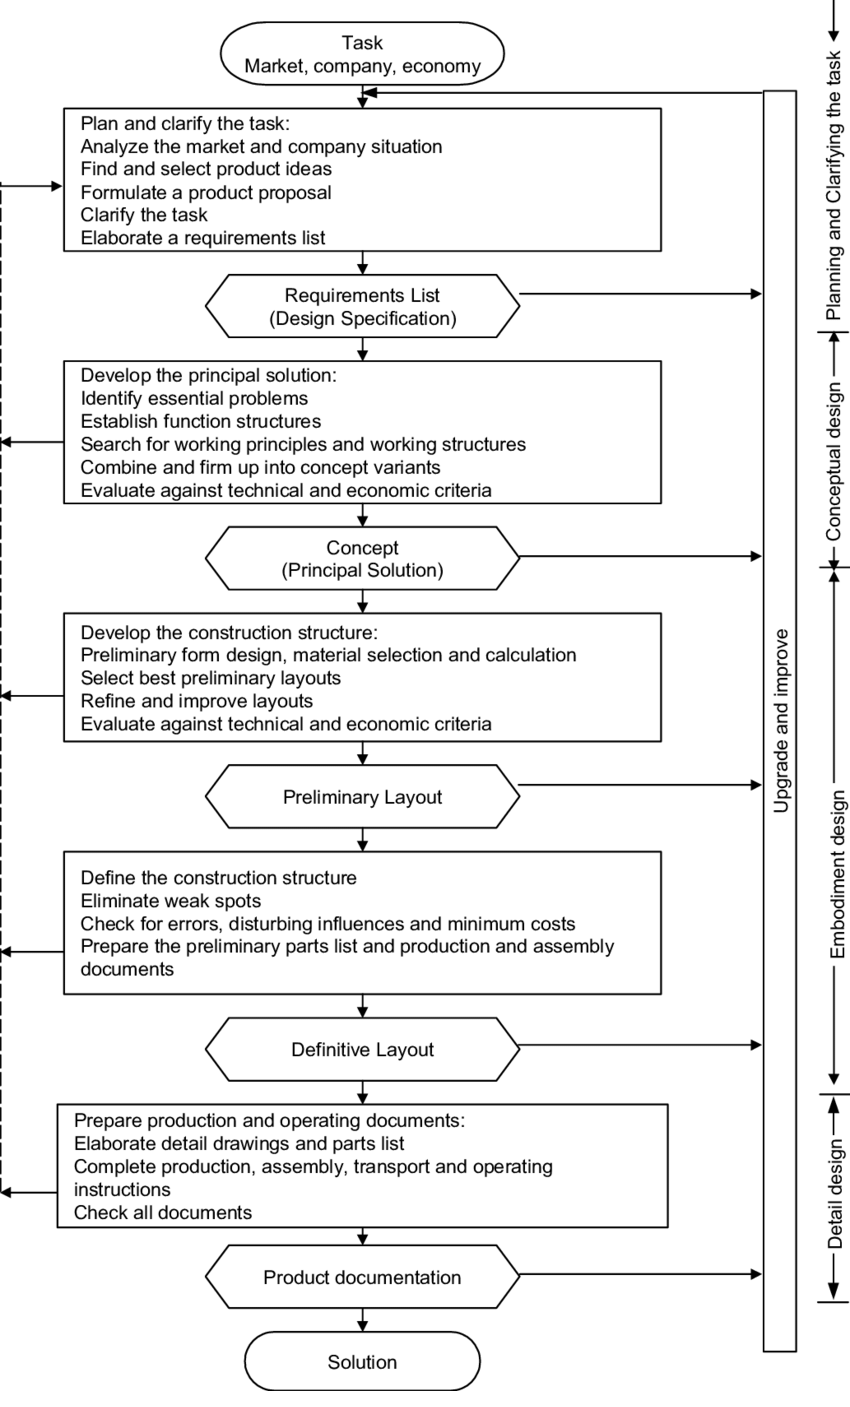
\includegraphics[width=0.75\textwidth]{texs/Part1/chapter1/image/pahlprocess.png}
    \caption{Pahl and Beitz's Design Process \cite{Pahl07l}}
    \label{fig:pahlprocess}
\end{figure}

\section{Fused Deposition Modeling}
\label{sec:fused_deposition_modeling}

Fused deposition modeling (FDM) is a widely used technique in additive manufacturing, particularly in 3D printing. It offers several advantages that contribute to its popularity in various industries. One of the main advantages of FDM is its ability to reproduce complex geometries with high precision and accuracy \cite{Gordeev18}.

This method makes it suitable for creating intricate and customized designs that may not be achievable with traditional manufacturing methods. Additionally, FDM is a cost-effective process as it reduces material waste by only depositing the necessary amount of material layer by layer \cite{Gordeev18}, which not only saves costs but also promotes sustainability in manufacturing.

Common plastics used in FDM include acrylonitrile butadiene styrene (ABS), polylactic acid (PLA), and polyethylene terephthalate (PET) \cite{Teamm17}. These materials have different mechanical properties, advantages, and disadvantages, making them suitable for different applications.

Takahashi et al. \cite{Takahashi17} mentioned that achieving a high-quality printing result necessitates considering various parameters. They classified these factors into four groups: (1) operation parameters, (2) machine parameters, (3) machine parameters, and (4) geometry-specified parameters.

\subsection{Prusa Slicer i3 MK3S+}
\label{subsec:prusa_slicer_mk3s}

The Prusa Slicer i3 MK3S+ is an FDM 3D printer designed for desktop use, ideal for tasks like rapid prototyping and small-scale production. With a build volume of 250 x 210 x 200 mm, it can achieve layer heights ranging from 0.05 mm to 0.35 mm \cite{Prusa}. This printer has a heated bed and is compatible with various materials such as PLA, ABS, PETG, and nylon \cite{Prusa}. The default nozzle size is 0.4 mm, although alternate sizes can be utilized based on specific printing needs.

This 3D printer is accessible to students and faculty at the University of Applied Sciences Brandenburg and will play a pivotal role in the prototype development process. Figure \ref{fig:prusa_slicer_mk3} visually represents the Prusa Slicer i3 MK3S+, located within the University of Applied Sciences Brandenburg Workshop.

\begin{figure}
    \centering
    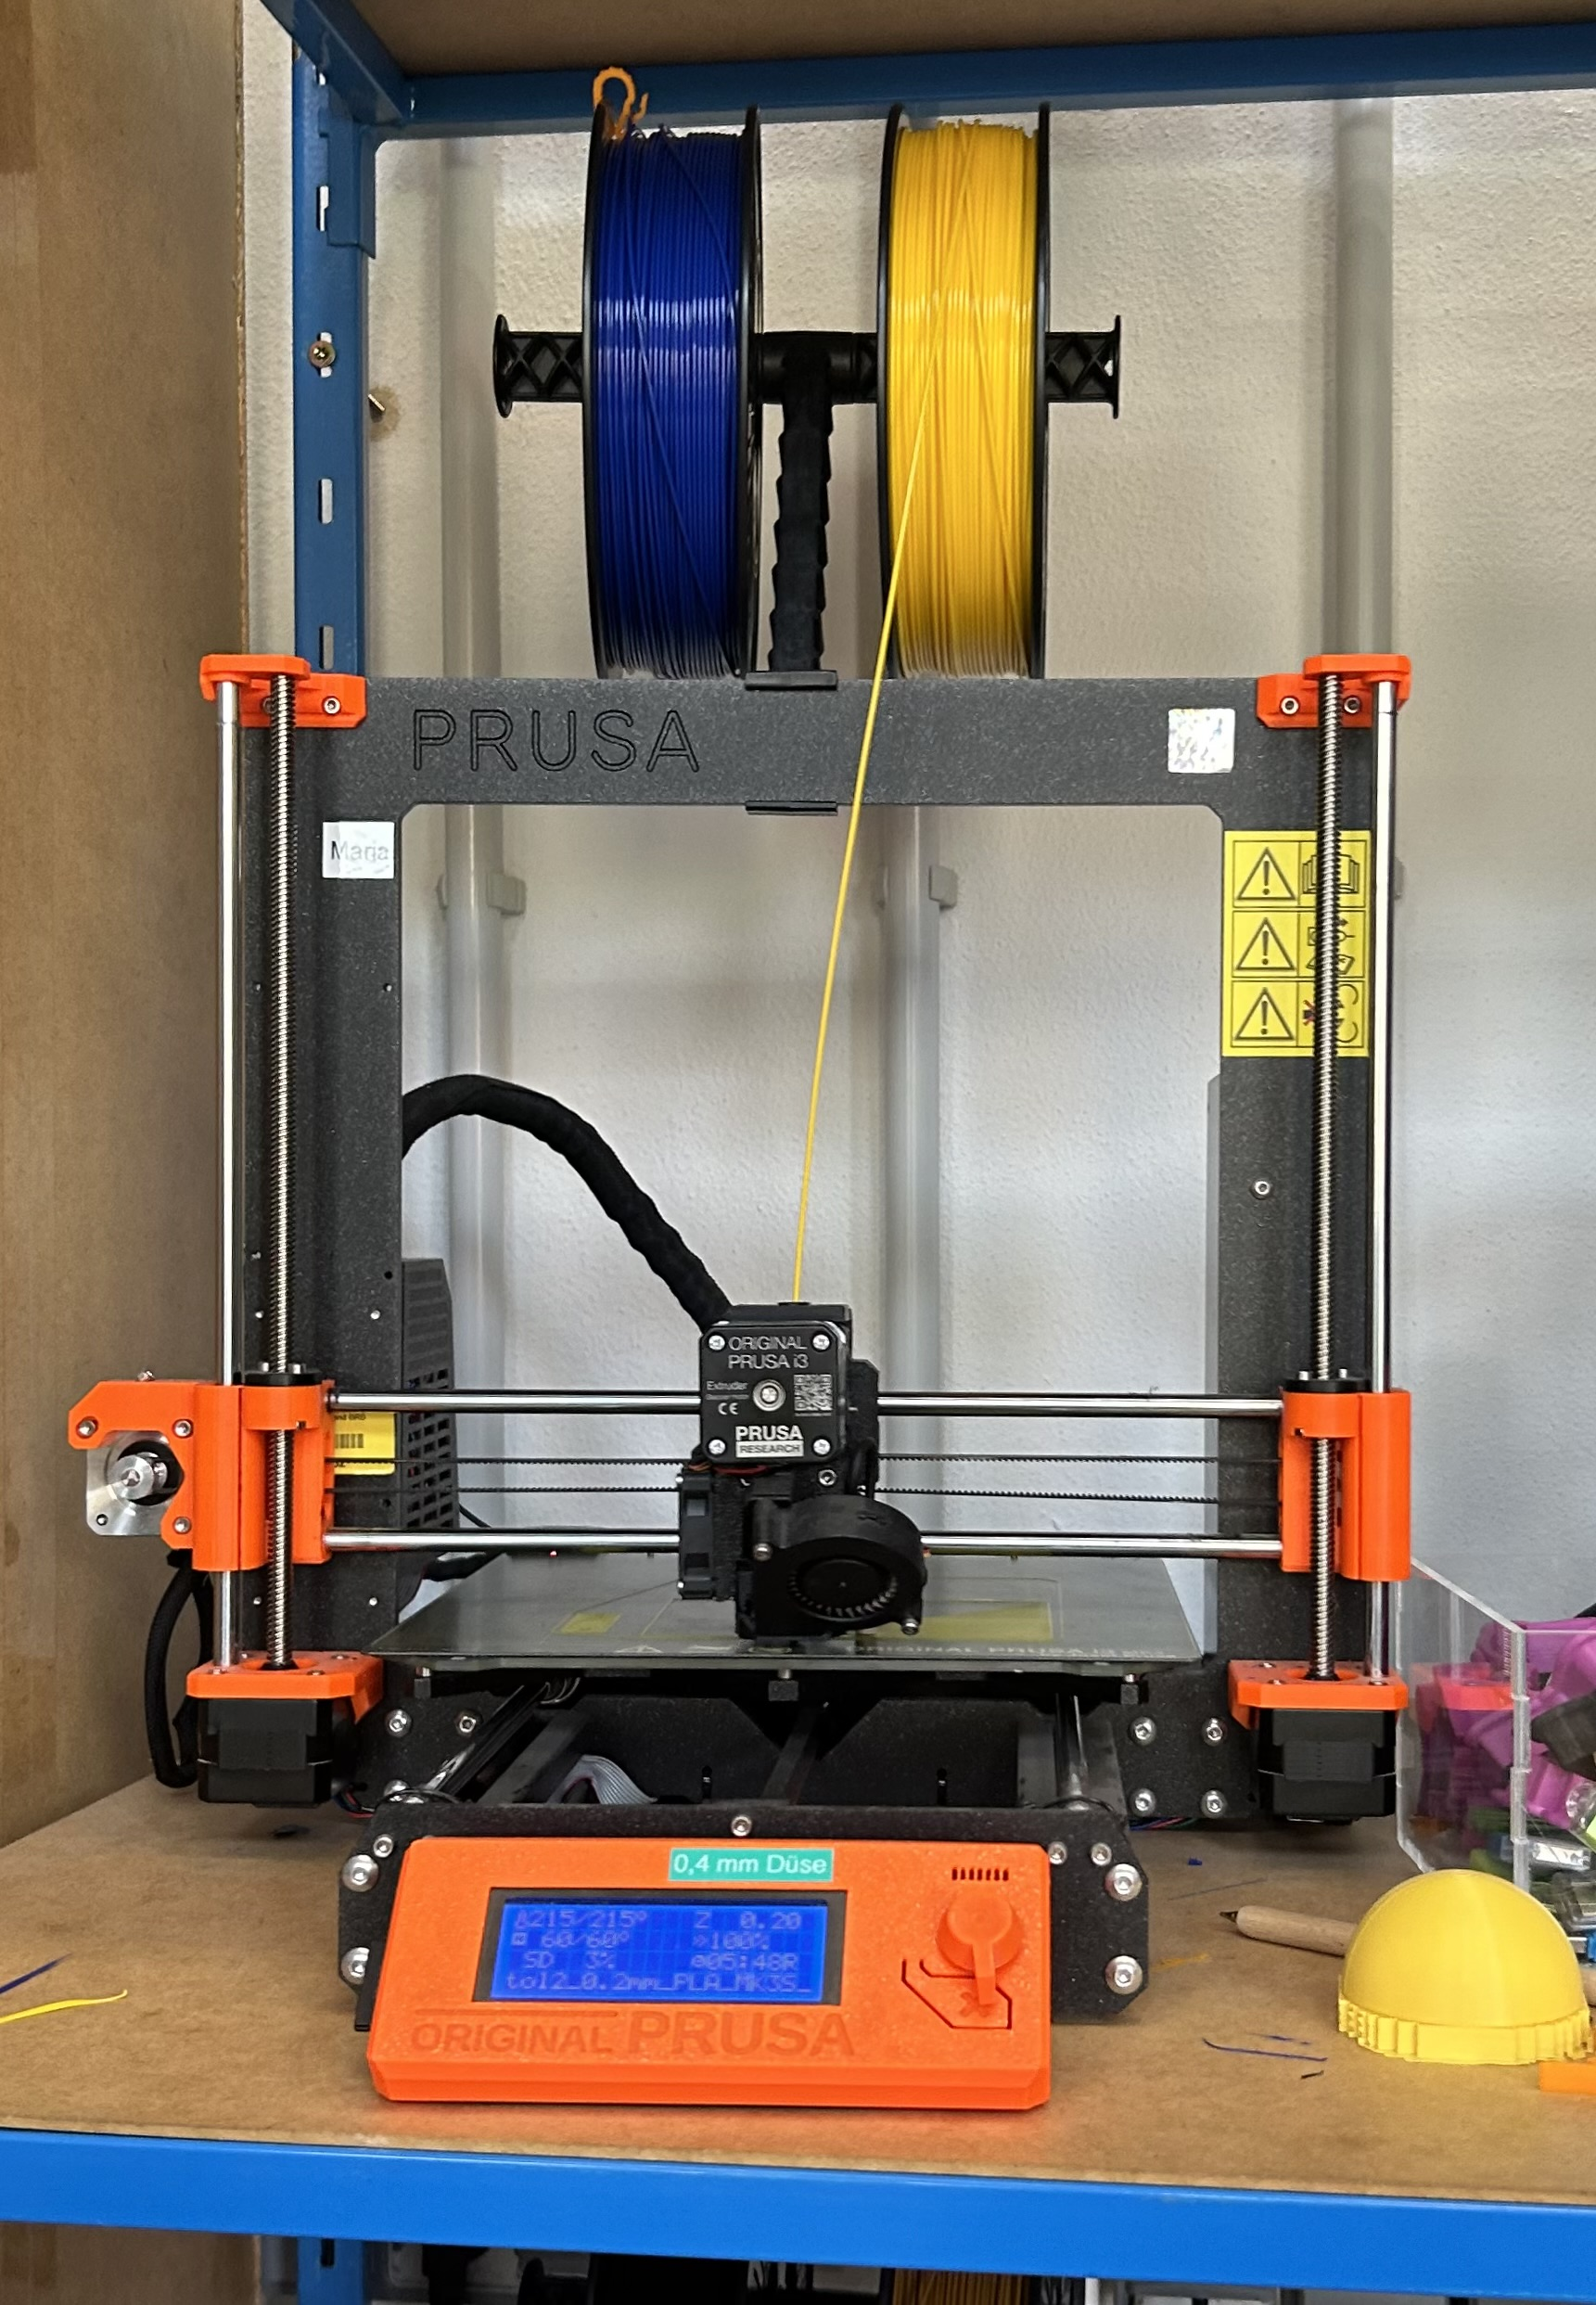
\includegraphics[height=8cm]{texs/Part1/chapter1/image/prusa.jpg}
    \caption{Prusa Slicer i3 MK3S+}
    \label{fig:prusa_slicer_mk3}
\end{figure}

\subsection{PrusaSlicer}
\label{subsec:prusa_slicer}

PrusaSlicer is a free and open-source slicing software that converts 3D models into G-code, a language instructing the 3D printer on printing the object. It is compatible with a wide range of 3D printers and supports a variety of filament materials. PrusaSlicer offers many features that allow users to customize the printing process to suit their needs.

One of the most essential features of PrusaSlicer is the ability to adjust the printing parameters. These parameters include layer height, infill density, and print speed. The layer height refers to the thickness of each layer of the printed object. The infill density refers to the amount of material used to fill the inside of the object. The print speed refers to the speed at which the printer moves while printing the object. These parameters can be adjusted to achieve the desired quality of the final product.

PrusaSlicer offers an essential function of adding support to the 3D prints. Supports are structures that print alongside the object to provide extra stability during printing. They prevent any potential collapse or deformation of the object while printing. Supports can be added manually or automatically depending on the complexity of the printed object.

This software can also generate a preview of the printed object, which lets users visualize the result. Additionally, PrusaSlicer provides an estimate of the amount of filament required for the printing process and the duration of the printing process. Figure \ref{fig:prusa_slicer} shows a screenshot of PrusaSlicer.

\begin{figure}
    \centering
    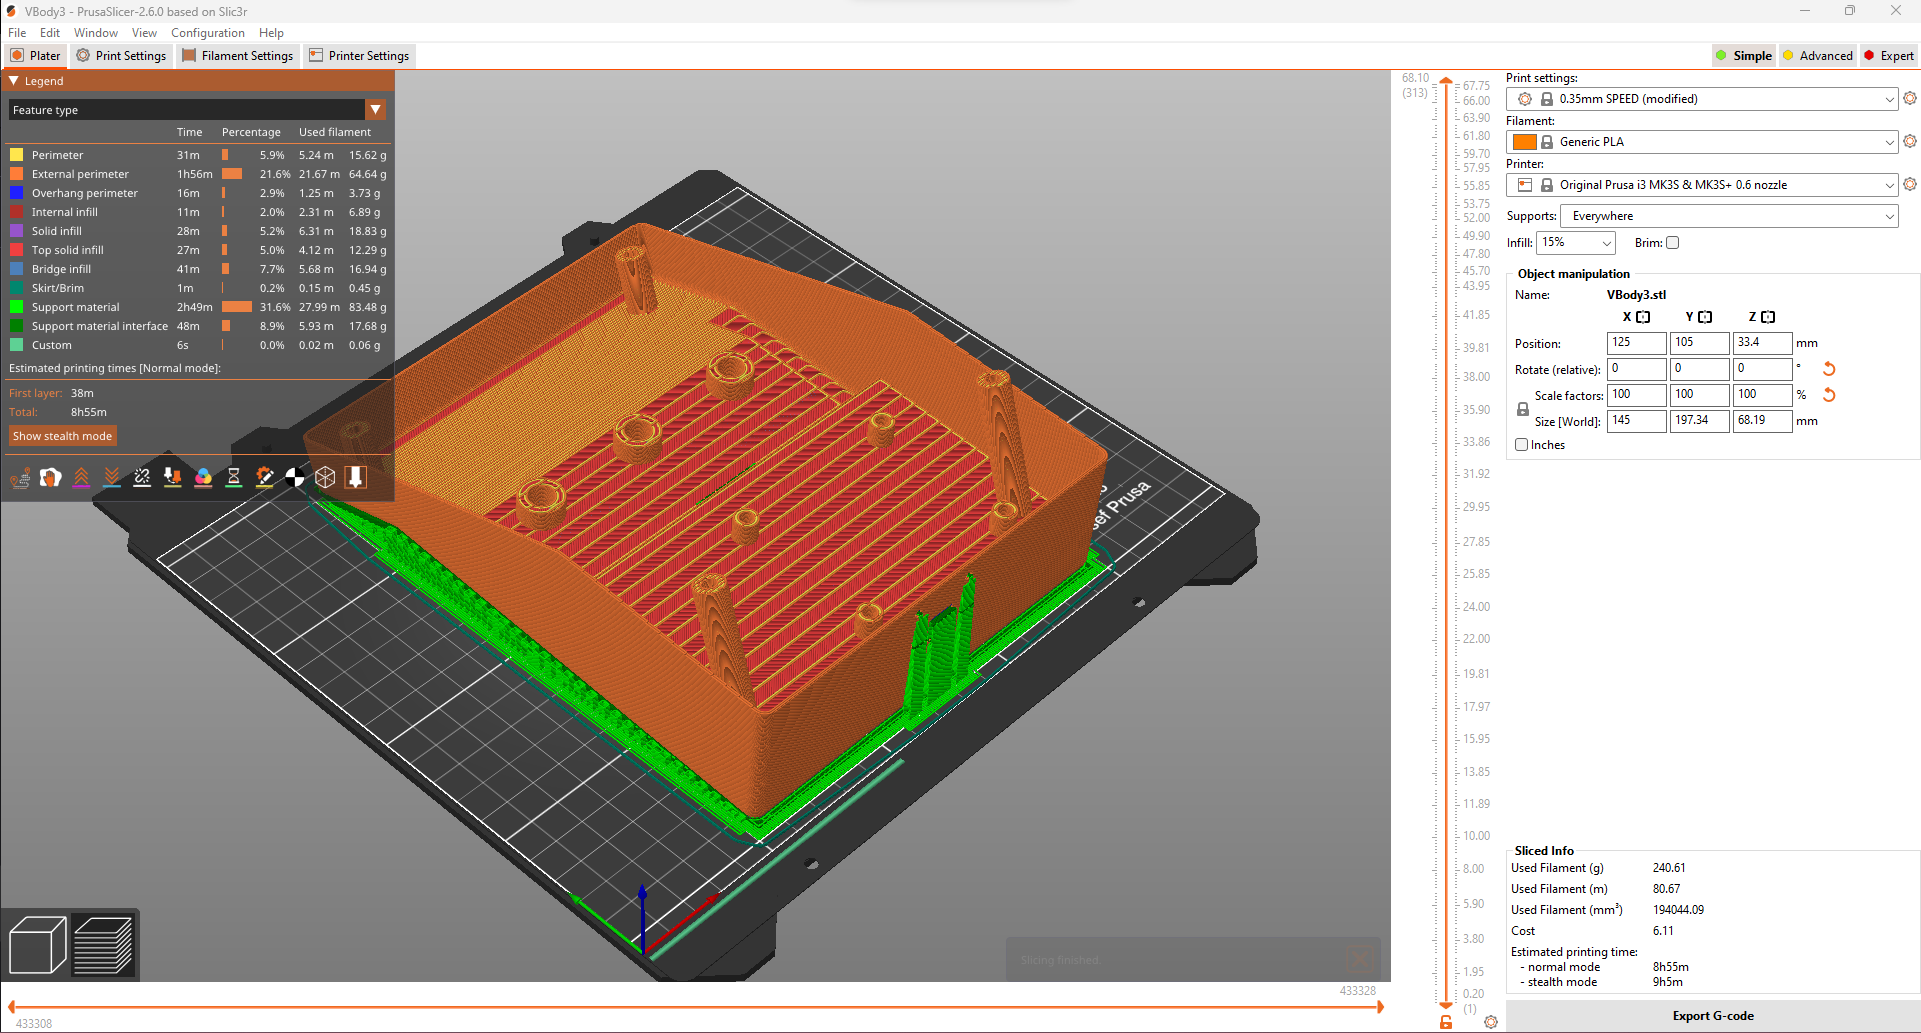
\includegraphics[width=0.8\linewidth]{texs/Part1/chapter1/image/prusaslicer.png}
    \caption{Example View of PrusaSlicer}
    \label{fig:prusa_slicer}
\end{figure}


\subsection{Printing Cost}
\label{subsec:printing_cost}

To perform a cost analysis of the 3D printing process, we will consider the following parameters:

\begin{itemize}
    \item Material Cost ($C_m$)
    \item Energy Cost ($C_e$)
\end{itemize}

Equation \ref{eq:material_cost} shows the formula used to calculate the material cost. This formula involves multiplying the mass of filament used ($m_{fil}$) by the cost of filament per kilogram($C_{fil}$). The cost of the filament is dependent on the type of material used. We will use PLA for this project, which costs 29.99 €/kg \cite{PrusaCost}.

Energy cost refers to the electricity cost of the printing process and is calculated using Equation \ref{eq:energy_cost}. The printing duration ($t_p$) is estimated directly from the PrusaSlicer software, while the power consumption ($P$) of the printer is estimated to be about 0.08 kW \cite{Prusa}. By observing the average price of electricity in Germany for the year 2022 \cite{NordPool}, the electricity price ($C_{el}$) is estimated at 0.235 €/kWh.

Equation \ref{eq:printing_cost} shows the formula for calculating the cost of 3D printing.

\begin{equation}
    \label{eq:material_cost}
    C_{m} = m_{fil}\cdot C_{fil}
\end{equation}

\begin{equation}
    \label{eq:energy_cost}
    C_{e} = t_{p}\cdot C_{el}\cdot P
\end{equation}

\begin{equation}
    \label{eq:printing_cost}
    C_{print} = C_{m} + C_{e}
\end{equation}



\chapter{Planning and Task Clarification}

This chapter delves into the process of planning and clarifying tasks for the prototype, as depicted in Figure \ref{fig:planning} following Pahl and Beitz's model. As mentioned previously in Chapter \ref{sec:methodicproductdevelopment} this step play a critical role in the product development process. They involve precisely defining and understanding the requirements and expectations related to a specific task or project. The aim is to remove any confusion and ensure that everyone involved has a shared understanding of what needs to be achieved.

\begin{figure}[ht!]
    \centering
    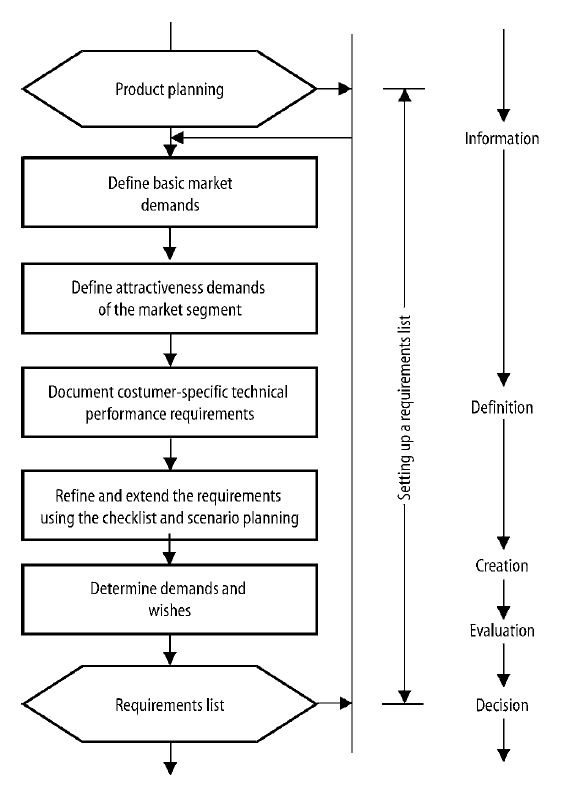
\includegraphics[width=0.6\textwidth]{texs/Part1/chapter2/image/planning.png}
    \caption{Planning and Task Clarification \cite{Pahl07m}}
    \label{fig:planning}
\end{figure}

During this step, the specific goals, limitations, and things that need to be produced for the task are identified \cite{Pahl07a}. By clarifying and specifying tasks, engineers and designers set a strong foundation for the later stages of product development. This allows them to move forward with a clear sense of direction and focus. To achieve this, Pahl and Beitz formulated a series of questions that must be answered to ensure that the task is well-defined and understood \cite{Pahl07a}. These questions are:

\begin{itemize}
    \item What is the objectives of the solution?
    \item What characteristics should the solution have?
    \item What characteristics should the solution avoid?
\end{itemize}

By answering these questions, the requirements for the solution can be identified and spelled out. These requirements will serve as the basis for the subsequent phases of the product development process. The outcome of this step is a list of requirements that outline the needs, expectations, and restrictions tied to the task \cite{Pahl07a}.

\section{Establishing the Prototype's Requirements}
To properly establish the requirements for the prototype, it is suggested to propely define the objectives of the prototype and clearly divide them into demands and wishes \cite{Pahl07n}.

Demands, as described by Pahl and Beitz \cite{Pahl07n}, are the essential and non-negotiable requirements that must be fulfilled for the product to be considered successful. They represent the core functionality and characteristics that the product must possess to meet its intended purpose and provide value to the users. Demands are typically based on objective criteria and are crucial for ensuring the product's basic functionality and compliance.

On the other hand, wishes are defined as the desirable but non-essential requirements or features that stakeholders would like to see in the product. Wishes often involve additional functionalities, aesthetics, or user experience enhancements that would provide added value or differentiate the product in the market. While wishes may not be mandatory, they can contribute to customer satisfaction, competitive advantage, and overall product excellence.

In addition, all of the requirements defined is possible must be quantifiable. This means that the requirements must be measurable and testable. This is important for ensuring that the requirements are met and that the product is able to fulfill its intended purpose.


\section{Identifying the Prototype's Requirements}
In this section, the requirements of the prototype will be established. The checklist (see Figure \ref{fig:checklist}) will be used as a guideline to ensure that all the requirements are properly identified and defined.

\begin{figure}[ht!]
    \centering
    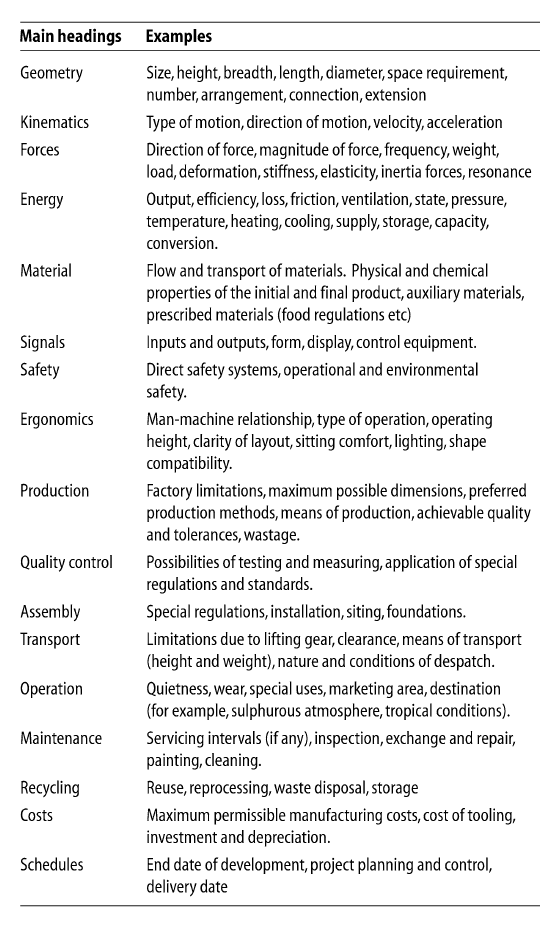
\includegraphics[width=0.6\textwidth]{texs/Part1/chapter2/image/requirements.png}
    \caption{Checklist for Establishing the Prototype's Requirements \cite{Pahl07o}}
    \label{fig:checklist}
\end{figure}

\subsection{Geometry}
When creating a prototype, it's crucial to get its size and shape right so that people can use it effectively. The size determines how big the prototype is and how well it functions. However, we need to be mindful not to make the prototype too large due to manufacturing limitations.

For our prototype, we're utilizing a 3D printing service provided by TH Brandenburg. We're specifically using the Original Prusa i3 MK3S+ 3D printer, which has a maximum printing area of 210 mm by 210 mm by 250 mm \cite{Prusa}. This means we have to work within these size constraints.

To ensure that our prototype fits within these limits, we've decided to slightly reduce its size. We're making it about 10\% smaller than the maximum printing area. This adjustment ensures that our prototype can be comfortably accommodated on the 3D printer at TH Brandenburg. Given these considerations, the largest dimensions we've chosen for the prototype are 190 mm by 190 mm by 220 mm.

\subsection{Energy}
The energy needed for the prototype is really important because it affects how useful and convenient it is. We\'ve made a requirement that the prototype should be able to work on its own for at least 1 hour using the provided power supply. This rule is in place to make sure the prototype can work by itself and give users a smooth experience.

By being able to work for at least 1 hour, the prototype shows that it can keep running for a reasonable amount of time without needing to be charged often or relying on outside power. This enables users to operate the device without concern for an extended period, offering more opportunities to explore its functionality and capabilities. It also provides users with the freedom to engage with the prototype in real-life scenarios, offering valuable insights into its performance and effectiveness.

\subsection{Forces}
The force requirement for the prototype has two main aspects: ensuring it can handle the weight of its components while also adhering to a maximum weight limit.

Firstly, it's crucial to verify that the prototype can effectively support the weight of its components without compromising its overall structure or functionality. This ensures the prototype's durability and ability to withstand the forces exerted by its components. Additionally, it guarantees that the prototype can be manipulated and operated without the risk of damage or malfunction.

Furthermore, there is a specific constraint that the total weight of the prototype must not surpass 2 kg. This encompasses the collective weight of all internal components, including both the predefined components and any additional materials integrated during the design process. Adhering to this weight limit ensures the prototype remains lightweight and manageable, while still meeting the intended performance criteria.

\subsection{Materials}
When crafting the prototype, it's crucial to carefully consider the specific materials and components that will be used. In this project, there are certain components that have already been chosen, and they must be included to meet the requirements. These components include the Raspberry Pi 4B, a 7-inch touch screen, the Raspberry Pi Camera V2, and the Veektomx 10000mAh power bank.

These chosen components act as essential building blocks for the prototype's function and performance. The Raspberry Pi 4B, a versatile single-board computer, supplies computing power and functions as the core control unit for the prototype. The 7-inch touch screen enhances user interaction by providing a responsive and user-friendly interface for input and output.

The Raspberry Pi Camera V2 enables the capture of images and videos, allowing for a range of applications within the prototype. Lastly, the Veektomx 10000mAh power bank provides a dependable power source, ensuring continuous operation of the prototype.

\subsection{Ergonomics}
When it comes to ergonomics, the prototype has specific demands concerning its dimensions, mass, and how users hold it. First and foremost, the prototype needs to be compact and lightweight. This guarantees that it's easy to carry around, making it simple to handle and move. By minimizing the prototype's size and weight, it enhances user comfort and convenience during use.

Furthermore, a vital aspect of the ergonomics requirement is that users should be able to hold the prototype comfortably. This involves thinking about the prototype's shape, grip, and balance to ensure it's easy and secure to hold. The design should fit naturally into the contours of the user's hand, ensuring a stable and ergonomic grip. By optimizing the prototype's shape and considering user ergonomics, it can deliver a smooth and user-friendly experience.

\subsection{Production}
The production requirement for the prototype focuses on the manufacturing process and the materials used. The prototype must be designed to be manufactured using 3D printing technology. This ensures that the prototype can be produced using the available resources and capabilities. In addition, the prototype must be designed to be manufactured using PLA filament. This material is readily available and offers a good balance of strength and flexibility, making it suitable for the prototype's requirements.

\subsection{Operation}
The operation requirement for the prototype encompasses two key aspects: the ability to be used freehand and the capability to integrate with a tripod for improved stability.

Firstly, the prototype must be designed to facilitate freehand operation. This means that users should be able to interact with and operate the prototype comfortably and conveniently without the need for additional support or mounting. The design should consider ergonomic factors such as grip, button placement, and user-friendly controls, ensuring that users can manipulate the prototype easily and intuitively.

Secondly, the prototype should be capable of integrating with a tripod for enhanced stability when necessary. This feature allows users to attach the prototype securely to a tripod, providing a stable and stationary setup. By integrating tripod compatibility, the prototype can cater to scenarios where steady and controlled operation or positioning is required, such as capturing images or conducting experiments that demand minimal movement.

\subsection{Assembly}
The assembly requirement for the prototype emphasizes the importance of considering the ease of assembly and disassembly of its components. This design consideration enables users to access the inner components easily, facilitating maintenance and repair tasks.

By designing the prototype with ease of assembly in mind, it becomes simpler for users to put the components together without requiring complex tools or specialized knowledge. This promotes user-friendliness and reduces the time and effort required for initial assembly or subsequent modifications. Similarly, easy disassembly allows users to access the internal components when needed, simplifying troubleshooting, repairs, or component replacements.

Additionally, if feasible, the parts of the prototype should be designed with swappable properties. This means that individual components or modules can be easily removed and replaced, without the need to disassemble the entire prototype. Swappable parts enhance modularity, flexibility, and cost-effectiveness, as users can upgrade or replace specific components as needed, rather than replacing the entire prototype.

\subsection{Costs}
The cost requirement for the prototype focuses on the total cost of production. The prototype must be designed to be manufactured within a budget of 100 euros excluding the cost of the predefined components. This budget encompasses the cost of all materials and components used in the production process. By adhering to this cost limitation, the prototype can be produced within the available resources and capabilities.

\subsection{Schedules}
The schedule requirement for the prototype focuses on the time required for production. The prototype must be designed to be manufactured within a time frame of 2 weeks. This time frame encompasses the entire production process, from design to assembly. By adhering to this schedule, the prototype can be produced within the available resources and capabilities.

\subsection{Durability}
The durability requirement for the prototype includes considerations for resistance to dust and water, if feasible. While it may not always be possible to achieve complete resistance, efforts should be made to enhance the prototype's durability in these aspects.

Regarding dust resistance, the prototype should be designed to minimize the ingress of dust particles into its internal components and sensitive areas. This involves employing appropriate seals, filters, or protective enclosures to prevent dust from adversely affecting the prototype's performance or functionality. By reducing the risk of dust accumulation, the prototype can maintain its optimal operation and extend its lifespan.

In terms of water resistance, if feasible and relevant to the intended use, the prototype should exhibit a level of protection against water ingress. This can involve incorporating waterproof or water-resistant materials, seals, or coatings to shield the internal components from moisture. Ensuring water resistance enhances the prototype's durability and enables usage in environments where exposure to water or humidity is likely.

\section{Requirement List}
Table 1 and Table 2 on the following pages show the requirements list which included the requirements described in this chapter.

\chapter{Conceptual Design}
Following the clarification of the task is the conceptual design, where in this section of the product development process, designers engage in creative exploration and evaluation of various design ideas and concepts.

According to Pahl and Beitz, conceptual design is the stage of the design process where important issues are pinpointed through abstraction  \cite{Pahl07d}. The process involves establishing function structures, searching for suitable working principles, and ultimately combining these elements to create a working structure.

Figure \ref{fig:steps-conceptual-design} shows the steps involved in this phase.

\begin{figure}[ht!]
    \centering
    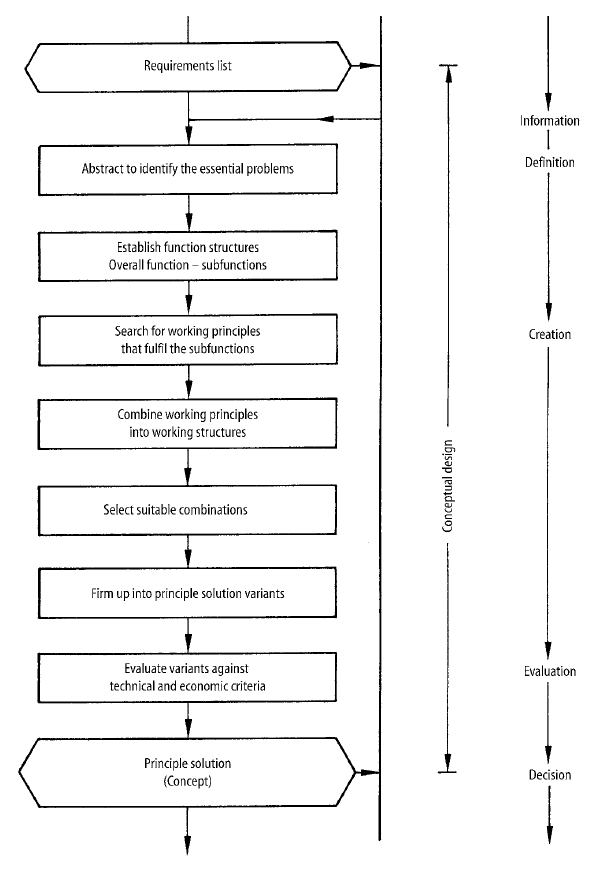
\includegraphics[width=0.7\linewidth]{texs/Part1/chapter3/image/conceptual.png}
    \caption{Steps in Conceptual Design \cite{Pahl07p}}
    \label{fig:steps-conceptual-design}
\end{figure}


\section{Abstraction}
Due to new technologies, procedures, materials, and scientific discoveries, traditional solution principles or designs may not be able to provide optimal answers, and to overcome fixation on conventional ideas, designers utilize abstraction, focusing on the general and essential aspects rather than particular details \cite{Pahl07b}.

To help in identification of the essential problems, following abstraction techniques are used \cite{Pahl07c}:

\begin{itemize}
    \item \textbf{Step 1:} Eliminate personal preferences.
    \item \textbf{Step 2:} Omit requirements that have no direct bearing on the function and the essential constraints.
    \item \textbf{Step 3:} Transform quantitative into qualitative data and reduce them to essential statements.
    \item \textbf{Step 4:} Generalise the previous step's results.
    \item \textbf{Step 5:} Formulate the problem in solution-neutral terms.
\end{itemize}

Figure \ref{fig:result-abstraction-process} shows the result of the abstraction process.

\begin{figure}[ht!]
    \centering
    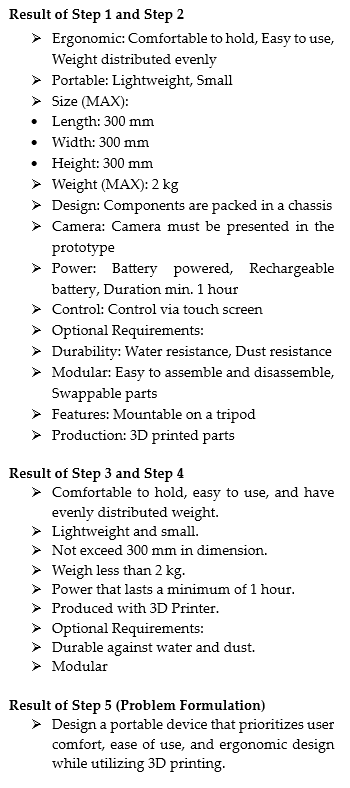
\includegraphics[width=0.4\linewidth]{texs/Part1/chapter3/image/abstractionresult.png}
    \caption{Result of Abstraction Process}
    \label{fig:result-abstraction-process}
\end{figure}


\section{Function Structures}
Pahl and Beitz \cite{Pahl07e} define function structures as a graphical representation of the functions of a system and their interrelationships. It is a hierarchical representation of the functions of a system, starting with the overall function and breaking it down into sub-functions. The function structure is a helpful tool for identifying a system's essential functions and the relationships between the functions.

Figure \ref{fig:subfunction-break} shows the representation of the function structure and the process of breaking down the overall function into sub-functions.

\begin{figure}[ht!]
    \centering
    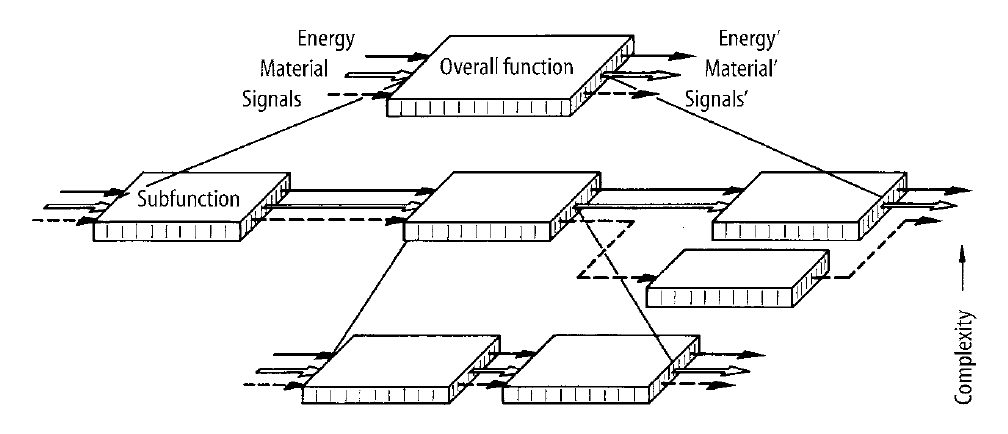
\includegraphics[width=0.8\linewidth]{texs/Part1/chapter3/image/subfunctionbreak.png}
    \caption{Breaking down the overall function into sub-functions \cite{Pahl07q}}
    \label{fig:subfunction-break}
\end{figure}


\subsection{Overall Function}
Based on the result of abstraction, the system's overall function can be represented and visualized using a function structure diagram, as shown in Figure \ref{fig:overall-function}.

In this overall function, the prototype's components are defined as an input, while the prototype itself is defined as the output. The overall function is decomposed into sub-functions in the next section.

\begin{figure}[ht!]
    \centering
    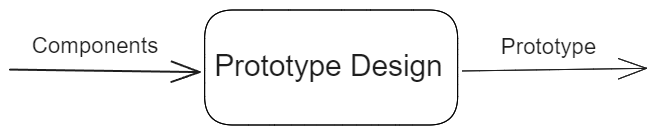
\includegraphics[width=0.5\linewidth]{texs/Part1/chapter3/image/overallfunction.png}
    \caption{Overall Function of the System}
    \label{fig:overall-function}
\end{figure}


\subsection{Sub-Functions}
\begin{figure}[ht!]
    \centering
    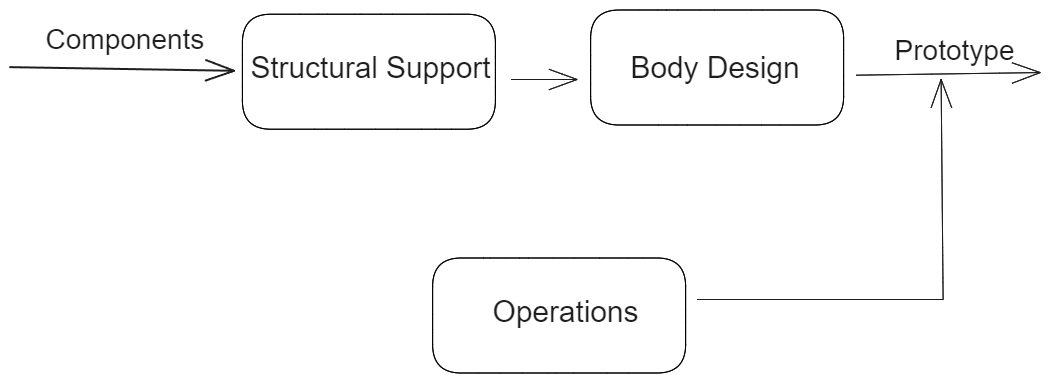
\includegraphics[width=0.8\linewidth]{texs/Part1/chapter3/image/subfunction1.png}
    \caption{Sub-Functions of the System}
    \label{fig:sub-functions}
\end{figure}

\begin{figure}[ht!]
    \centering
    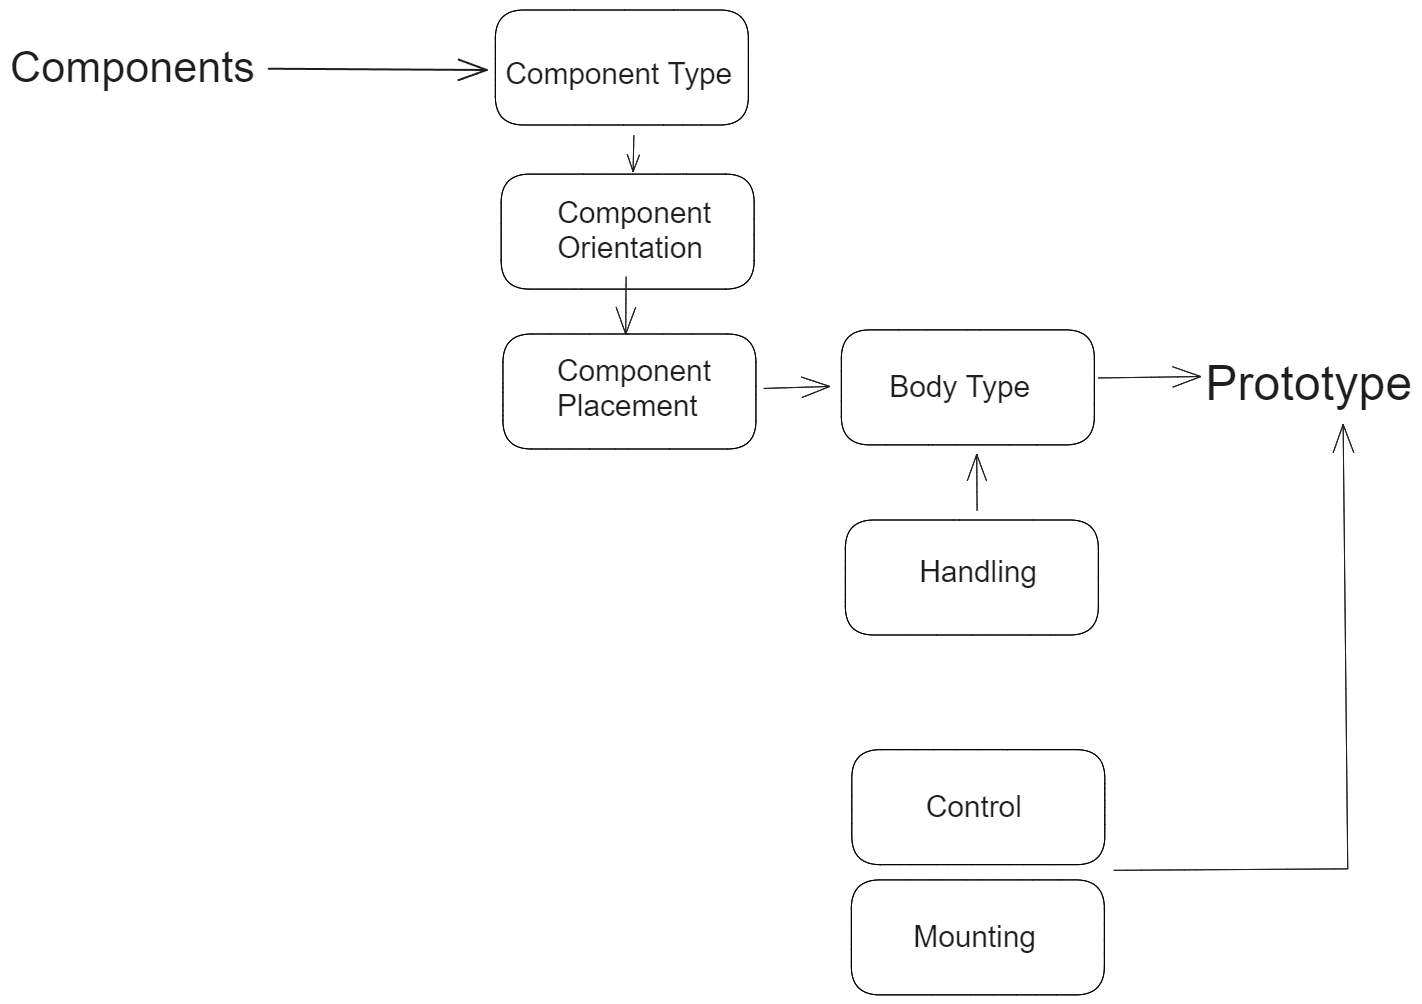
\includegraphics[width=\linewidth]{texs/Part1/chapter3/image/subfunction2.png}
    \caption{Sub-Functions of the System (Final)}
    \label{fig:sub-functions-final}
\end{figure}

Decomposing the overall function into sub-functions is crucial in the conceptual design process, and as described by Pahl and Beitz \cite{Pahl07r}, the purpose of this decomposition is to reduce the complexity of the overall system and facilitate the identification of suitable solution principles that can fulfill the required functions.

Figure \ref{fig:sub-functions} illustrates the sub-functions of the prototype. Deriving from the overall function, labeled as \textit{Prototype Design}, it breaks down into three subfunctions, specifically \textit{Structural Support}, \textit{Body Design}, and \textit{Operation}. The function is then further decomposed into more detailed sub-functions in Figure \ref{fig:sub-functions-final}.

The term \textit{Structural Support} refers to the measures taken to ensure the structural integrity of the prototype. This sub-function encompasses activities such as securing and stabilizing the internal components within the prototype. To simplify the function, it decomposed into three sub-functions:  \textit{Component Placement}, which specifies the positioning of internal components; \textit{Component Orientation}, which details the alignment of internal components; and \textit{Component Type}, which is the type of component itself.

\textit{Body Design} describe the sub-functions involving the prototype's physical structure. To further simplify the task, this sub-function is decomposed into \textit{Body Type}, which defines the outline of the structure, and \textit{Handling}, which describes the handling of the prototype.

\textit{Operation} deals with how the prototype works. It describes the device's usage and the components involved during operation. This function is then divided into \textit{Control Mechanism}, which describes the component involved during operation, and \textit{Integration with External Mounting}, which refers to the integration of the prototype with the tripod stand.

\section{Developing Working Principles}

In developing working structures, one crucial step is to search for working principles. As defined by Pahl and Beitz, working principles refer to the physical effects and characteristics that fulfill specific functions of the designed structure \cite{Pahl07f}. These principles are combined to create the working structure, encompassing physical processes and the form design features. Several potential working structures can be generated by varying the physical effects and form design features, known as the solution field.

In developing working principles, there are multiple available methods in idea generation. These methods are categorized into three groups:

\begin{itemize}
    \item Conventional methods
    \item Intuitive methods
    \item Discursive methods
\end{itemize}

Pahl and Beitz \cite{Pahl07g} describe the \textit{Conventional Methods} as a systematic and data-driven approach. Designers gather information from various sources, such as literature, trade publications, and competitor catalogs, to stay informed about advancements and best practices. They analyze natural systems and existing technical systems to draw inspiration and identify opportunities for improvement. Analogies substitute analogous problems or systems, leading to fresh perspectives. Additionally, empirical studies, such as measurements and model tests, provide tangible data for validating designs and predicting real-world performance.

On the other hand, the \textit{Intuitive Methods}, as described by them \cite{Pahl07h}, tap into creativity and associative thinking. \textit{Brainstorming} fosters a collaborative environment where diverse perspectives generate a wide range of ideas without judgment. \textit{Method 635} adds structure to Brainstorming, allowing for systematic idea development within a group. The \textit{Gallery Method} combines individual work with group discussions, using sketches or drawings to explore solution proposals visually.

Additionally, Pahl and Beitz \cite{Pahl07i} introduce \textit{Discursive methods}, which combines systematic, step-by-step procedures with elements of intuition and creativity. They involve deliberate analysis of physical processes, leading to multiple solution variants derived from the relationships between variables. This approach fosters a deeper understanding of the problem space.

\subsection{Searching for Working Principles}
We utilize multiple techniques, including \textit{Brainstorming} and \textit{Analysis of Existing Technical Systems}, to establish working principles for this project. Brainstorming helps to generate ideas and concepts, while Analysis of Existing Technical Systems enables us to scrutinize and assess the ideas and concepts generated.

Table \ref{tab:classification-scheme-working-principles} shows the result of idea generation. For more detailed sketches of the working principles, please refer to Appendix \ref{appendix:sketches-of-working-principles}.

\begin{table}[H]
    \centering
    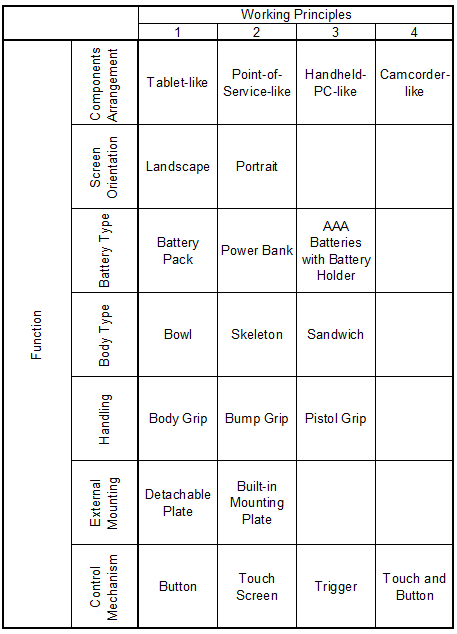
\includegraphics[width=0.6\linewidth]{texs/Part1/chapter3/image/stotal.png}
    \caption{Classification Scheme for Working Principles}
    \label{tab:classification-scheme-working-principles}
\end{table}


\section{Combination of Working Structures}
In this step, we will combine the working principles assigned to the sub-functions to create potential working structures. To achieve this, the identified working principles must be linked following the functional structure to fulfill the overall function.

The method we will employ for systematic combination is Zwicky's morphological box \cite{Kushahrin22}. In this approach, the potential principles are represented in a table for better clarity and connected to form functional structures using connecting lines.

Figure \ref{fig:morphological-chart-with-solution-variants} shows the morphological chart with the generated solution variants. The solution variants are labeled S1 to S9, with each color representing a different solution variant.

\begin{figure}[ht!]
    \centering
    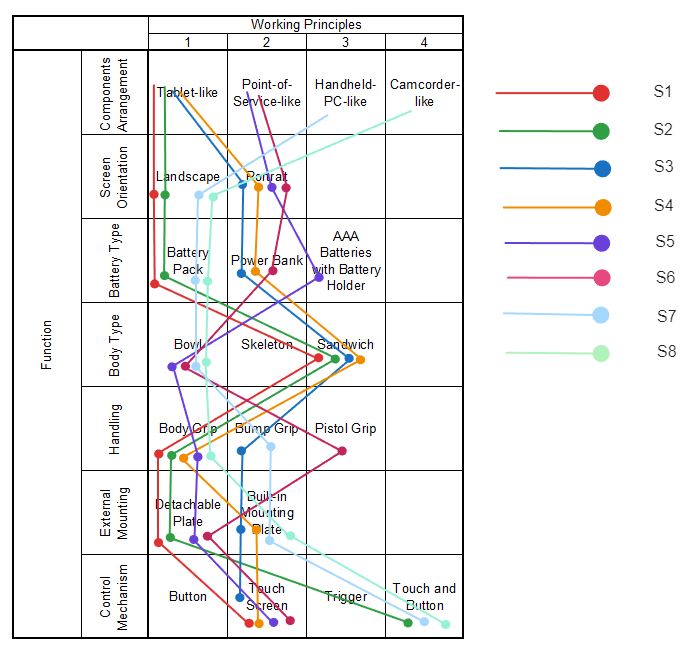
\includegraphics[width=\linewidth]{texs/Part1/chapter3/image/combinedchart.png}
    \caption{Morphological Chart with Solution Variants}
    \label{fig:morphological-chart-with-solution-variants}
\end{figure}

\section{Firming Up into Principle Solution Variants}
In this section, we showcase hand-drawn sketches of identified functional structures that have been transformed into practical solution alternatives. Each sketch is accompanied by a brief description of its operations, highlighting its potential strengths and weaknesses.

\subsection{Solution Variant 1}
In Solution Variant 1, we encounter a tablet-like design that closely resembles a typical tablet device. The key components, including the Raspberry Pi, Battery, Camera, and Screen, are arranged in a manner reminiscent of a tablet. The screen orientation is in landscape mode, offering a broader display view for enhanced visual clarity. This orientation is particularly beneficial when the device is used for tasks that require a wider viewing area.

The design is thoughtfully optimized for handheld use, featuring a body grip that ensures comfortable handling. The internal battery integration contributes to a seamless and integrated appearance. A sandwich-type body provides robust protection for the internal components, comprising a top cover, main body, and bottom cover.

For mounting purposes, Solution Variant 1 utilizes a detachable plate tripod system, offering the convenience of easy attachment and removal from a tripod stand. The primary control mechanism for this variant is a touch screen, allowing for intuitive and user-friendly interactions with the device's functionalities.

\begin{figure}[H]
    \centering
    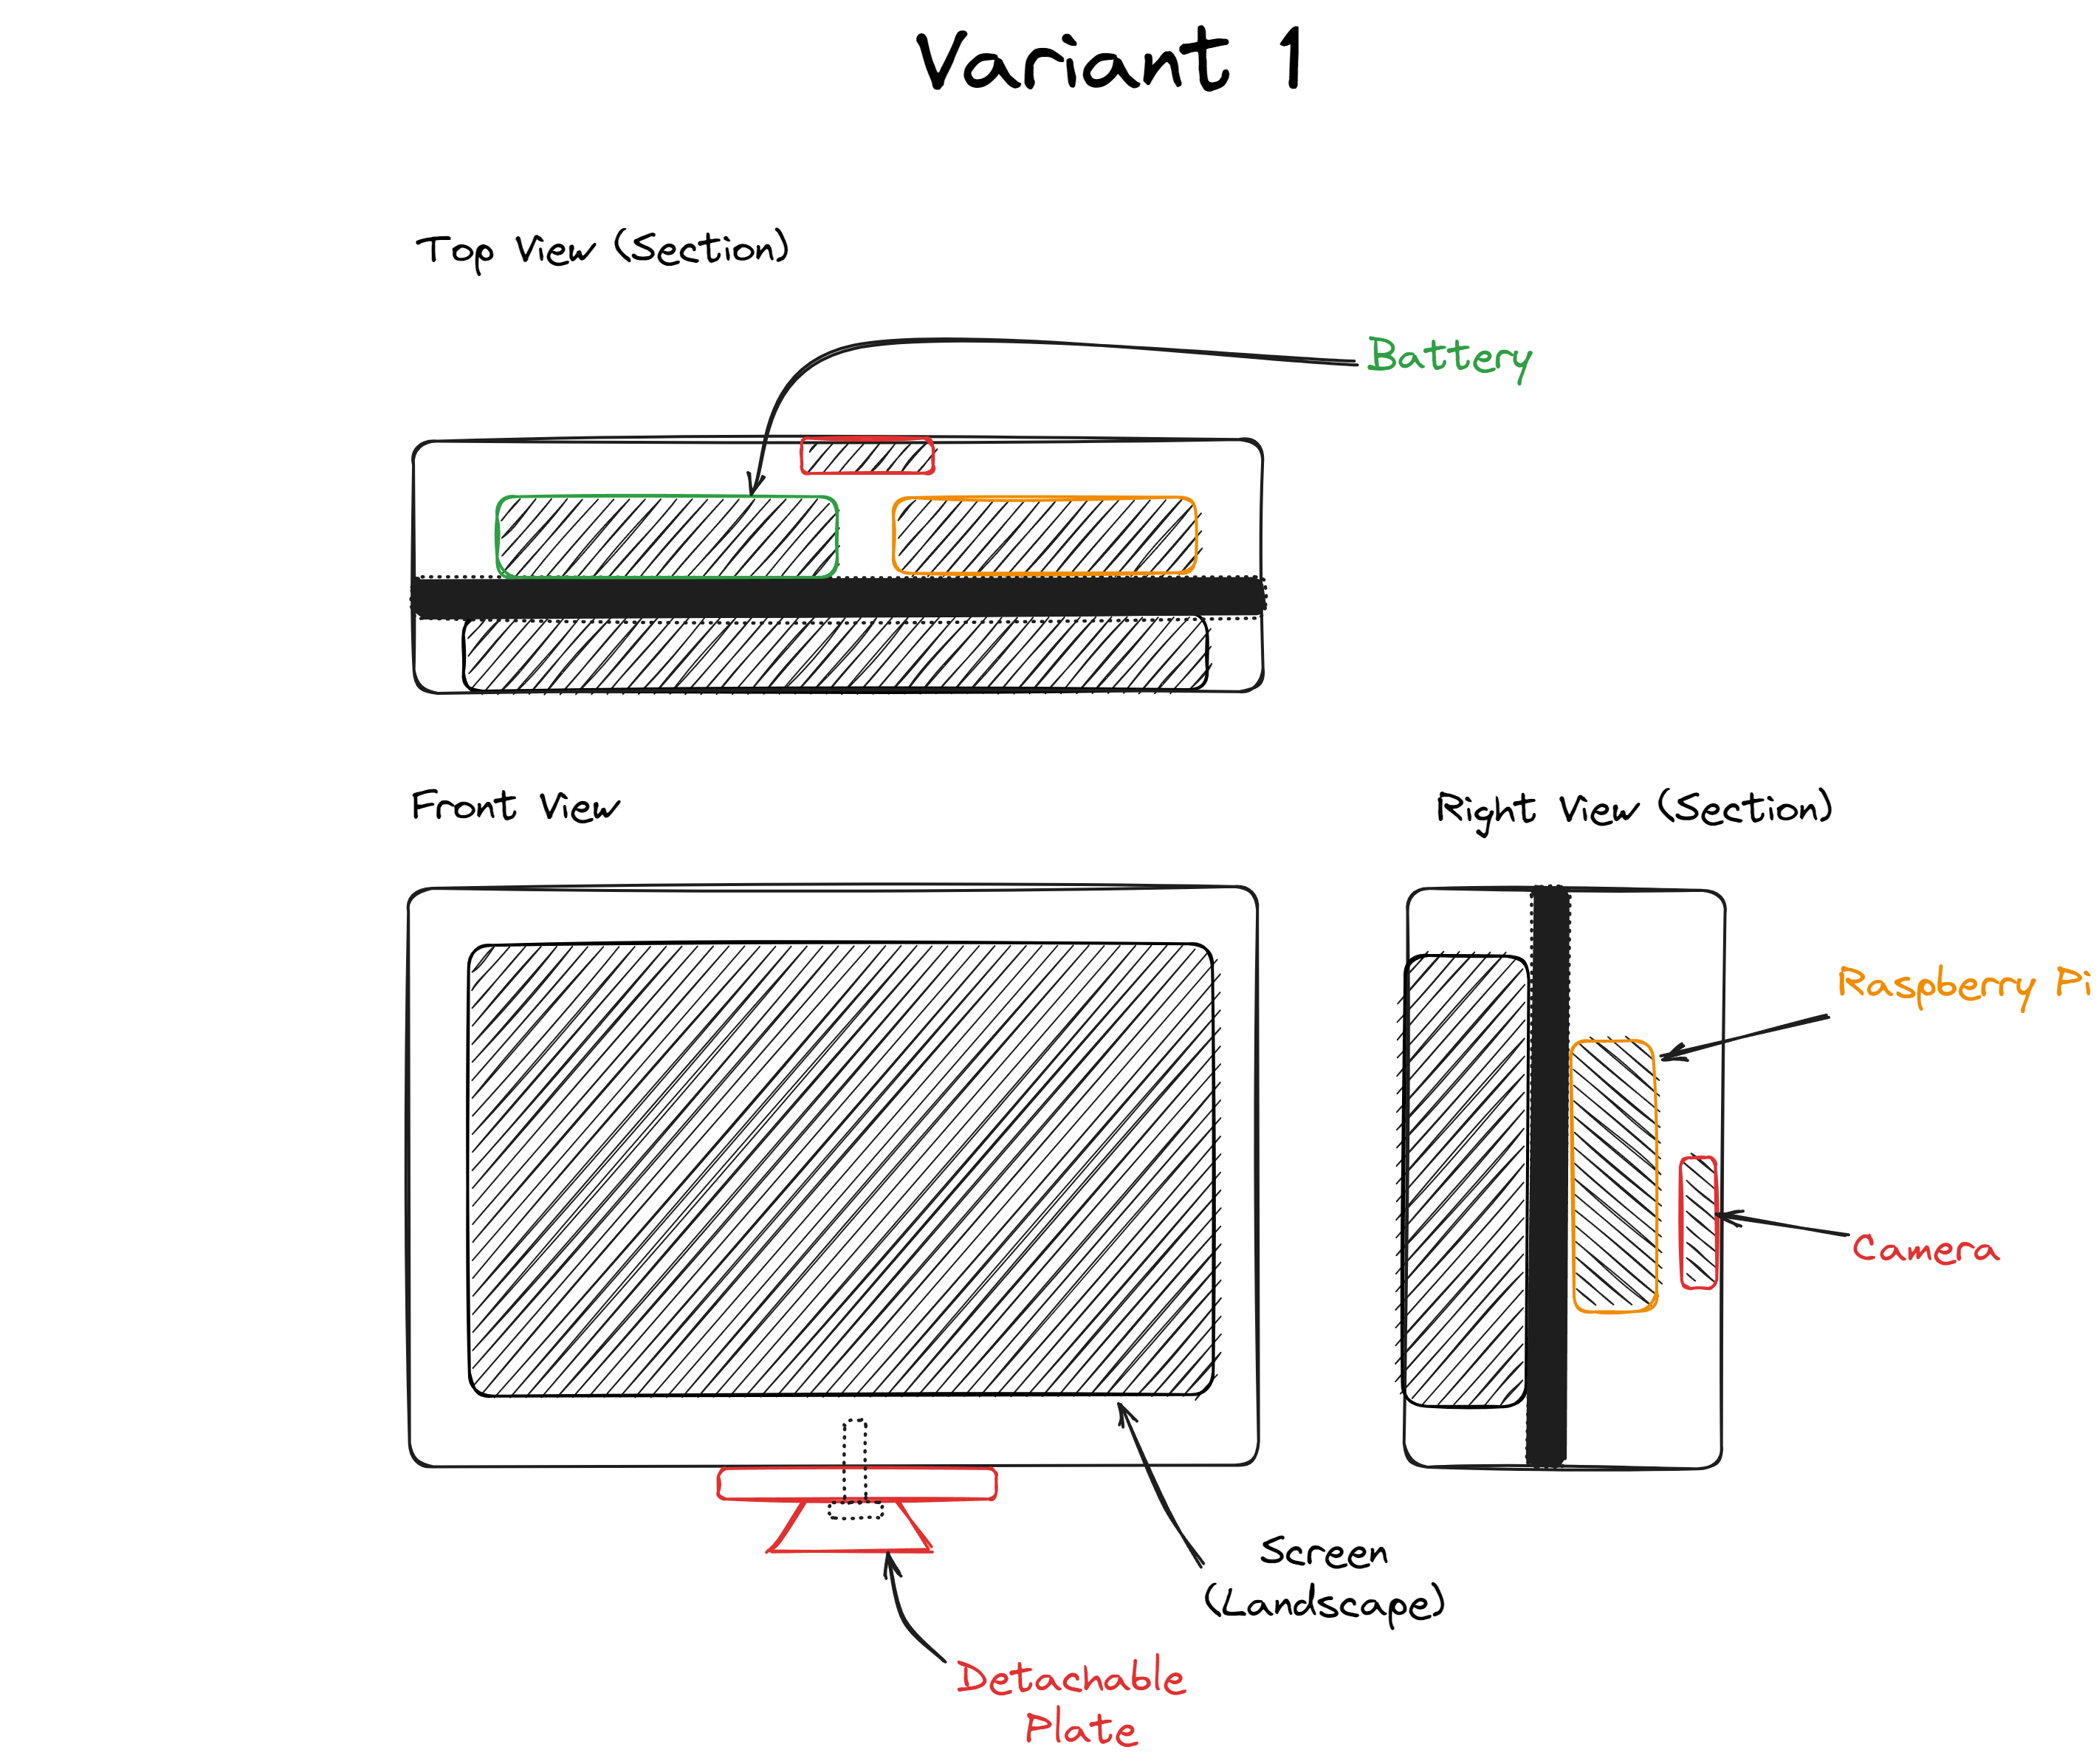
\includegraphics[width=0.75\linewidth]{texs/Part1/chapter3/image/v1.png}
    \caption{Sketch of Solution Variant 1}
    \label{fig:sketch-solution-variant-1}
\end{figure}


\subsection{Solution Variant 2}
Like its predecessor, Solution Variant 2 maintains a tablet-like design, with components arranged like a tablet device. It, too, adheres to a landscape screen orientation for an expansive display view. The device is designed to be comfortably held with a body grip.

One significant difference lies in the battery arrangement. Instead of being integrated, Solution Variant 2 opts for a battery pack, potentially offering the advantages of easier replacement and extended usage periods. Like Solution Variant 1, it employs a sandwich-type body structure for sturdy protection of internal components.

The detachable plate tripod system is retained in terms of mounting, ensuring compatibility with tripod stands. What sets Solution Variant 2 apart is the inclusion of physical buttons alongside the touch screen as the primary control mechanism. This addition enhances versatility and usability in various scenarios, as users can choose between touch-based and tactile input.

\begin{figure}[H]
    \centering
    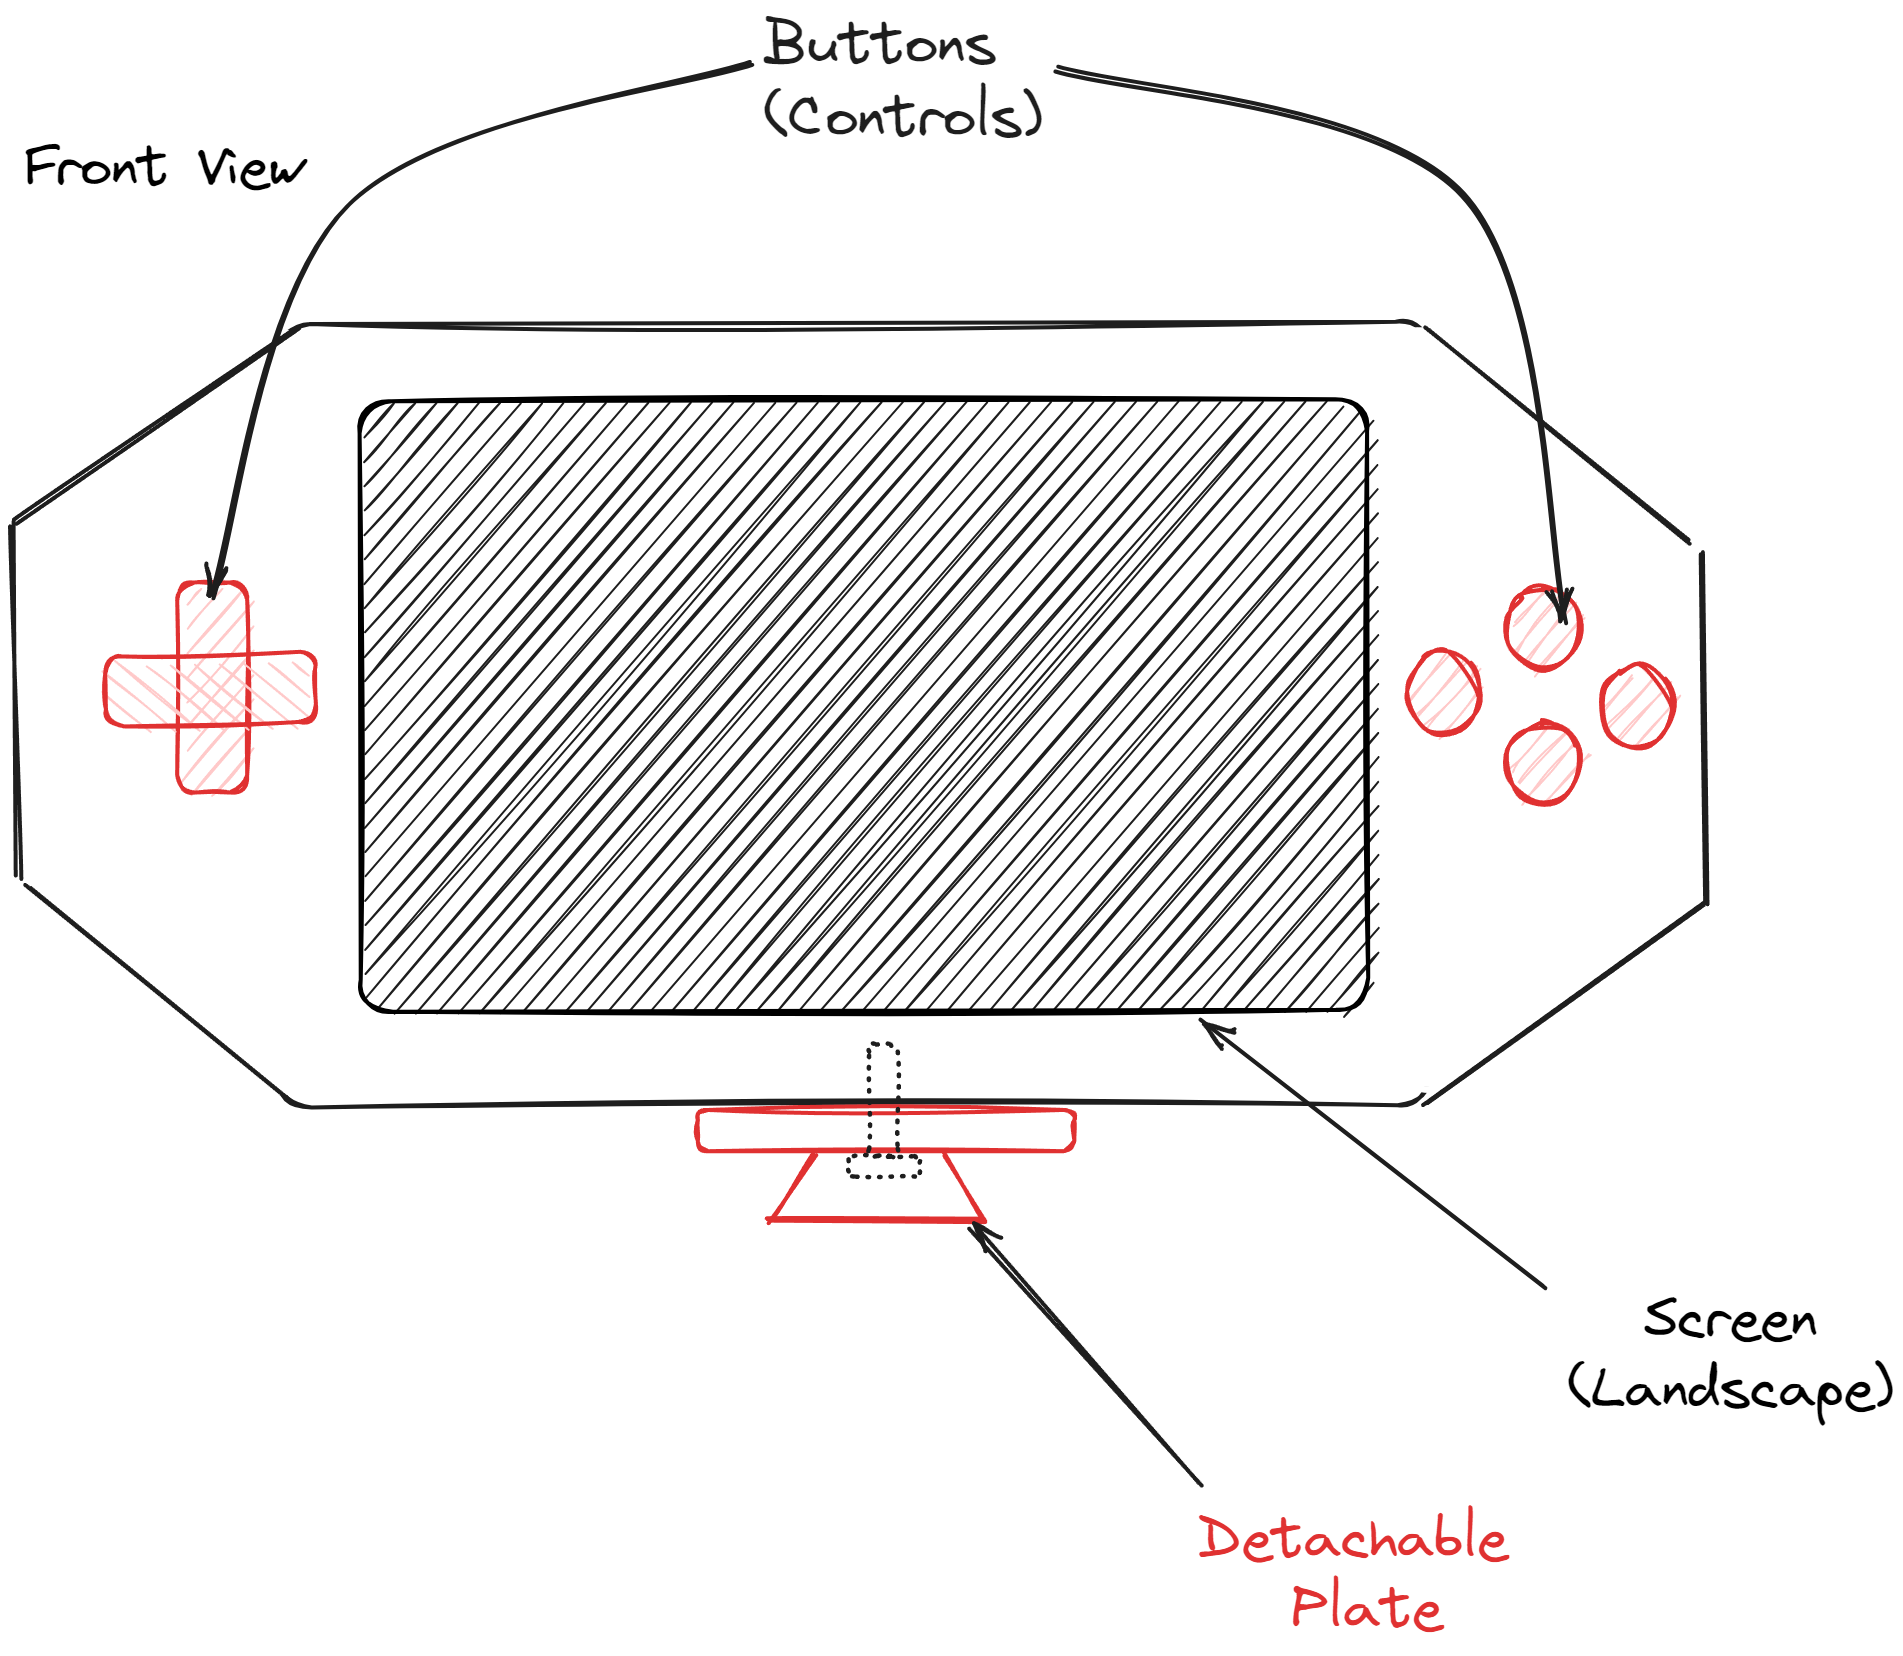
\includegraphics[width=0.55\linewidth]{texs/Part1/chapter3/image/v2.png}
    \caption{Sketch of Solution Variant 2}
    \label{fig:sketch-solution-variant-2}
\end{figure}

\subsection{Solution Variant 3}
While Solution Variant 3 maintains the tablet-like component placement found in the previous variants, it introduces a significant change by adopting a portrait screen orientation. This shift opens up new possibilities for the device's usage, particularly in scenarios where vertical screen space is more advantageous than horizontal layout.

The design includes a bump grip for secure and comfortable handling in a vertical position. Notably, the battery is positioned externally in this variant, offering the potential advantage of easier access and replacement. The body structure remains a sandwich-type, providing robust protection for the internal components.

A fixed mounting plate is employed, ensuring a stable attachment to a tripod stand. Similar to the earlier variants, Solution Variant 3 relies on a touch screen as the primary control mechanism, facilitating intuitive and user-friendly interactions.

One notable advantage of the portrait screen orientation is the improved stability of the device, as the center of gravity is aligned with the device's center. This alignment enhances balance and control when using the device in various orientations, thus enhancing overall usability and versatility.

\begin{figure}[H]
    \centering
    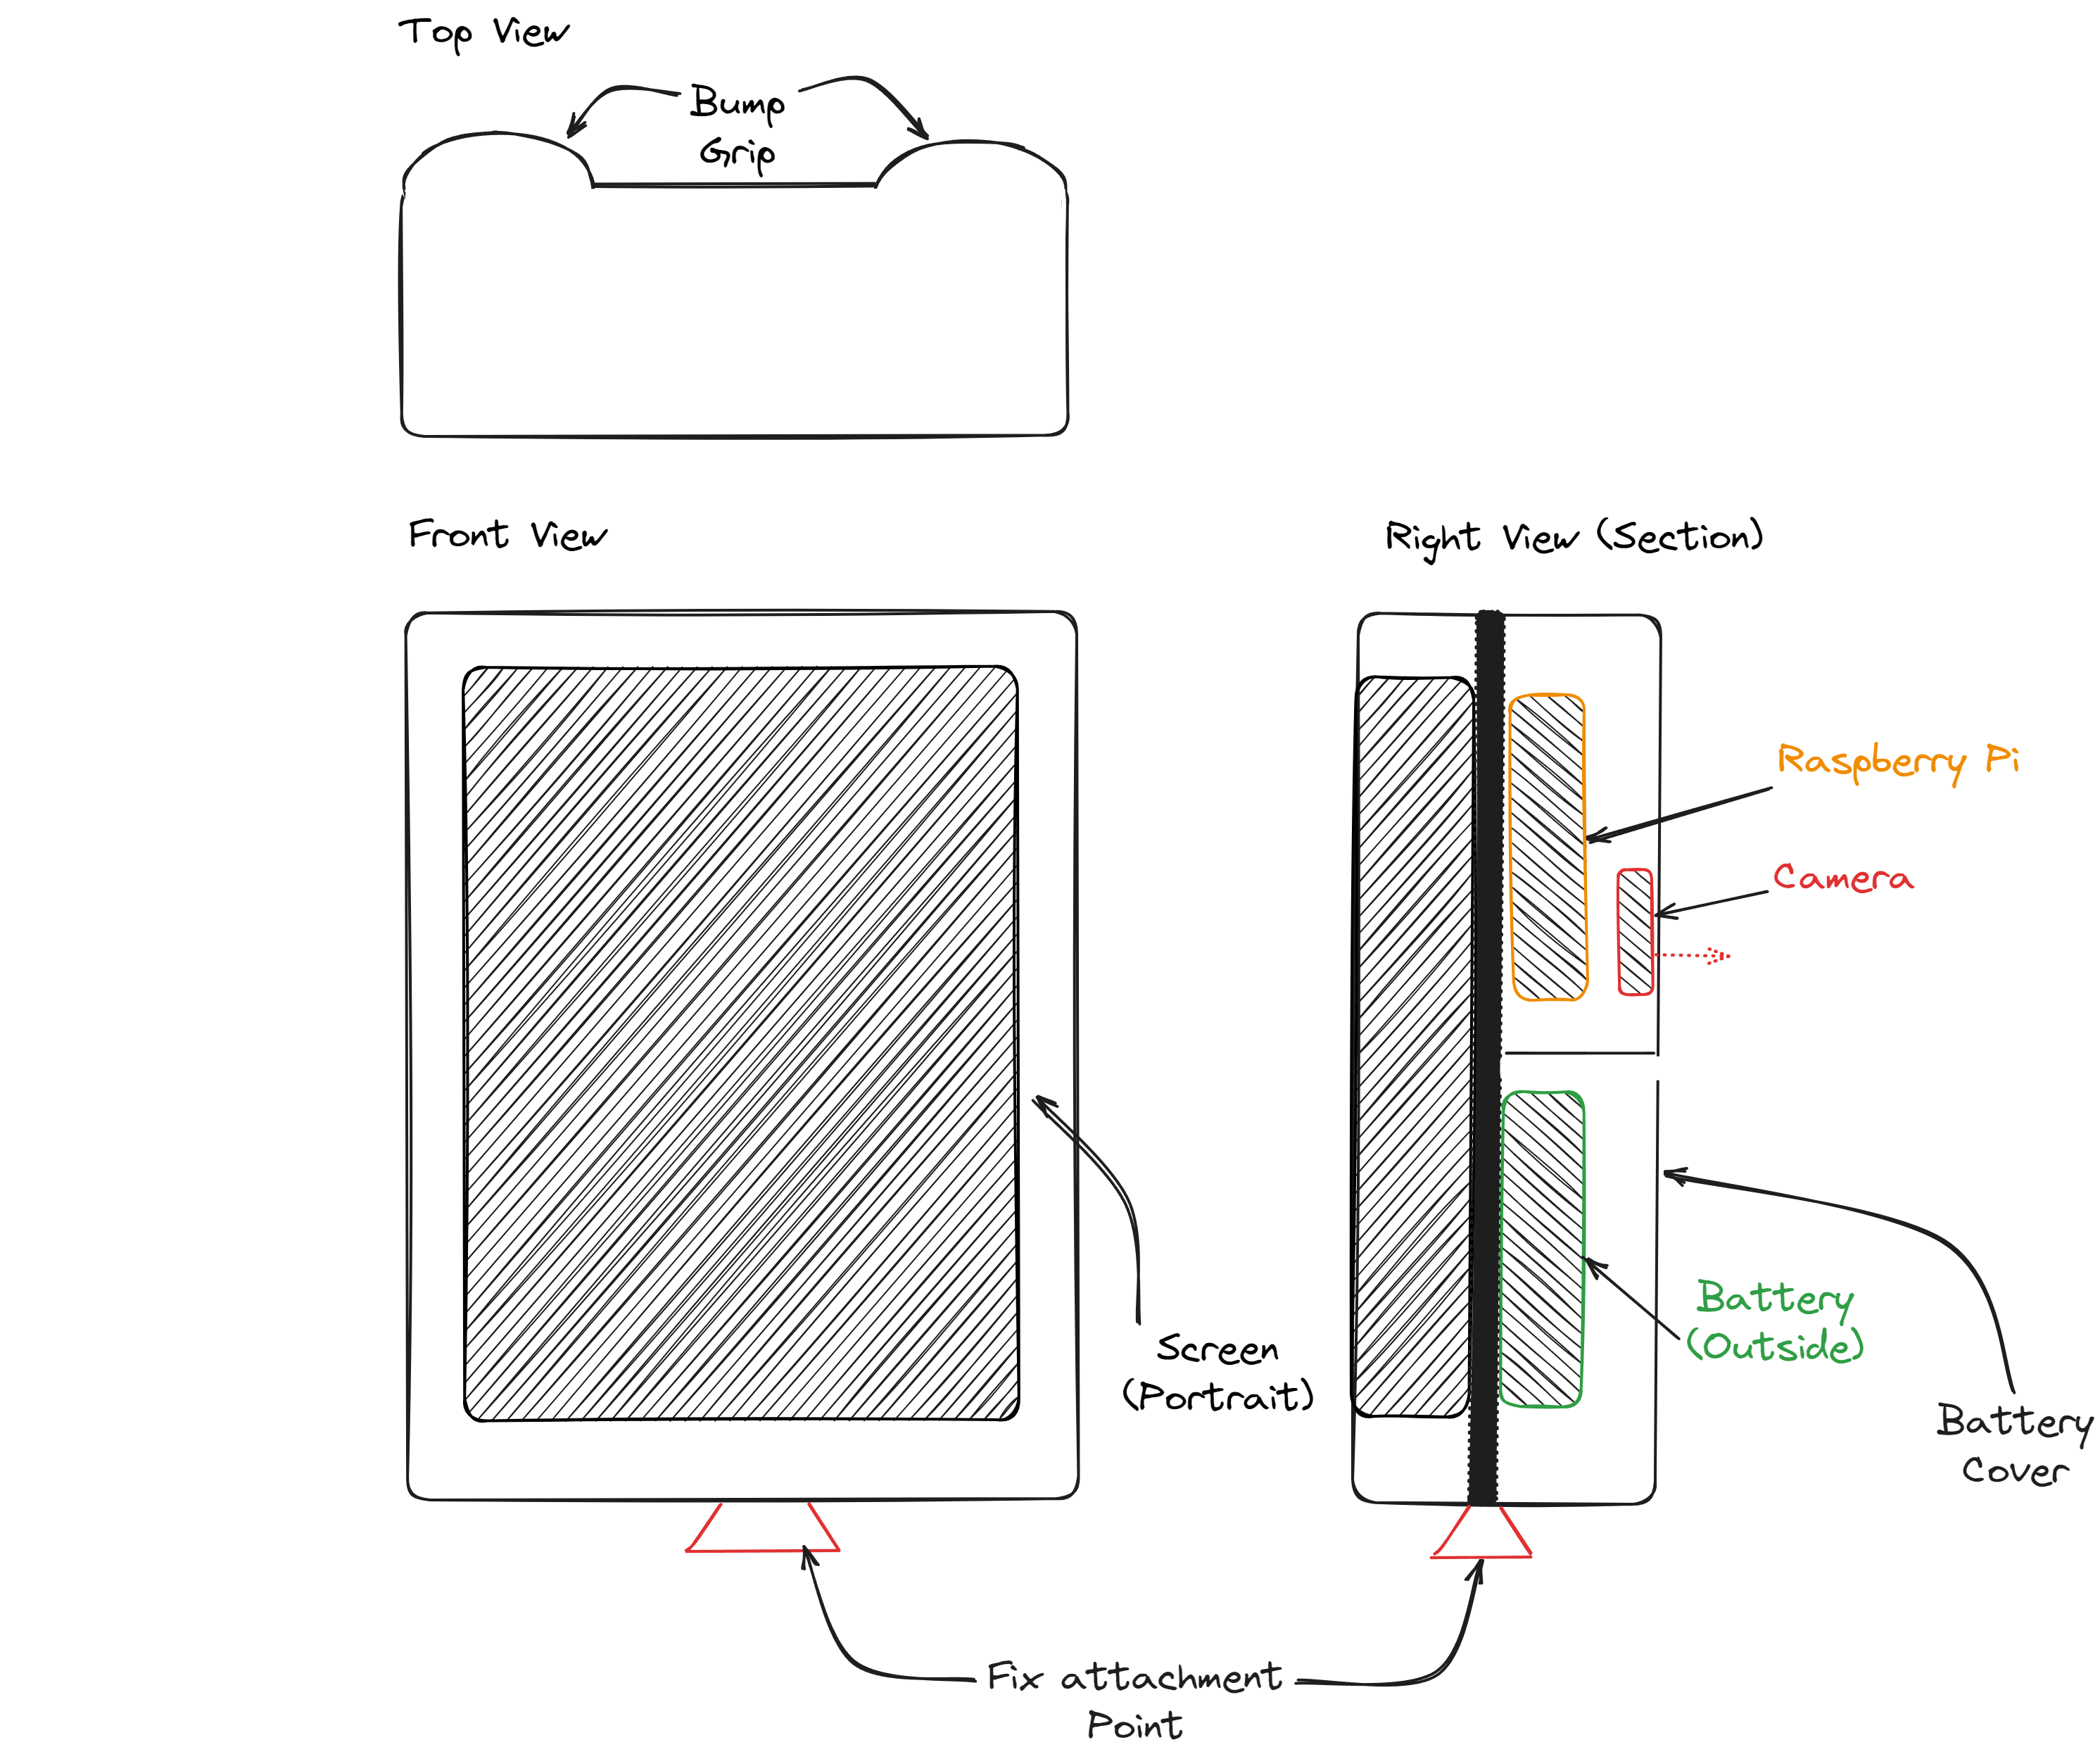
\includegraphics[width=0.75\linewidth]{texs/Part1/chapter3/image/v3.png}
    \caption{Sketch of Solution Variant 3}
    \label{fig:sketch-solution-variant-3}
\end{figure}

\subsection{Solution Variant 4}
Solution Variant 4 copies many features from Solution Variant 3, but with one significant change in the body type. Solution Variant 4 opts for a more minimalistic skeleton design, which results in a lightweight yet adequately supportive body for the internal components.

\begin{figure}[H]
    \centering
    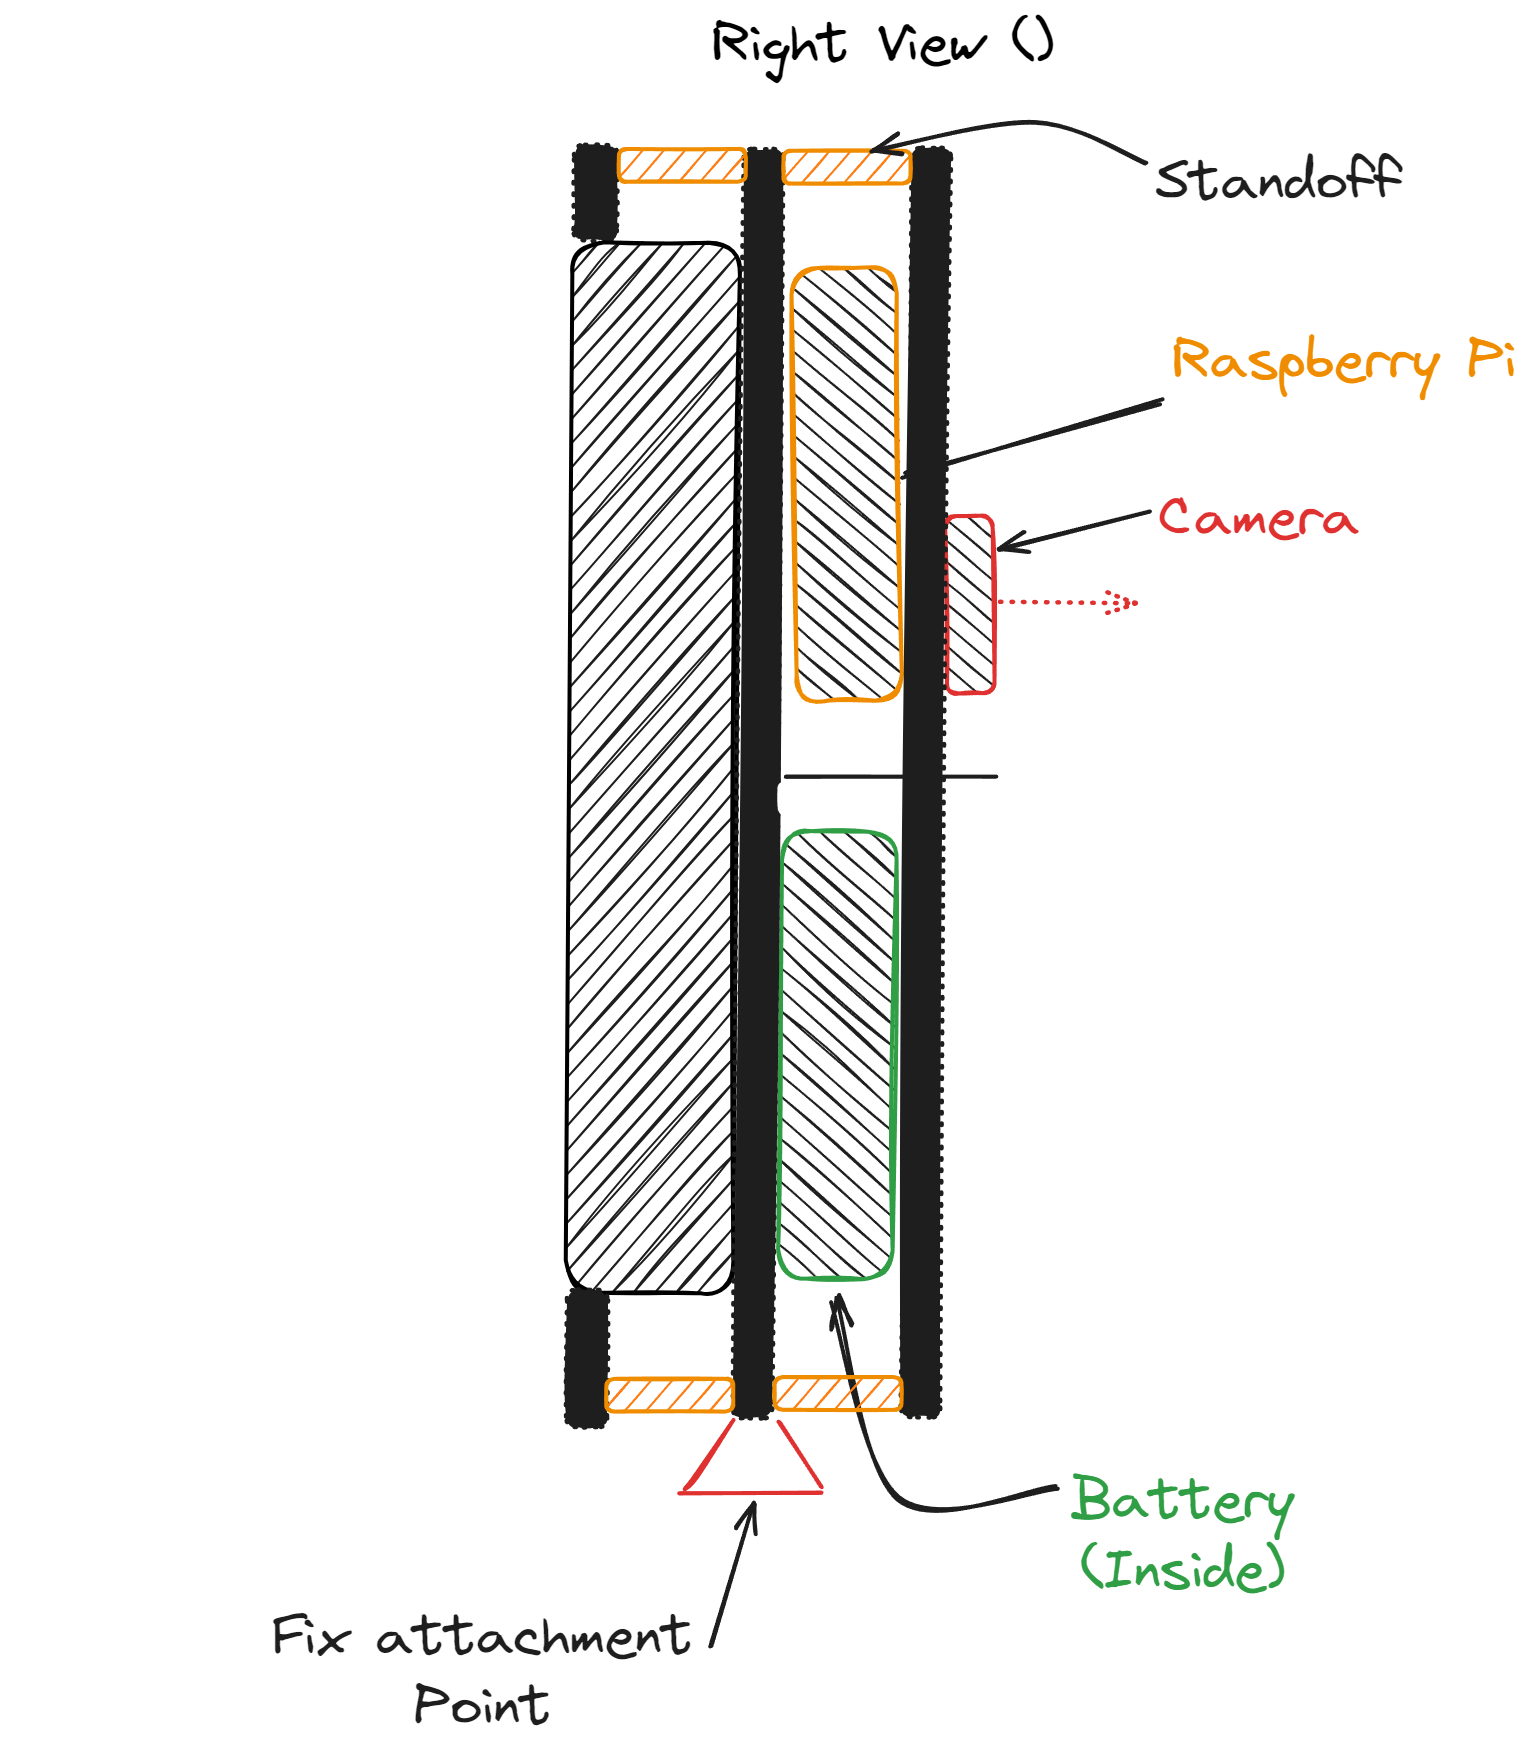
\includegraphics[width=0.5\linewidth]{texs/Part1/chapter3/image/v4.png}
    \caption{Sketch of Solution Variant 4}
    \label{fig:sketch-solution-variant-4}
\end{figure}

\subsection{Solution Variant 5}
Solution Variant 5 introduces a unique design approach, deviating from the tablet-like structure seen in previous solutions. Instead, it adopts a Point of Service-like component placement, where the Raspberry Pi, Battery, Camera, and Screen are configured in a distinctive layout. The screen is positioned at an angle, differentiating it from the previous variants.

Regarding screen orientation, Solution Variant 5 retains a portrait mode, which can be advantageous in scenarios requiring vertical displays. The device is designed for body grip handling, offering a secure way to hold and interact with the device.

A notable difference is the external AAA battery setup, which enhances convenience by offering easy battery replacement and compatibility with standard batteries. The body structure follows the familiar sandwich-type design, providing robust protection for the internal components.

For mounting purposes, Solution Variant 5 utilizes the detachable tripod system, enabling seamless attachment and detachment from a tripod stand. Like its predecessors, it relies on a touch screen as the primary control mechanism, ensuring intuitive user interactions.

\begin{figure}[H]
    \centering
    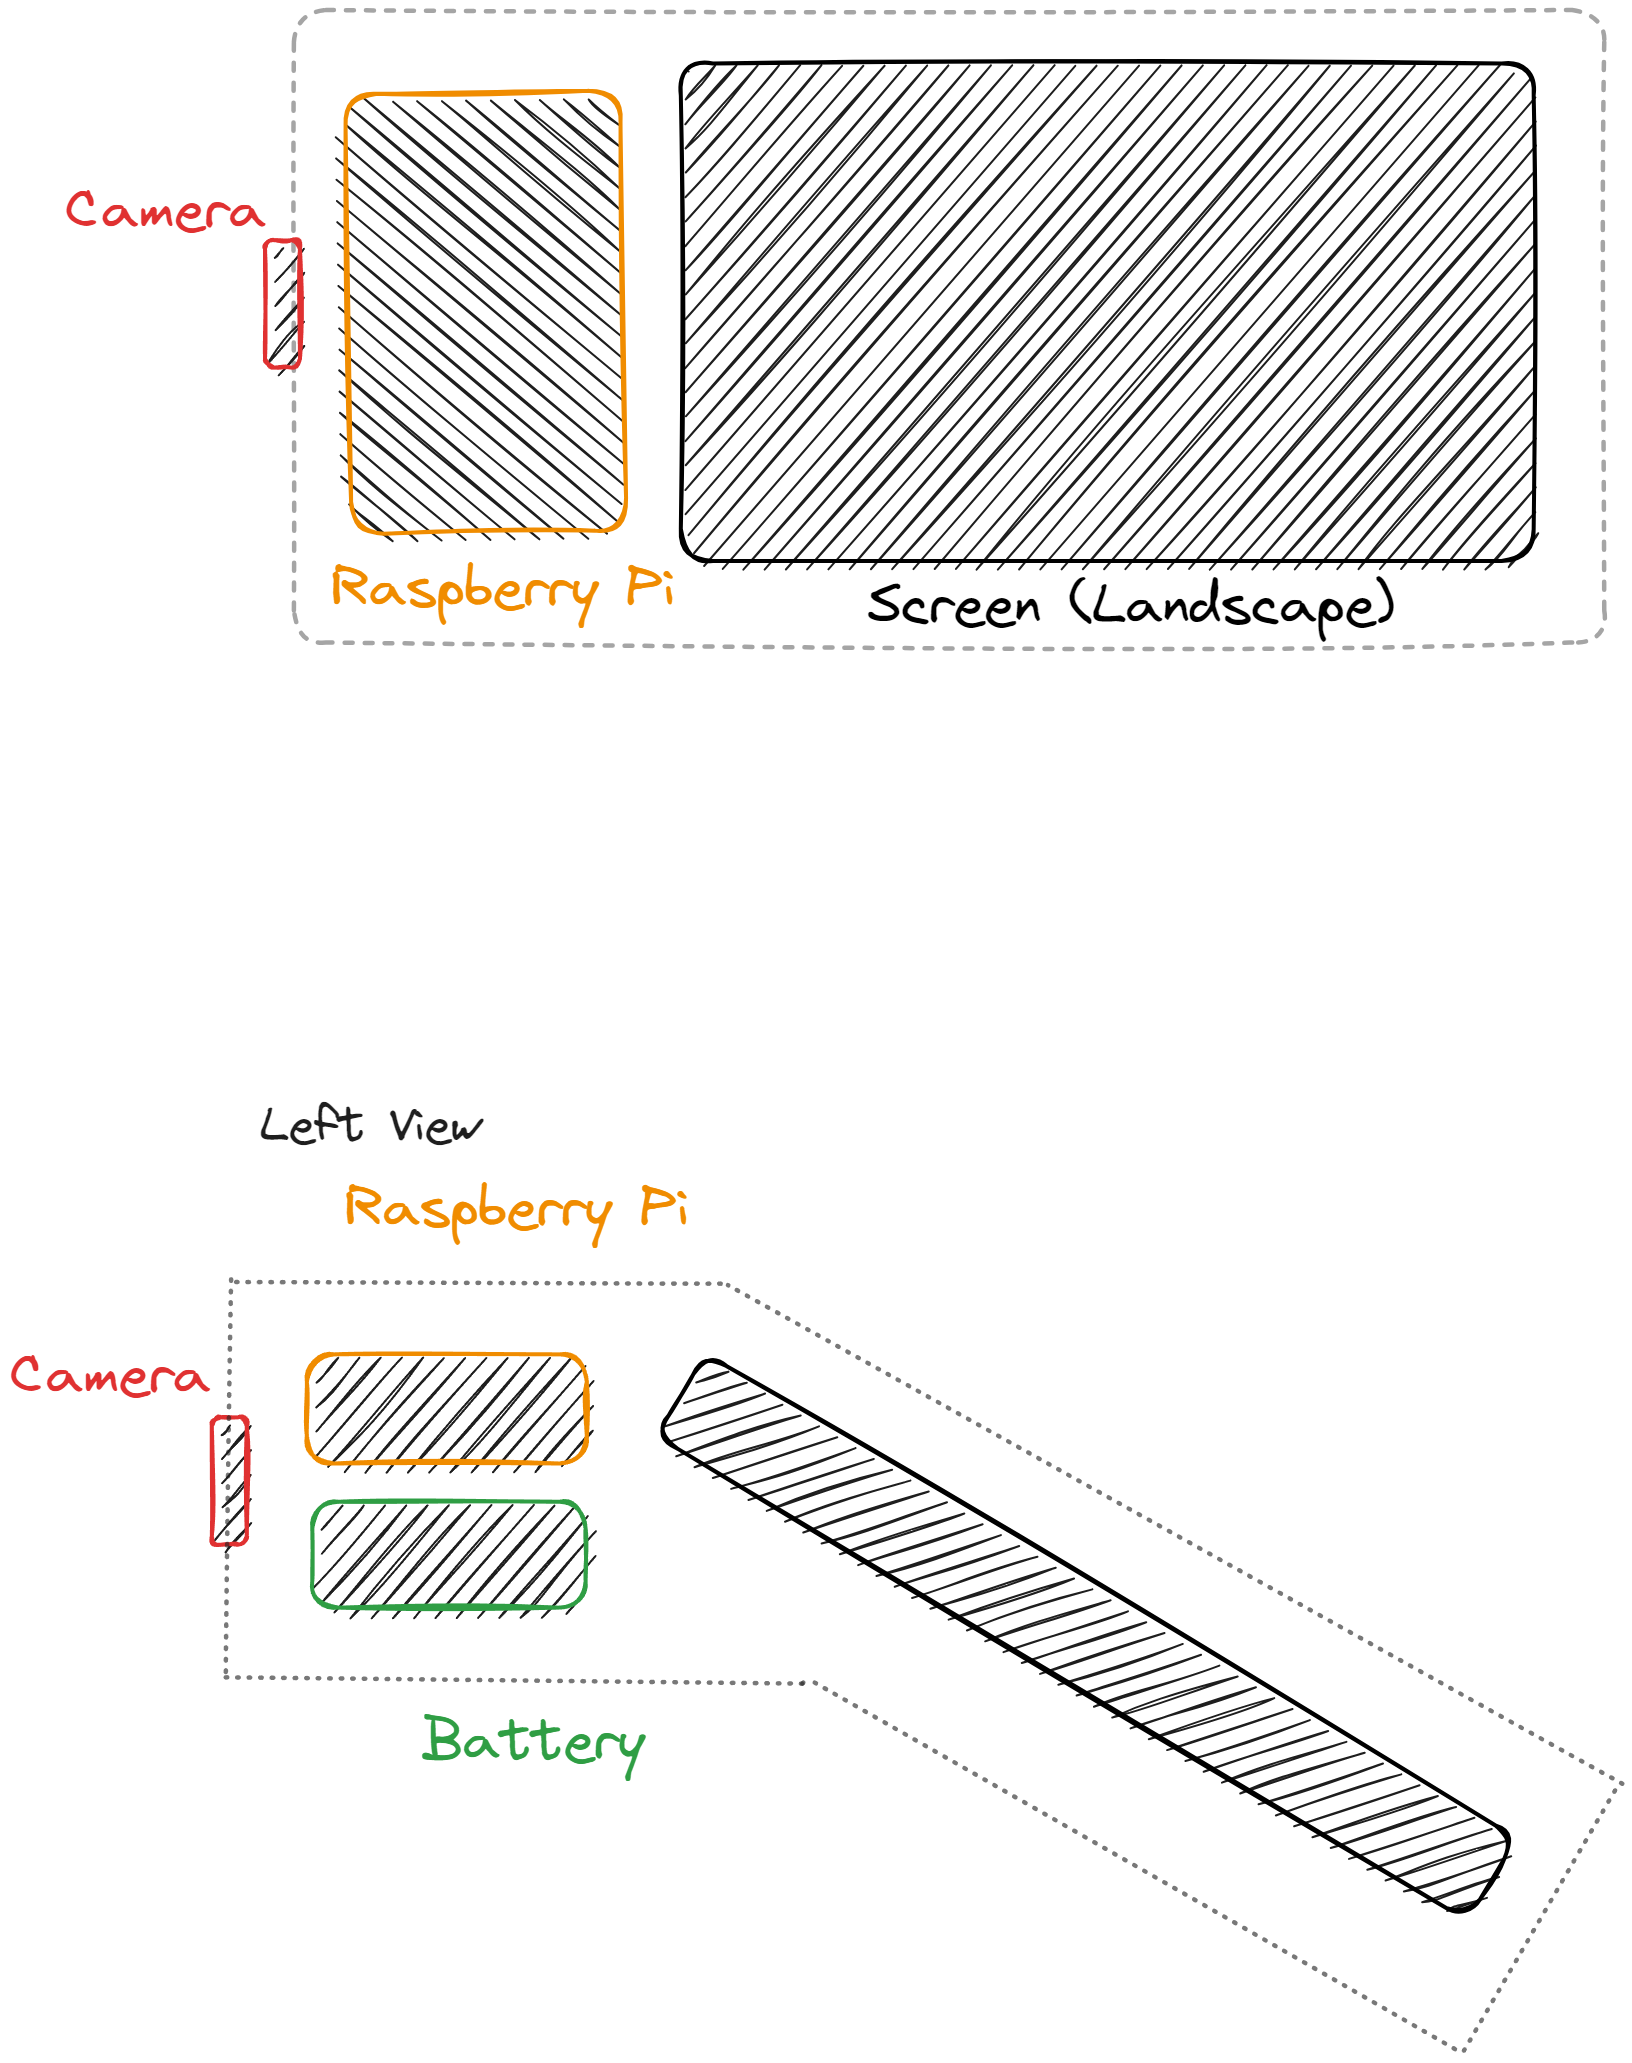
\includegraphics[width=0.5\linewidth]{texs/Part1/chapter3/image/v5.png}
    \caption{Sketch of Solution Variant 5}
    \label{fig:sketch-solution-variant-5}
\end{figure}

\subsection{Solution Variant 6}
Solution Variant 6 closely mirrors Solution Variant 5 regarding component placement and screen orientation. This variant, too, adopts the Point of Service-like layout with a portrait screen orientation. However, it introduces a pistol handle for handling, providing a firm and ergonomic grip for users.

The battery is positioned externally, offering the same benefits of easy battery replacement and extended usage periods. Regarding body design, Solution Variant 6 employs a bowl-like structure with all components attached to the main body. This design choice provides protection and enclosure while reducing overall weight.

The detachable tripod system is employed for mounting, ensuring compatibility with tripod stands. As with previous variants, the control mechanism relies on the touch screen for user interactions.

\begin{figure}[H]
    \centering
    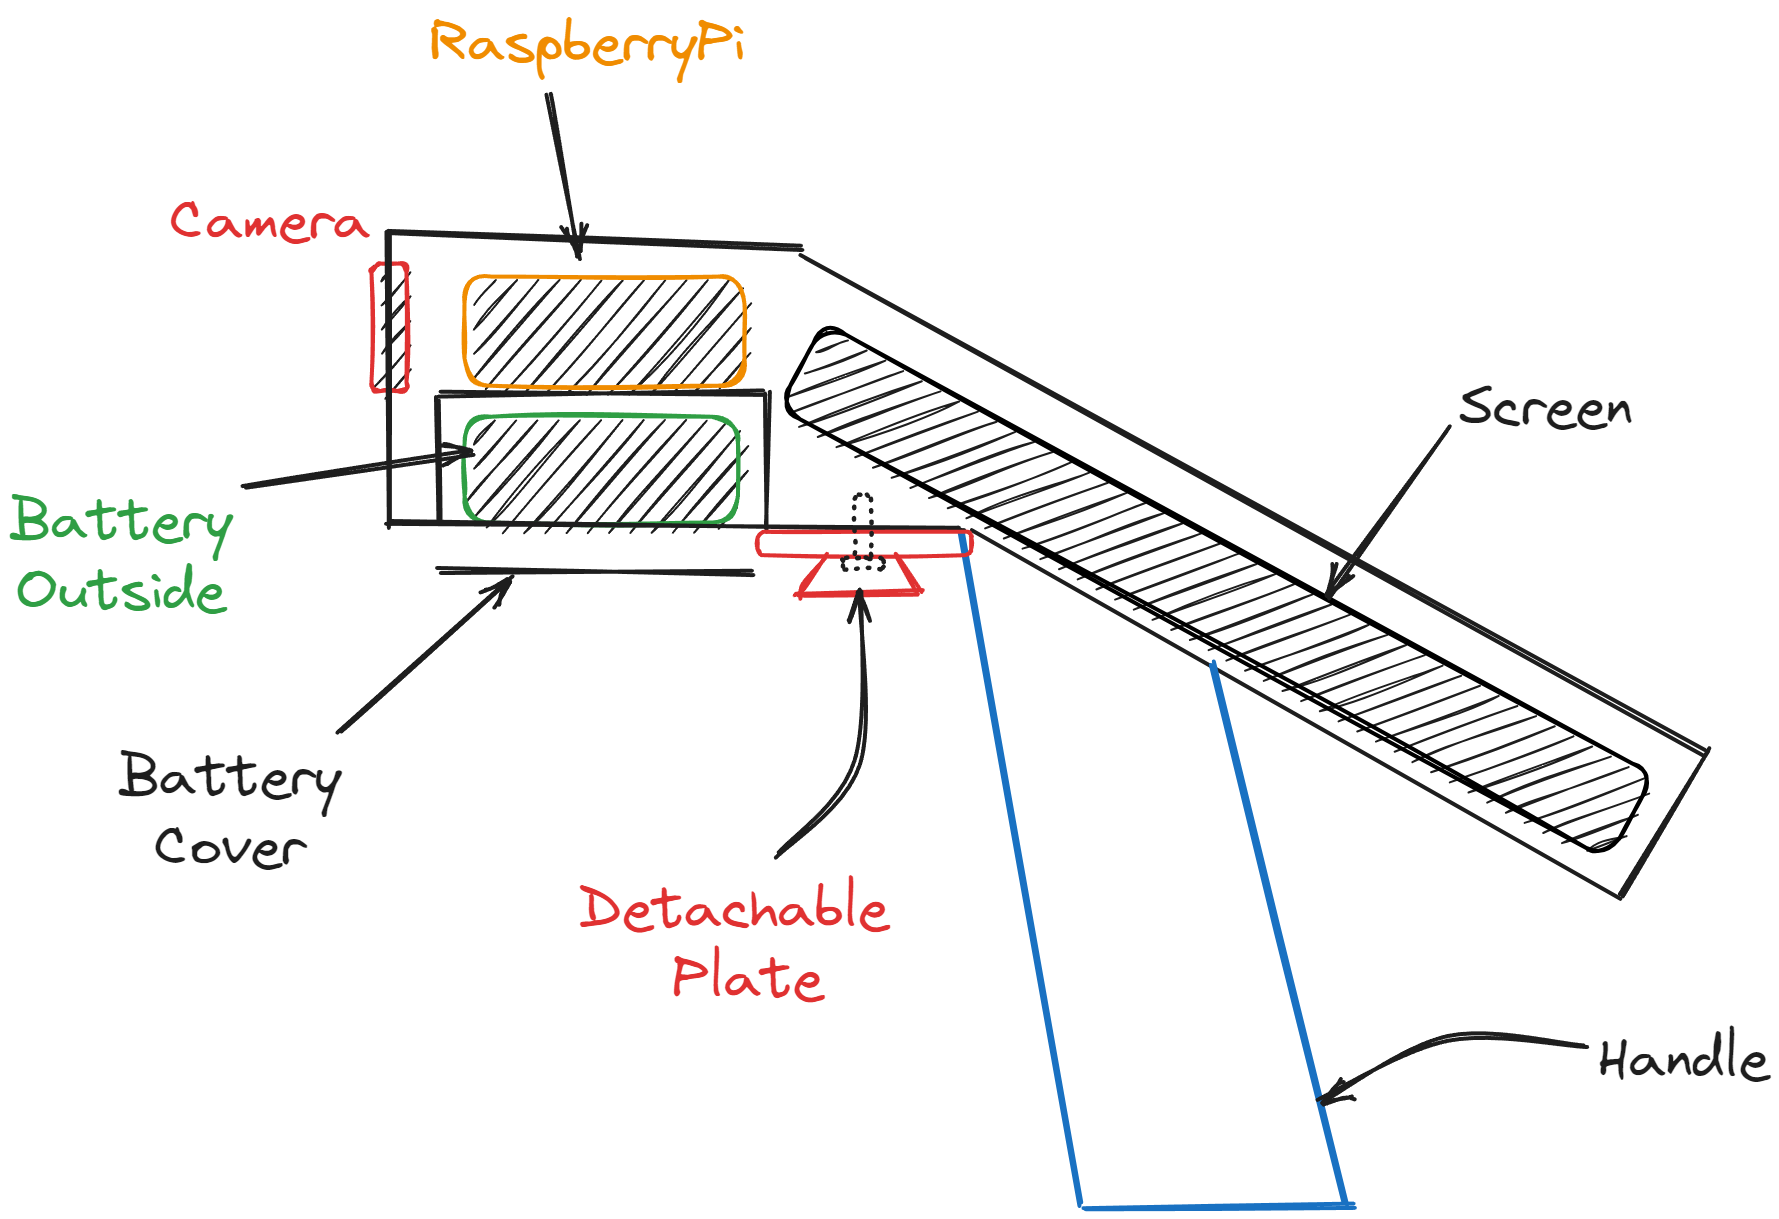
\includegraphics[width=0.5\linewidth]{texs/Part1/chapter3/image/v6.png}
    \caption{Sketch of Solution Variant 6}
    \label{fig:sketch-solution-variant-6}
\end{figure}

\subsection{Solution Variant 7}
In Solution Variant 7, a distinct design approach with a Handheld PC-like component placement is produced. This configuration aligns the screen and battery, positioning the Raspberry Pi behind the screen.

The screen orientation is in landscape mode, offering a broader horizontal display view. The device is designed with a bump grip for secure and comfortable handling. Notably, the battery is placed internally and utilizes a battery pack, contributing to an integrated and seamless appearance.

The chassis structure adopts a bowl-like design, ensuring secure enclosure and protection for all components. The device incorporates a built-in tripod system for mounting, providing a stable attachment to a tripod stand.

Solution Variant 7 combines a touch screen and physical buttons as the control mechanism. This dual-input approach provides users multiple options for interacting with the device's functionalities, enhancing versatility and usability in various scenarios.

\begin{figure}[H]
    \centering
    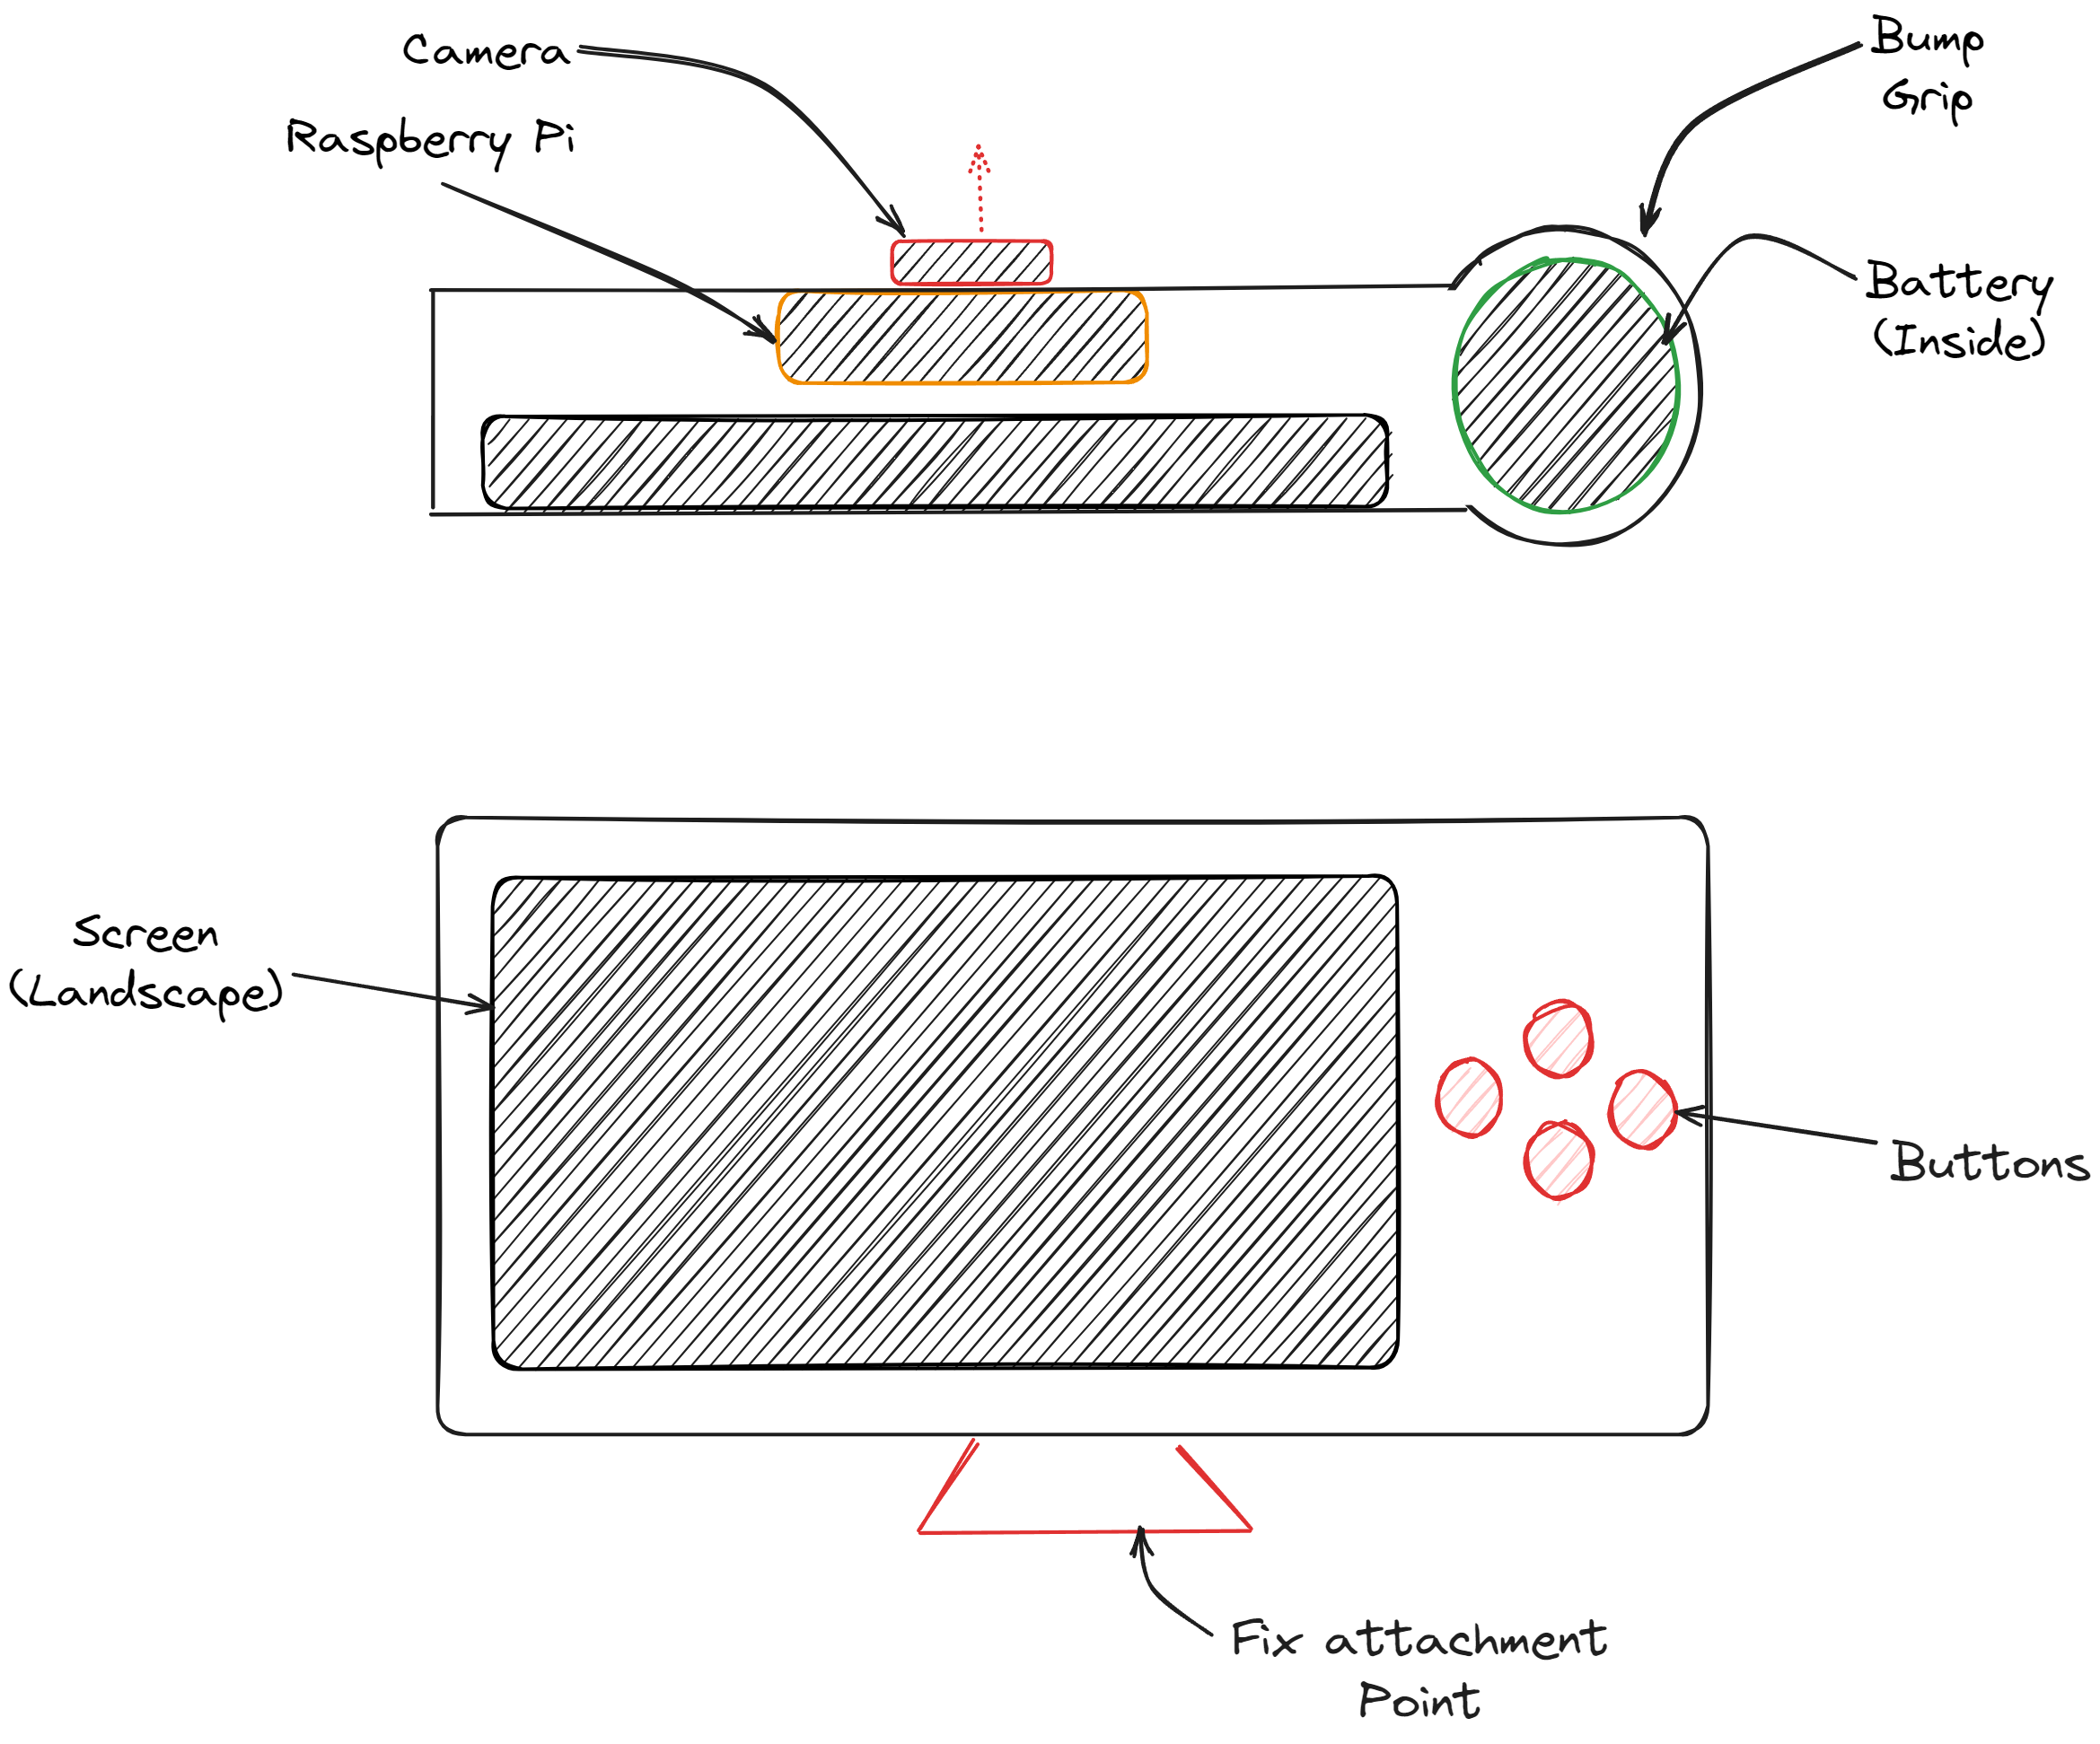
\includegraphics[width=0.5\linewidth]{texs/Part1/chapter3/image/v7.png}
    \caption{Sketch of Solution Variant 7}
    \label{fig:sketch-solution-variant-7}
\end{figure}

\subsection{Solution Variant 8}
Solution Variant 8 features a Camcorder-like component placement. The Raspberry Pi, Battery, Camera, and Screen are arranged similarly to a camcorder, with the screen positioned at a hinge, allowing it to change angles for flexible viewing.

The screen orientation remains landscape, providing a broad horizontal display view. The device is designed with a body grip for secure and comfortable handling. The battery is placed internally, and a power bank is used to provide a reliable power source.

The chassis structure follows a bowl-like design, offering protection and sturdiness for the internal components. A fixed-mount tripod system is employed for mounting purposes, providing stability and ease of use when attaching the device to a tripod stand.

As with some of the previous variants, Solution Variant 8 combines both a touch screen and physical buttons as the control mechanism, offering users the flexibility to interact.

\begin{figure}[H]
    \centering
    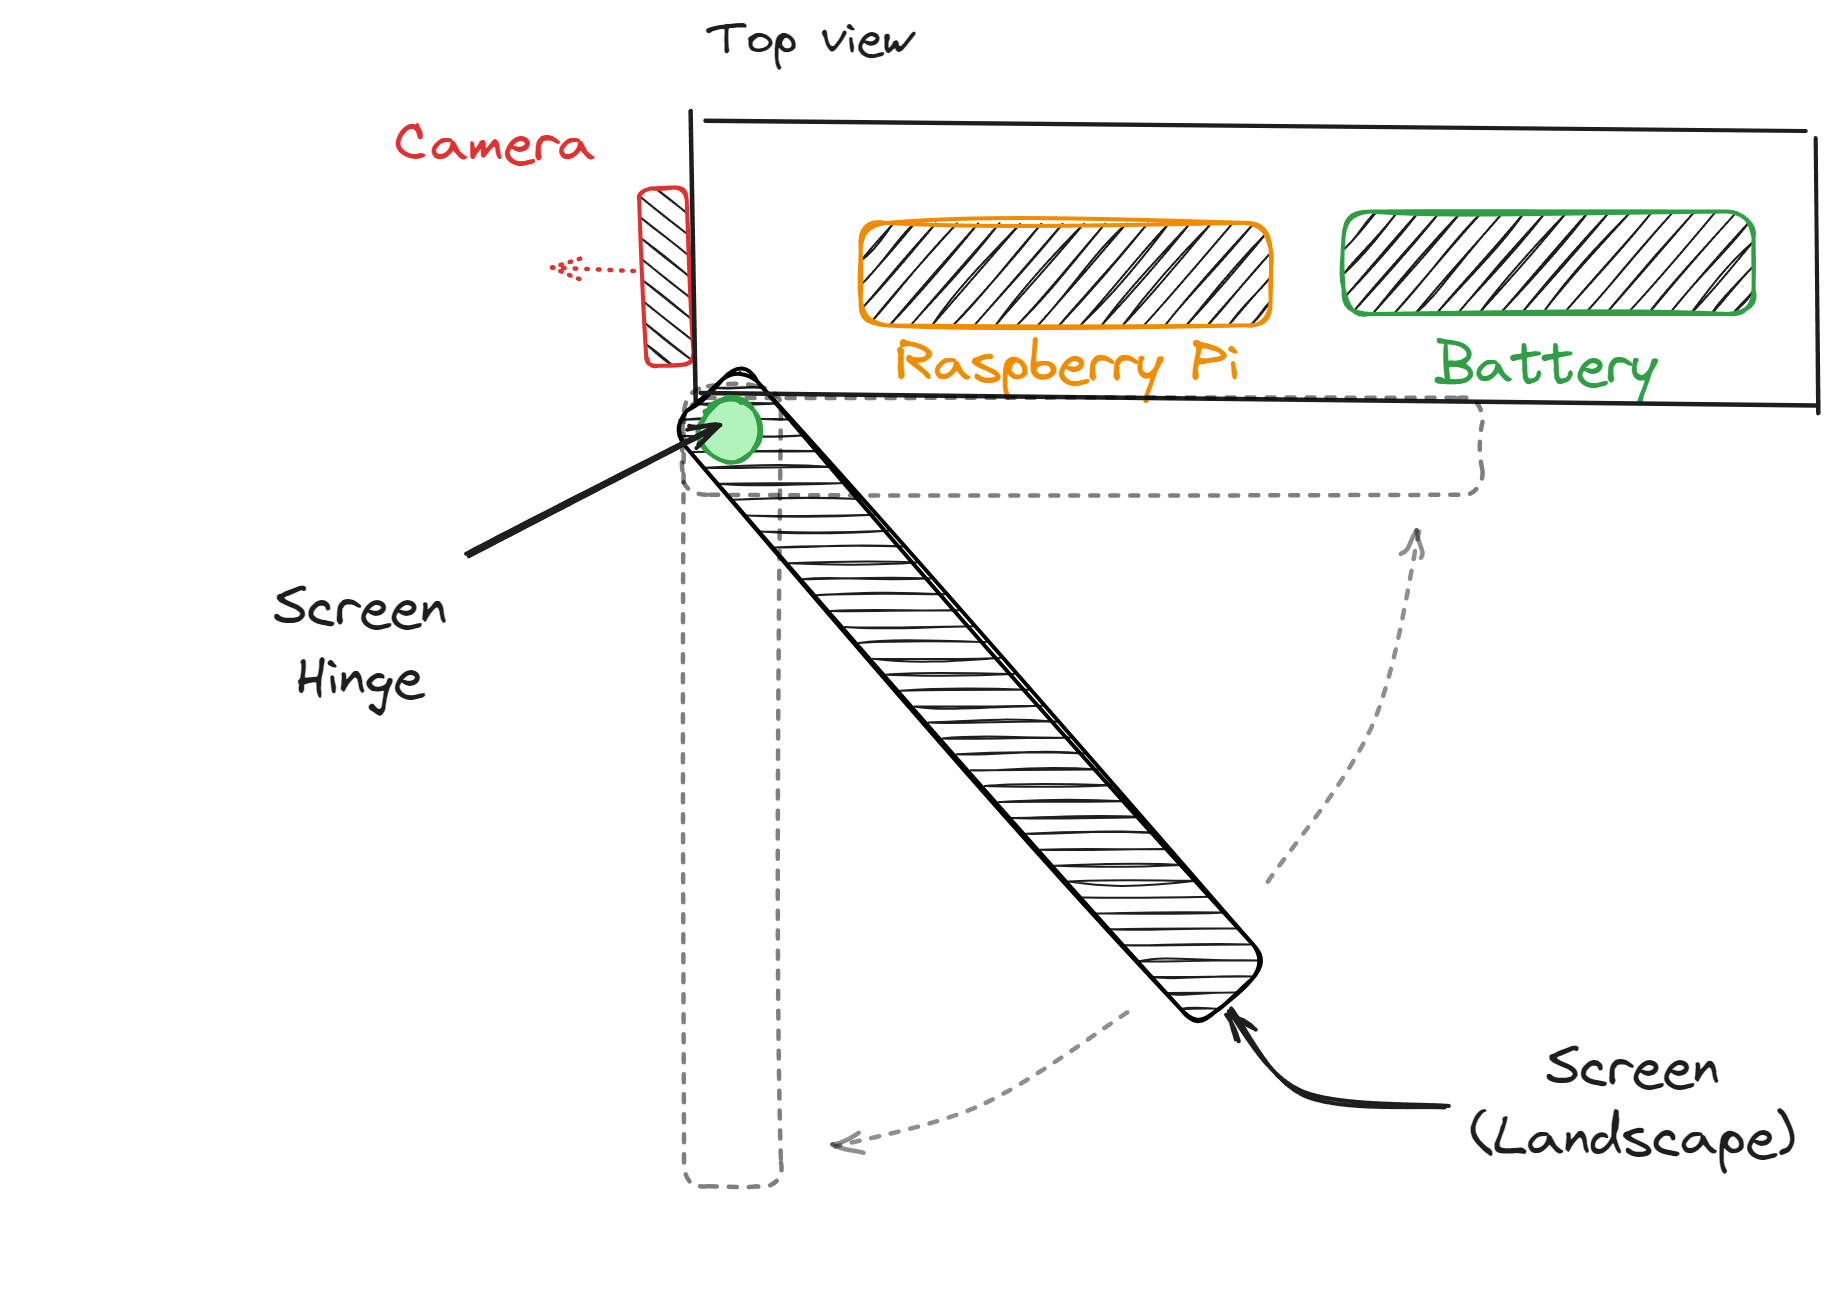
\includegraphics[width=0.5\linewidth]{texs/Part1/chapter3/image/v8.png}
    \caption{Sketch of Solution Variant 8}
    \label{fig:sketch-solution-variant-8}
\end{figure}

\section{Filtering of Solution Variants}
\label{sec:filtering-of-solution-variants}
As shown in Figure \ref{fig:morphological-chart-with-solution-variants}, multiple solution variants were generated. However, not all of these solutions are feasible and practical. As advised by Pahl and Beitz \cite{Pahl07s}, it is necessary to reduce the vast number of theoretically possible but practically unachievable solutions as early as possible. However, caution should be exercised not to discard valuable working principles, as they often play a crucial role in forming a favorable and effective working structure when combined with others.

Additionally, Pahl and Beitz \cite{Pahl07s} suggest a method that can be used to filter the solution variants. This method is known as the selection chart, which consists of two steps: elimination and preference. Initially, all clearly unsuitable proposals are removed. If a substantial number of solutions remain, preference is given to those who stand out as markedly superior. Only these preferred solutions are evaluated during the final stages of the conceptual design phase.

Pahl and Beitz suggest the following criteria for eliminating unsuitable solutions:
\begin{itemize}
    \item \textbf{Criteria A:} Compatible with the overall task
    \item \textbf{Criteria B:} Fulfill demands of requirement list
    \item \textbf{Criteria C:} Realisable in principle
    \item \textbf{Criteria D:} Within permissible cost
\end{itemize}

These criteria are applied step by step to examine each solution. If any of the exclusion criteria are not met, the solution is rejected, and further criteria are not assessed. Additionally to the exclusion criteria, the following preference criteria are used to prioritize the remaining solutions:

\begin{itemize}
    \item \textbf{Criteria E:} Incorporates direct safety measures
    \item \textbf{Criteria F:} Preferred by the designer
\end{itemize}

Criteria E and F are then used to prioritize solutions if there are still too many options after the initial screening. The remarks column provides explanations for excluding or favoring each solution. The final assessment of the functional principles is recorded in the rightmost column of the selection list.

\begin{figure}[ht!]
    \centering
    {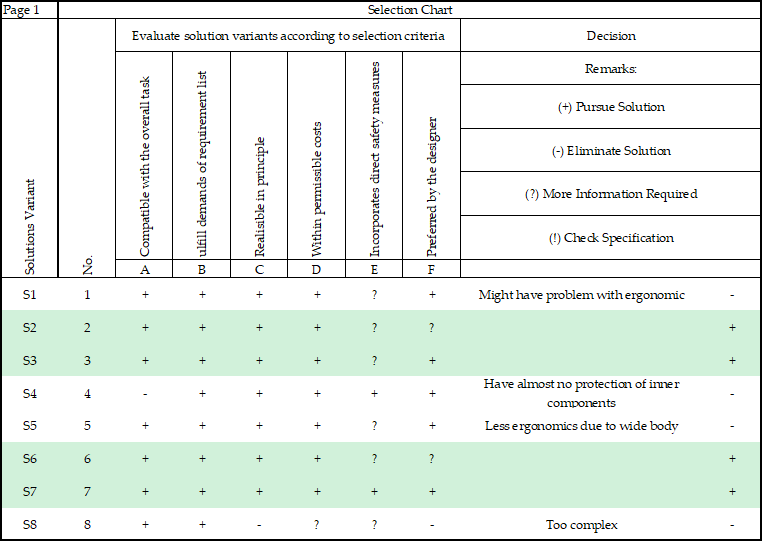
\includegraphics[width=\linewidth]{texs/Part1/chapter3/image/selchart2.png}}
    \caption{Selection Chart for Solution Variants}
    \label{fig:selection-chart-solution-variants}
\end{figure}

The result of the selection chart, as shown in Figure \ref{fig:selection-chart-solution-variants}, indicates that solutions S1, S4, S5, and S8 have been eliminated and will not be considered for the next stage of the design process.


\chapter{Embodiment Design}
The next phase in the design methodology is embodiment design. This phase, as defined by Pahl and Beitz \cite{Pahl07t}, involves starting with the fundamental solution or concept for a technical product and then advancing the design in alignment with technical and economic criteria, taking into account further information. The ultimate objective is to reach a stage where the subsequent detailed design can smoothly progress into the production phase.
Figure \ref{fig:embodiment_design} shows the steps involved in this phase.

\begin{figure}
    \centering
    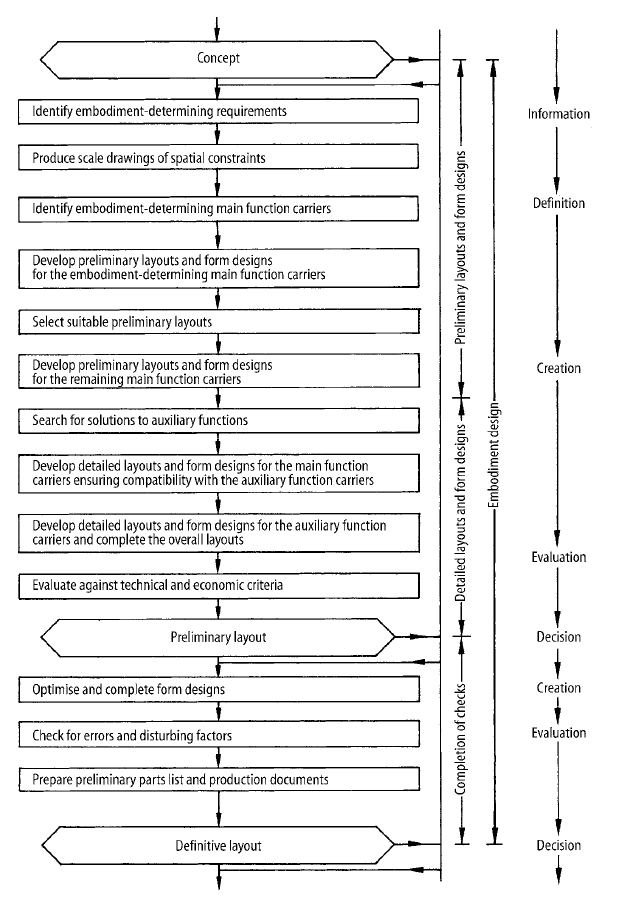
\includegraphics[width=0.92\linewidth]{texs/Part1/chapter4/image/embodiment.png}
    \caption{Steps in Embodiment Design \cite{Pahl07u}}
    \label{fig:embodiment_design}
\end{figure}

\section{Basic Rules of Embodiment Design}
When it comes to product design, there are some basic rules that must be followed. As defined by Pahl and Beitz \cite{Pahl07v}, they include clarity, simplicity, and safety. Neglecting these rules can potentially result in issues and accidents. Subsequent sections will provide a comprehensive exploration of these guidelines.

\subsection{Clarity}
Clarity, as described by Pahl and Beitz \cite{Pahl07w}, entails establishing clear and unambiguous connections within a design. This involves ensuring straightforward relationships between subfunctions, inputs, and outputs to prevent any confusion or misinterpretation. It also extends to the selection of a working principle, where designers should choose principles that clarify cause-and-effect dynamics, align with the product's purpose, and optimize its layout by eliminating unnecessary complexity.

Additionally, clarity applies to the broader design structure, whether it involves multiple working principles or component combinations. It mandates that the design facilitates the orderly flow of energy, materials, and signals, preventing adverse effects like excessive forces or wear. This commitment to clarity ultimately enhances the product's reliability and durability.

\subsection{Simplicity}
Simplicity \cite{Pahl07x} in design is epitomized by an uncomplicated and easily comprehensible approach, often achievable by using fewer components. Such simplicity can lead to cost savings, reduced wear and tear, and minimized maintenance requirements. Nonetheless, it's crucial to strike a balance, as certain functions inherently demand a minimum number of components.

Designers should, therefore, strive for a minimalist approach by employing the fewest components possible while maintaining straightforward shapes, as this promotes efficiency and practicality in the design process. The choice between numerous components with simple shapes, albeit potentially increasing production effort, and a single, more affordable cast component should be made while considering the specific problem and constraints.

\subsection{Safety}
Safety \cite{Pahl07y} considerations are crucial in ensuring both the effective performance of technical functions and the protection of people and the environment. Designers rely on a safety methodology outlined in the German industry standard DIN 31 000, which encompasses three levels: direct safety, indirect safety, and warnings. In general, designers should prioritize direct safety measures, seeking solutions that inherently eliminate potential dangers. Only when this is not feasible should they resort to indirect safety measures, involving the construction of specialized protective systems.

Warnings, which serve to highlight dangers and hazard zones, are best utilized in conjunction with direct and indirect safety measures, clarifying specific risks. As designers address technical challenges, they encounter various constraints, not all of which can be simultaneously overcome. However, their objective remains to develop solutions that come as close as possible to meeting all requirements. It's important to note that exceptionally high safety demands can complicate design, potentially diminishing clarity and economic viability, and even leading to project abandonment in some cases.

\section{Guideline of Embodiment Design}
In addition the the basic rules of embodiment design, Pahl and Beitz \cite{Pahl07z} also stress the importance of following a set of design guidelines to help designers meet the specific requirements and constraints. For this project, the following design guidelines are considered:

\begin{itemize}
    \item Design for production
    \item Design for ergonomics
\end{itemize}

\subsection{Design for Production}
Design for production \cite{Pahl07aa} is a design guideline that emphasizes the importance of considering the production process during the design phase. This approach enables designers to optimize the production cost and times while ensuring the product's functionality and quality. By following the basic rules of clarity and simplicity, designers are already on the right track to achieving this goal.

\subsubsection{Appropriate Overall Layout Design}
Overall layout design, derived from the function structure, influences product division into assemblies and components, including sourcing decisions (in-house, bought-out, standard parts), production procedures, dimensions, batch sizes, joining methods, and quality control.

The layout can lead to differential, integral, composite, or building-block construction methods. Differential Construction involves breaking down components into easily produced parts, facilitating adaptability, increased component batch sizes, and easier quality assurance. However, it demands greater machining and assembly costs and may have functional limitations due to joints.

Integral Construction combines multiple parts into a single component, reducing costs due to integration but can be complex and sensitive to market conditions. Composite Construction involves connecting different parts requiring further work, applying multiple joining methods or using various materials for optimal property utilization.

Building Block Construction results from splitting components so that the parts or assemblies can be used in other products or variants, offering flexibility and cost savings. These construction methods offer specific advantages and disadvantages, depending on the context and design requirements.

\subsubsection{Appropriate Form Design of Components}
During component form design, designers significantly impact production costs, times, and product quality by choosing shapes, dimensions, surface finishes, tolerances, and fits. These choices influence production procedures, machine types, in-house vs. bought-out components, materials, and quality control procedures.

Conversely, production facilities influence design features, which may include dimension limitations necessitating component division or the acquisition of bought-out components. Many guidelines exist for appropriate component form design, and tolerances are crucial.
Figure \ref{fig:guideline} shows the design guidelines for designing components specifically for 3D printing.

\begin{figure}
    \centering
    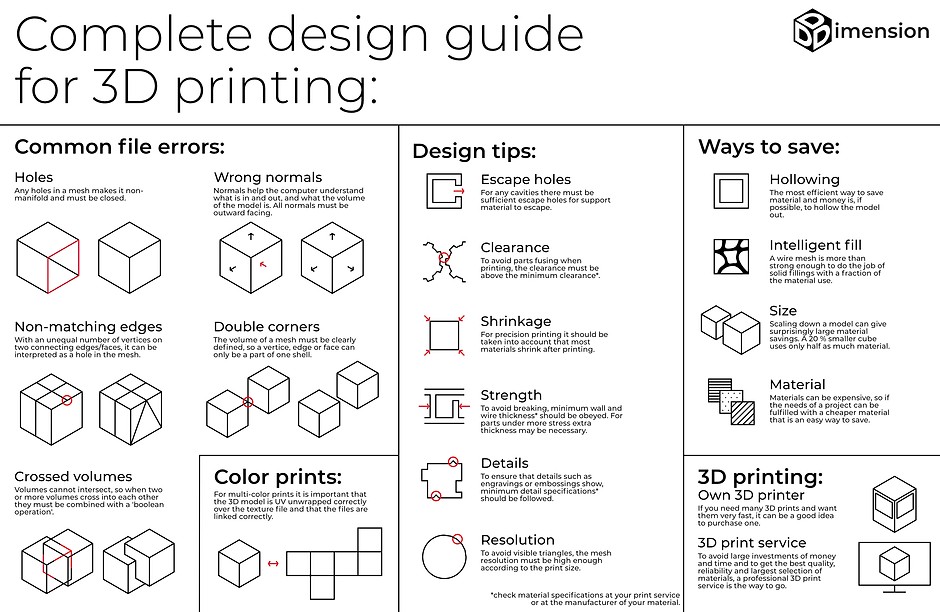
\includegraphics[width=0.92\linewidth]{texs/Part1/chapter4/image/guidelines.png}
    \caption{Design guidelines for 3D printing \cite{DDDimension_22}}
    \label{fig:guideline}
\end{figure}

\subsection{Design for Ergonomics}
Ergonomics \cite{Pahl07ab} is vital in designing technical products, aiming to align them with human characteristics, needs, and interfaces. It covers a broad range of items, including everyday household products and human-machine interfaces. Recent focus has shifted to user-friendly interfaces and ergonomic workplace assessment tools.

Ergonomic design considers various factors, starting with biomechanics, which addresses how body postures and movements interact with product design. Physiological aspects, such as muscle action, circulation, and temperature regulation, are crucial. Sensory factors like light and noise must also be taken into account. Psychological aspects guide design to minimize cognitive load and enhance user-friendliness.

Ergonomics extends to active and passive user involvement. Active involvement necessitates careful planning, assessing if human interaction is necessary and effective. Passive involvement addresses how users are affected by products, considering factors like energy flows, vibrations, light, climate, and noise.

Identifying ergonomic requirements can follow two approaches. The object-based approach is used when designing predefined systems or products, employing checklists tailored to specific items. The effect-based approach applies to new situations, analyzing the effects of energy, material, and signal flows, ensuring they meet ergonomic requirements. Both aim to prioritize user comfort, safety, and efficiency while minimizing discomfort and errors.

\section{Preliminary Design}
In this section, we will explore multiple designs for the device. These designs are detailed 3D models of the device that we will use to evaluate their respective designs and assess their feasibility. Each of these preliminary designs will be based on the selected solution from the previous phase. Alongside the models, we will also present the production costs for each of these designs. For a more detailed breakdown of the production costs, please refer to Appendix \ref{appendix:production_cost}.


\subsection{Preliminary Design Variant 2}
\label{subsec:preliminary_design_variant_2}
In this section, we present a comprehensive design overview of Solution Variant 2. Figure \ref{fig:preliminary_design_variant_2} showcases the 3D model of Variant 2, while Figure \ref{fig:variant2_views} provides various perspectives and body measurements of the device. The key emphasis of this design is its ergonomic shape and user-friendly attributes. With a thickness of 49.2 mm (Figure \ref{fig:variant2_right_view}), it successfully strikes a balance between being slim and accommodating essential components for optimal performance.

\begin{figure}[h!]
    \centering
    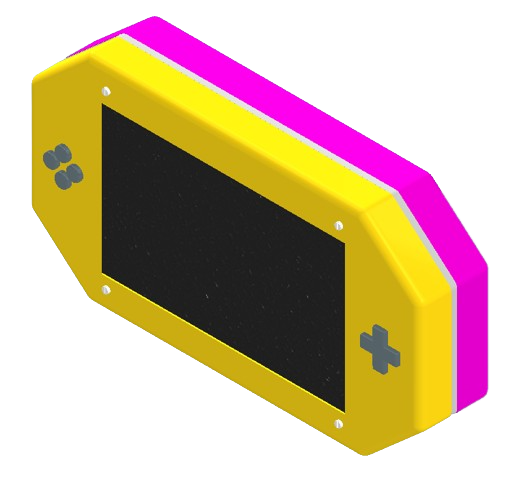
\includegraphics[height=5 cm]{texs/Part1/chapter4/image/v21.png}
    \caption{Preliminary Design Variant 2}
    \label{fig:preliminary_design_variant_2}
\end{figure}

\begin{figure}[h!]
    \centering
    \begin{subfigure}[c]{0.65\textwidth}
        \begin{minipage}{\textwidth}
            \centering
            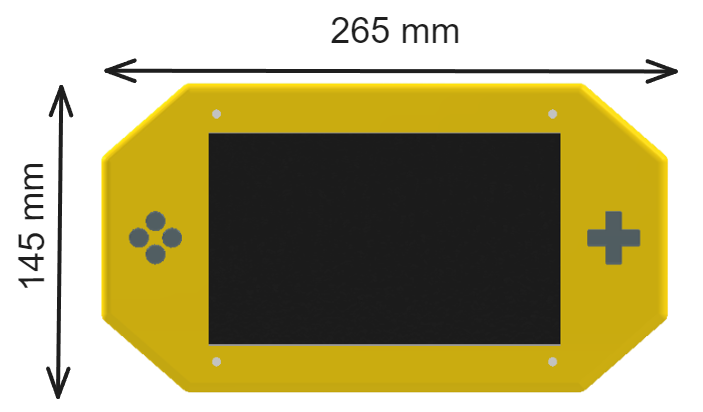
\includegraphics[height=4 cm]{texs/Part1/chapter4/image/v22.png}
        \end{minipage}
        \caption{Front View}
        \label{fig:variant2_front_view}
    \end{subfigure}
    % \hfill
    \begin{subfigure}[c]{0.25\textwidth}
        \begin{minipage}{\textwidth}
            \centering
            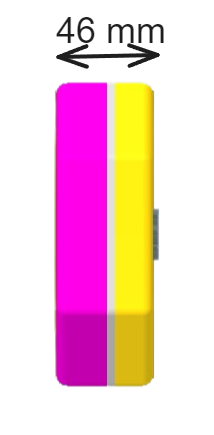
\includegraphics[height=4 cm]{texs/Part1/chapter4/image/v23.png}
        \end{minipage}
        \caption{Right View}
        \label{fig:variant2_right_view}
    \end{subfigure}
    \caption{Views of Preliminary Design Variant 2}
    \label{fig:variant2_views}
\end{figure}

\begin{figure}[h!]
    \centering
    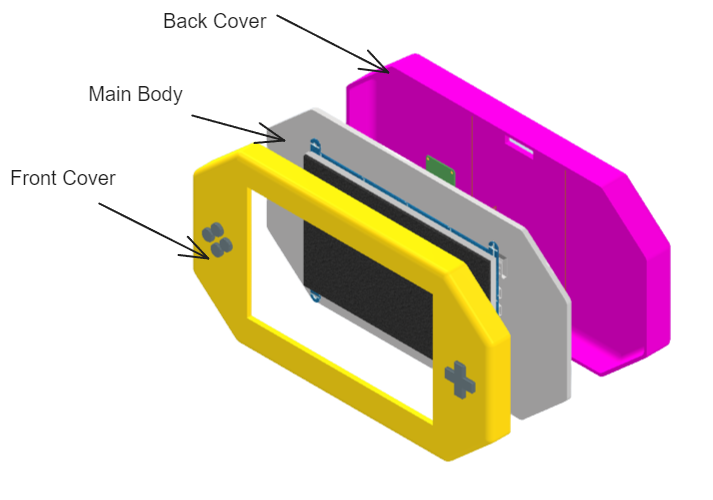
\includegraphics[width=0.5\linewidth]{texs/Part1/chapter4/image/v24.png}
    \caption{Body Components of Preliminary Design Variant 2}
    \label{fig:variant2_body_components}
\end{figure}

\begin{figure}[h!]
    \centering
    \begin{subfigure}[c]{0.5\textwidth}
        \begin{minipage}{\textwidth}
            \centering
            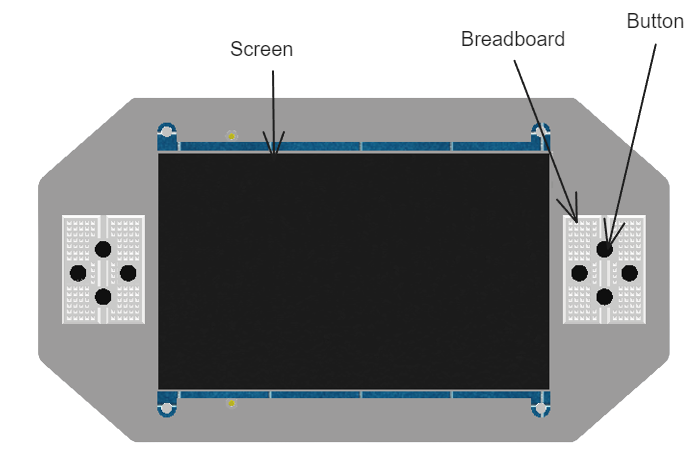
\includegraphics[height=4 cm]{texs/Part1/chapter4/image/v25.png}
        \end{minipage}
        \caption{Front View}
        \label{fig:variant2_front_view_main}
    \end{subfigure}
    % \hfill
    \begin{subfigure}[c]{0.5\textwidth}
        \begin{minipage}{\textwidth}
            \centering
            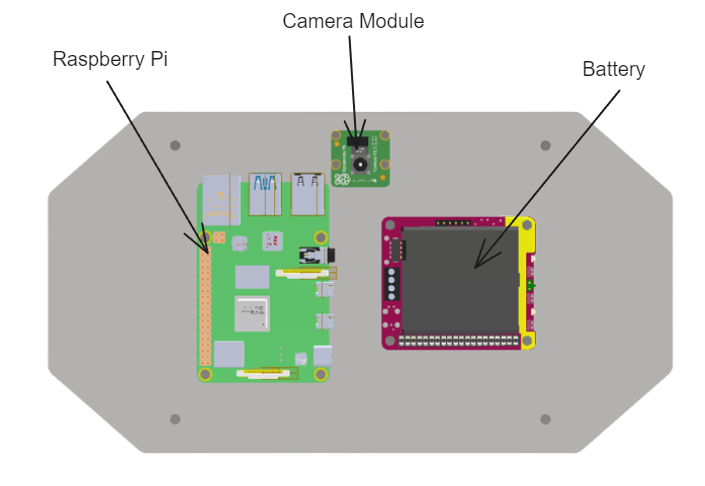
\includegraphics[height=4 cm]{texs/Part1/chapter4/image/v26.png}
        \end{minipage}
        \caption{Back View}
        \label{fig:variant2_back_view_main}
    \end{subfigure}
    \caption{Placement of inner components for Variant 2}
    \label{fig:variant2_inner_components}
\end{figure}

The physical design of Solution Variant 2 adheres to a sandwich-like structure comprising a main body, top cover, and back cover (Figure \ref{fig:variant2_body_components}). This design choice not only ensures the protection of internal components, but also simplifies assembly and maintenance. The main body of the device functions as the central hub, accommodating the internal components and features, whereas the top and back covers act as protective shields, safeguarding the internal parts from any damage that may result from external factors.

A crucial aspect of the design involves the arrangement of internal components within the device. Following a tablet-like configuration, the main LCD is positioned on the front side of the main body, providing users with a clear and interactive interface (Figure \ref{fig:variant2_front_view_main}). Simultaneously, the camera, Raspberry Pi, and battery were strategically placed on the back side of the body (Figure \ref{fig:variant2_back_view_main}) to optimize the weight distribution and ensure a well-balanced user experience. This arrangement enhances the overall usability and convenience of the device, making it suitable for a wide range of applications.

\begin{figure}[ht!]
    \centering
    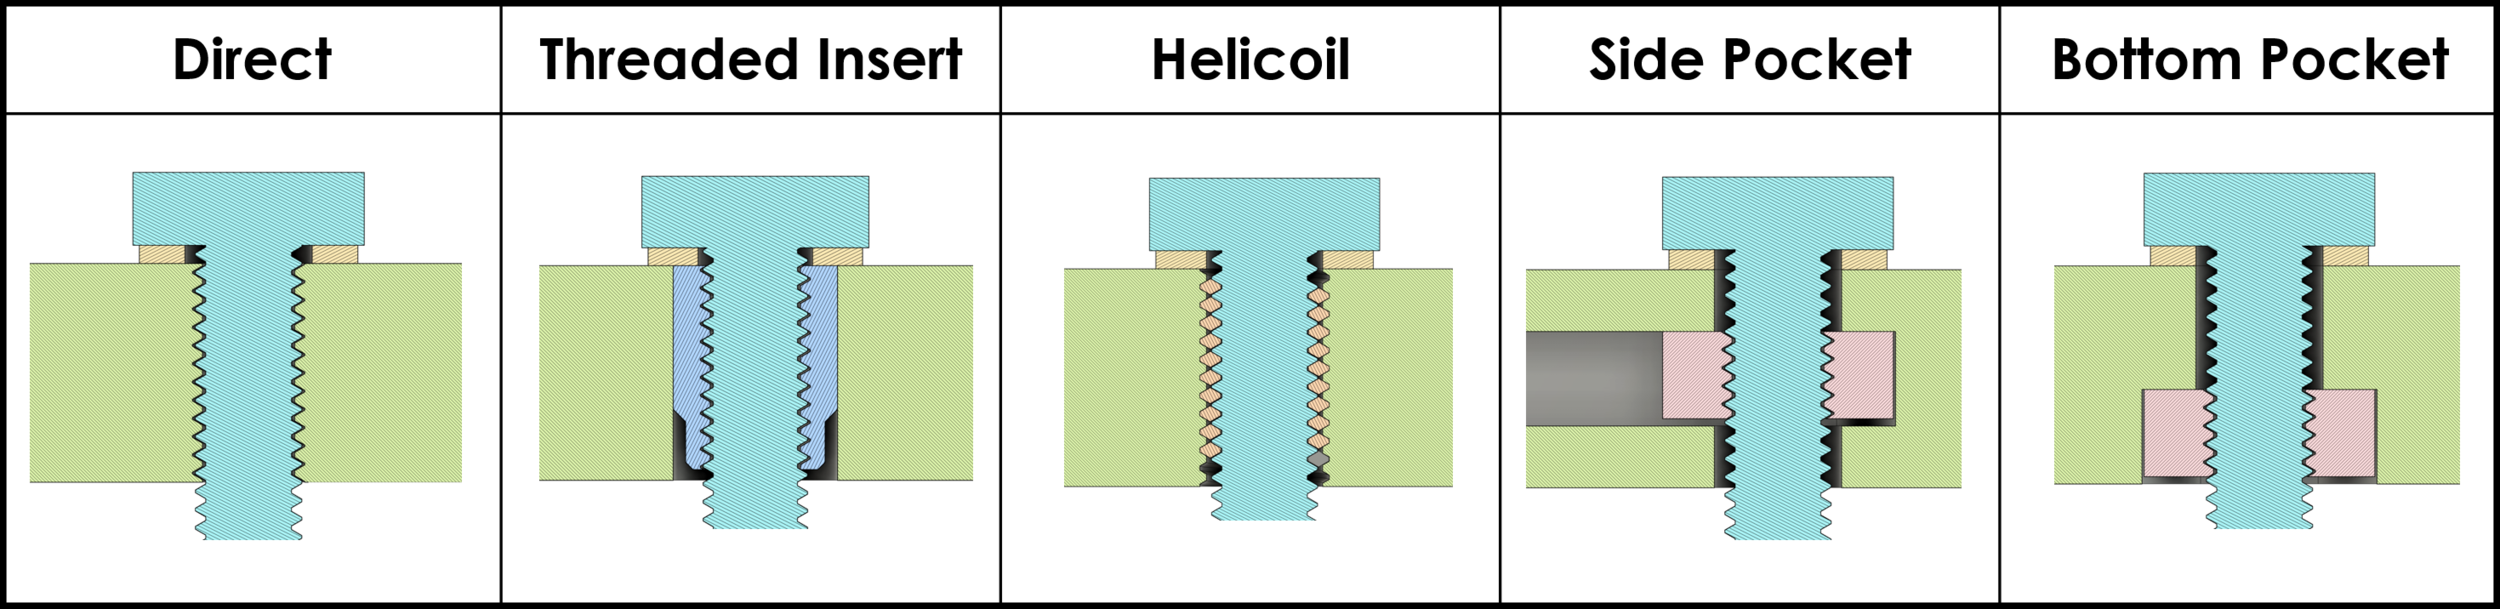
\includegraphics[width=\linewidth]{texs/Part1/chapter4/image/insert.png}
    \caption{Methods to secure components \cite{Hermann20}}
    \label{fig:insert}
\end{figure}

Ensuring the secure attachment of internal components to the main body is of primary importance in the design process. Various methods of component fastening have been considered, including direct attachment, threaded inserts, helicoils, side pockets, and bottom pockets, as shown in Figure \ref{fig:insert}.

The simplest approach is direct attachment, in which threads are designed into a 3D printed part to allow components to be screwed in. For more robust connections, threaded inserts can be used by designing holes in the 3D printed part and installing inserts appropriately.

Helicoils offer durable threaded holes by inserting coil-shaped inserts into the holes. Side pockets and bottom pockets involve creating cavities or slots in the 3D printed part to hold components securely. Each method has its own advantages and challenges. After careful evaluation, the variant opts for the use of threaded inserts due to its simplicity and robustness.

The battery, which is a critical component of the device, requires special attention to prevent any undesirable movement or instability. To address this concern, an effective method for firmly securing the battery in place is implemented by utilizing a battery cover. Figure \ref{fig:variant2_battery_cover} illustrates the design of the battery cover. The battery cover is then securely attached using screws and standoffs, ensuring that the battery remains in its designated position, even during vigorous handling or movement. Figure \ref{fig:variant2_battery_placement} shows the method used to secure the battery to the main body.

\begin{figure}[h!]
    \centering
    \begin{subfigure}[c]{\textwidth}
        \begin{minipage}{\textwidth}
            \centering
            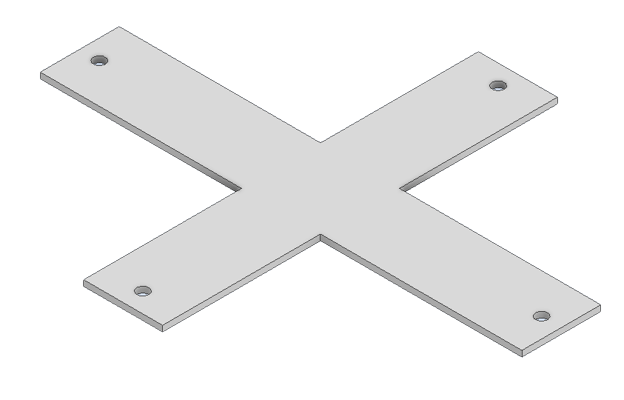
\includegraphics[height=4 cm]{texs/Part1/chapter4/image/v27.png}
        \end{minipage}
        \caption{Battery Cover}
        \label{fig:variant2_battery_cover}
    \end{subfigure}
    % \hfill
    \begin{subfigure}[c]{\textwidth}
        \begin{minipage}{\textwidth}
            \centering
            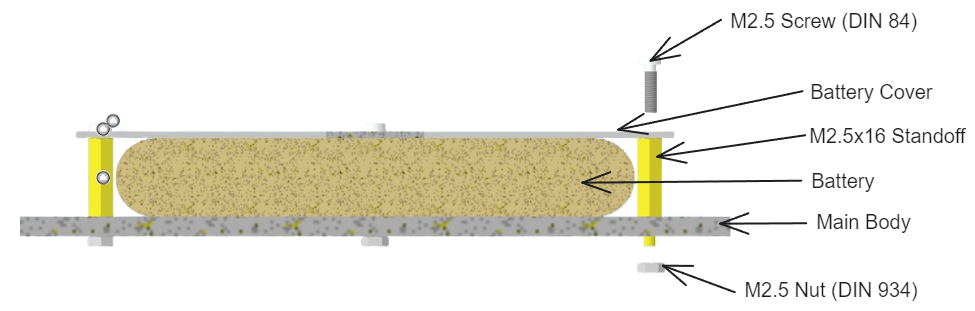
\includegraphics[height=3 cm]{texs/Part1/chapter4/image/v28.png}
        \end{minipage}
        \caption{Placement of components}
        \label{fig:variant2_battery_placement}
    \end{subfigure}
    \caption{Methods to secure the battery}
    \label{fig:variant2_battery}
\end{figure}

Solution Variant 2 employs a hybrid input method that combines both touch screen and physical buttons. The touch screen is oriented in landscape mode, while the buttons are positioned on either side of the screen (Figure \ref{fig:variant2_front_view}). To enable the integration of the touch screen, HDMI and USB connections were established between the touch screen and Raspberry Pi. Additionally, to facilitate the functionality of the physical buttons, they are connected to Raspberry Pi using general-purpose input/output  (GPIO) pins.

\begin{figure}[ht!]
    \centering
    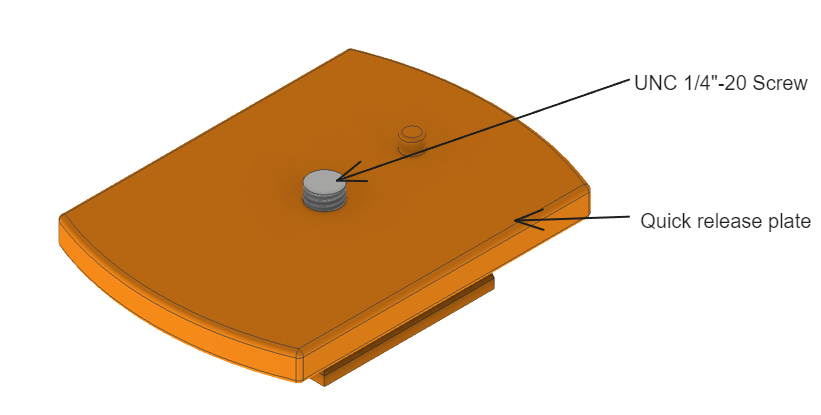
\includegraphics[height=5 cm]{texs/Part1/chapter4/image/v29.png}
    \caption{Quick release plate}
    \label{fig:variant2_quick_release_plate}
\end{figure}

In Figure \ref{fig:variant2_quick_release_plate}, we observe a quick release plate designed to be affixed to the tripod stand. To enhance stability during usage, Solution Variant 2 can utilize a quick release plate, which can be conveniently mounted on a tripod stand.

\subsubsection{Cost Calculation}
In this section, we will perform a cost analysis for producing Solution Variant 2. It is essential to emphasize that the cost calculation for the 3D printed parts solely considers the material cost and the estimated energy consumption during the printing process. Other expenses, such as the cost of the 3D printer itself, labor, and maintenance, are not factored into the calculation. Additionally, for better comparability with other variants, the costs of the Raspberry Pi, camera module, touch screen, and battery will not be included in the calculation. The formula used to calculate the cost of the 3D printed parts is as follows:

\dots


\subsection{Preliminary Design Variant 3}
\label{subsec:preliminary_design_variant_3}
Variant 3 maintains a similar component arrangement to variant 2, with the screen at the front and the camera, Raspberry Pi, and battery at the rear, as shown in Figure \ref{fig:variant3_inner_components}. However, Variant 3 introduced significant changes, such as a portrait-oriented screen and battery type.

\begin{figure}[h!]
    \centering
    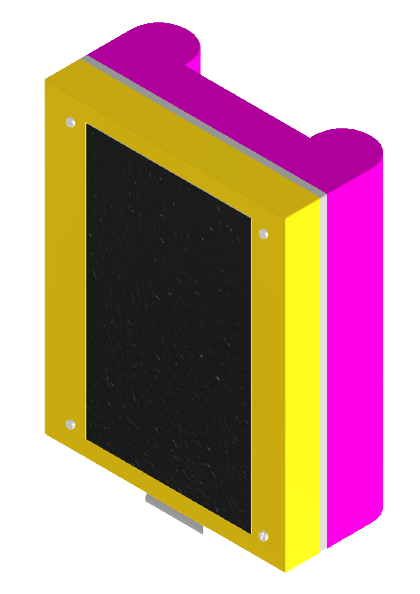
\includegraphics[height=5 cm]{texs/Part1/chapter4/image/v31.png}
    \caption{Preliminary Design Variant 3}
    \label{fig:preliminary_design_variant_3}
\end{figure}

\begin{figure}[h!]
    \centering
    \begin{subfigure}[c]{0.47\textwidth}
        \begin{minipage}{\textwidth}
            \centering
            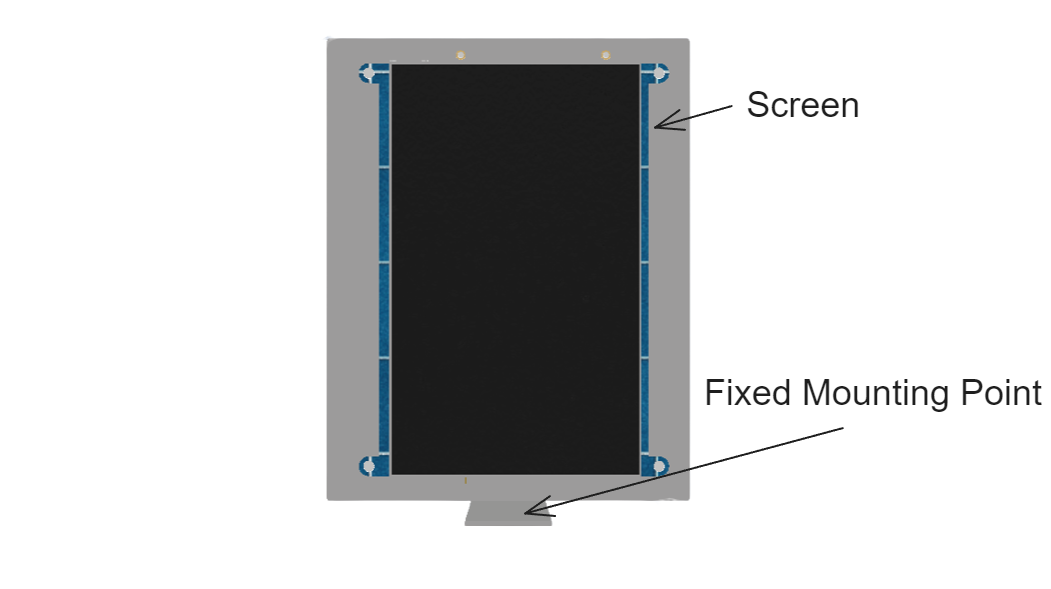
\includegraphics[height=4 cm]{texs/Part1/chapter4/image/v32.png}
        \end{minipage}
        \caption{Front View}
        \label{fig:variant3_front_components}
    \end{subfigure}
    % \hfill
    \begin{subfigure}[c]{0.5\textwidth}
        \begin{minipage}{\textwidth}
            \centering
            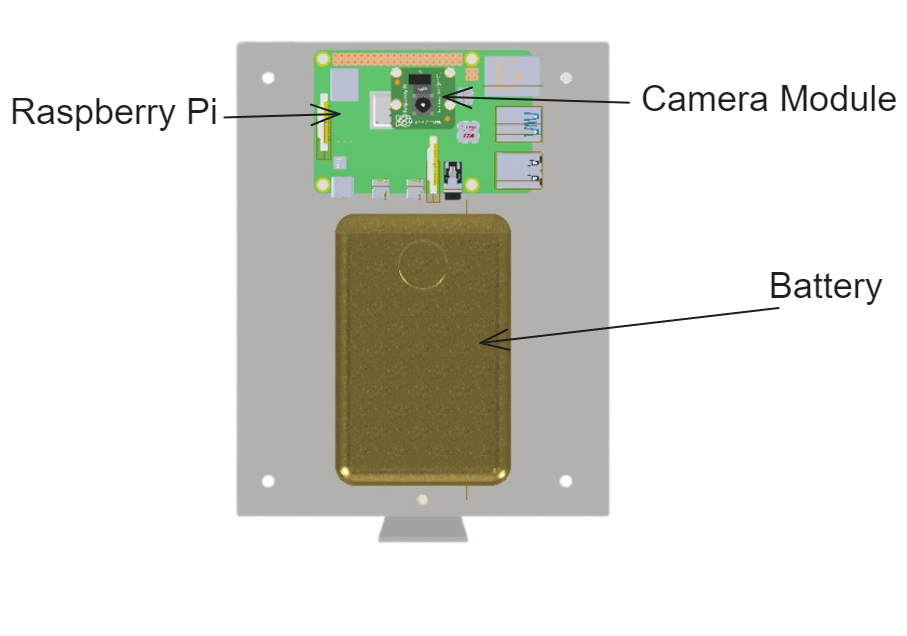
\includegraphics[height=4 cm]{texs/Part1/chapter4/image/v33.png}
        \end{minipage}
        \caption{Back View}
        \label{fig:variant3_back_components}
    \end{subfigure}
    \caption{Placement of inner components for Variant 3}
    \label{fig:variant3_inner_components}
\end{figure}

The chassis structure, similar to variant 2, comprises a main body, top cover, and back cover. The main body accommodates essential electronics and functional elements, while the top and back covers protect the internal components from external forces.

A noteworthy alteration is the inclusion of bumps on the back cover to enhance the ergonomics (Figure \ref{fig:variant3_bumps}). This adjustment aims to provide a more comfortable grip, improve user engagement, and extend the usability. In addition, the tactile bump serves as a subtle yet impactful refinement, ensuring that the device fits snugly in the user's hand, further enhancing the overall user experience. This thoughtful design element contributes to seamless and enjoyable interaction with the device.

\begin{figure}[h!]
    \centering
    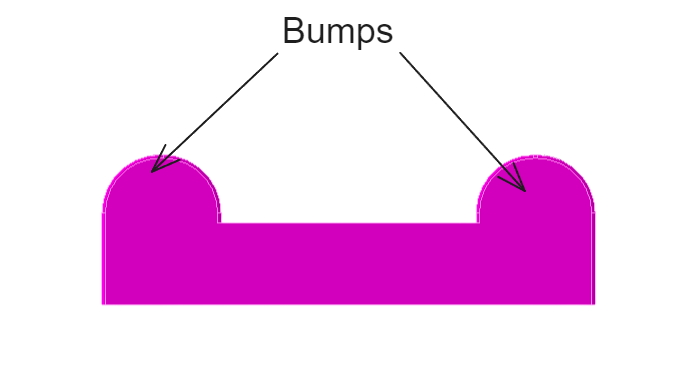
\includegraphics[width=0.5\linewidth]{texs/Part1/chapter4/image/v34.png}
    \caption{Bumps on the back cover}
    \label{fig:variant3_bumps}
\end{figure}

Variant 3 diverted from the standard battery position seen in variant 2, with a more noticeable difference in battery placement. Figure \ref{fig:variant3_battery_placement} illustrates a designated slot within the back cover, strategically designed to house a power bank outside the chassis. This configuration not only enhances the operational stability but also simplifies the process of battery replacement.

\begin{figure}[h!]
    \centering
    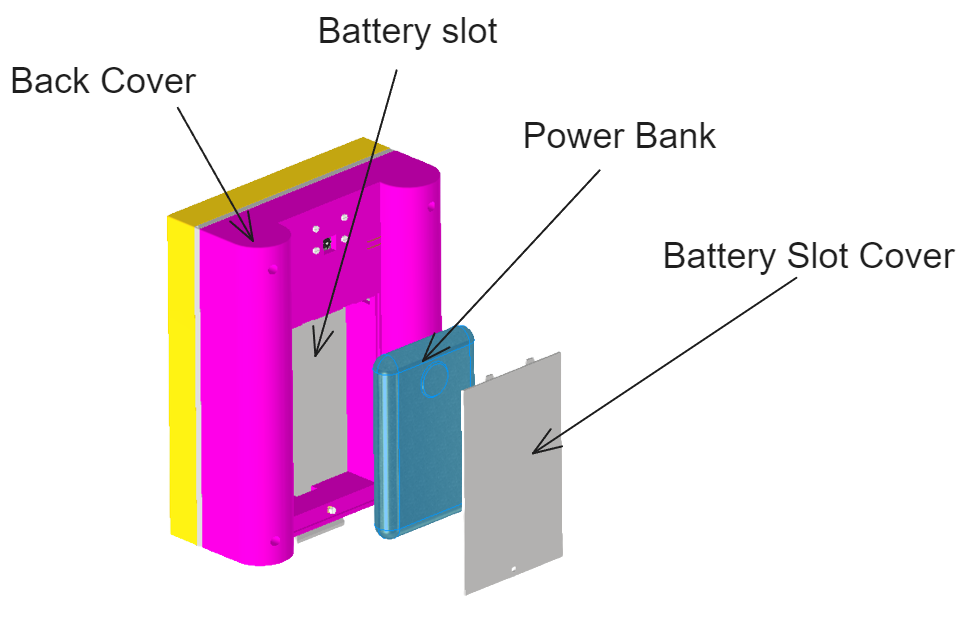
\includegraphics[width=0.5\linewidth]{texs/Part1/chapter4/image/v35.png}
    \caption{Battery Placement}
    \label{fig:variant3_battery_placement}
\end{figure}

The input methodology was streamlined using a touch screen as the sole interface. This approach simplifies the user experience by eliminating the need for physical buttons and by seamlessly integrating screen interactions. Additional information regarding the integration of the touchscreen with the Raspberry Pi is provided in the previous section.

Figure \ref{fig:variant3_front_components} also shows the integration of the mounting point of the tripod directly with the main body in Variant 3. This strategic design allows the mounting point to serve as a sturdy anchor for the device when used in a tripod stand. This direct union ensures secure and stable attachment, enhancing the versatility of the device across various usage scenarios.

\subsubsection{Cost Calculation}

\subsection{Preliminary Design Variant 6}
\label{subsec:preliminary_design_variant_6}
Figure \ref{fig:preliminary_design_variant_6} provides a detailed and comprehensive overview of the initial design concept of Variant 6. This version stands out by organizing its internal components into a configuration resembling a point-of-service (POS) system. This change from previous iterations purposefully positions the screen at an inclined angle, enhancing user interaction and optimizing the screen visibility (Figure \ref{fig:variant6_inner_components}).

\begin{figure}[h!]
    \centering
    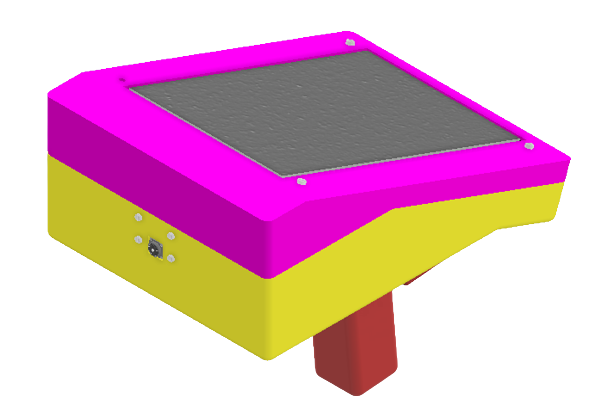
\includegraphics[height=5 cm]{texs/Part1/chapter4/image/v61.png}
    \caption{Preliminary Design Variant 6}
    \label{fig:preliminary_design_variant_6}
\end{figure}

\begin{figure}[h!]
    \centering
    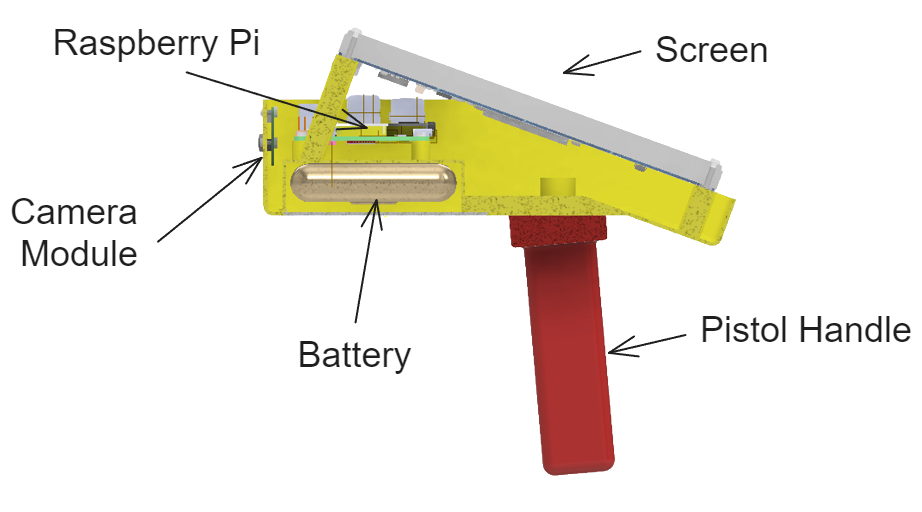
\includegraphics[height=5 cm]{texs/Part1/chapter4/image/v62.png}
    \caption{Placement of inner components for Variant 3}
    \label{fig:variant6_inner_components}
\end{figure}


Figure \ref{fig:variant6_handle_grip} demonstrates the design of the handle grip, while Figure \ref{fig:variant6_handle_grip_main_body} illustrates its placement on the main body. This ergonomic addition ensures a secure and comfortable hold during operation. Additionally, the handling of the device can be easily switched between the quick-change plate and the handle grip, providing users with flexible options for different scenarios (see Figure \ref{fig:variant6_quick_release_plate_main_body}).

\begin{figure}[h!]
    \centering
    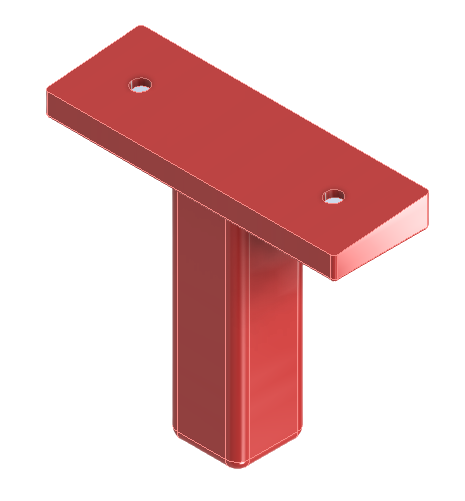
\includegraphics[width=0.5\linewidth]{texs/Part1/chapter4/image/v65.png}
    \caption{Handle Grip}
    \label{fig:variant6_handle_grip}
\end{figure}

\begin{figure}[h!]
    \centering
    \begin{subfigure}[c]{0.47\textwidth}
        \begin{minipage}{\textwidth}
            \centering
            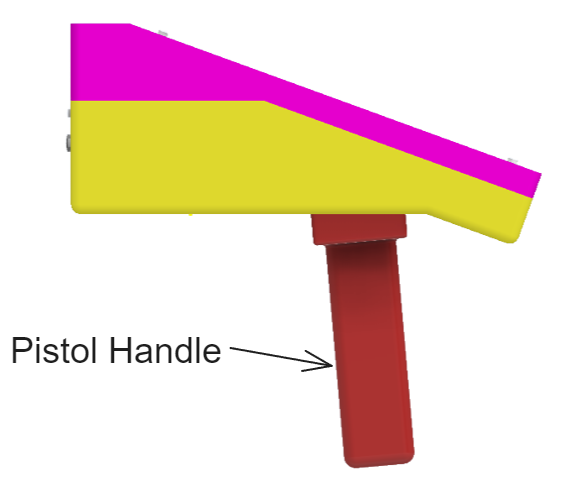
\includegraphics[height=4 cm]{texs/Part1/chapter4/image/v63.png}
        \end{minipage}
        \caption{Handle Grip with Main Body}
        \label{fig:variant6_handle_grip_main_body}
    \end{subfigure}
    % \hfill
    \begin{subfigure}[c]{0.5\textwidth}
        \begin{minipage}{\textwidth}
            \centering
            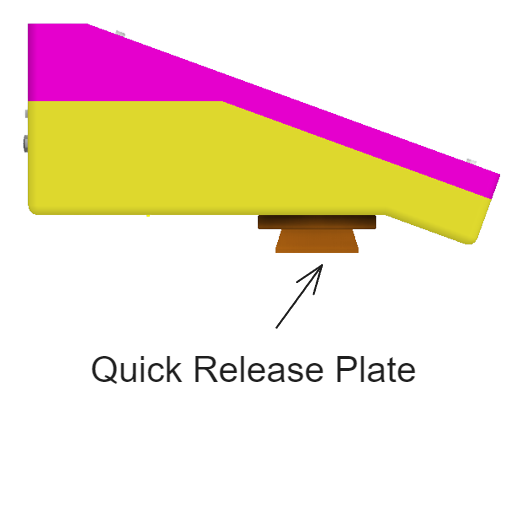
\includegraphics[height=4 cm]{texs/Part1/chapter4/image/v64.png}
        \end{minipage}
        \caption{Quick Release Plate with Main Body}
        \label{fig:variant6_quick_release_plate_main_body}
    \end{subfigure}
    \caption{Placement of handle grip and quick release plate}
    \label{fig:variant6_handle_grip_quick_release_plate}
\end{figure}


This variant boasts the same input method and battery placement as Variant 3. For a comprehensive explanation regarding these aspects, please refer to Section \ref{subsec:preliminary_design_variant_3}. Touch screens serve as the primary input modality, providing an intuitive and seamless interaction experience. Furthermore, the battery is tucked away in a slot on the back cover and is secured by screws and threaded inserts.

\subsubsection{Cost Calculation}


\subsection{Preliminary Design Variant 7}
Figure \ref{fig:preliminary_design_variant_7} shows the intriguing concept of variant 7, which is influenced by the handheld PC approach. Here, Raspberry Pi cleverly integrates with the back of the screen, forming a compact and unified structure. Simultaneously, the battery aligned gracefully beside the screen, creating a harmonious arrangement.

\begin{figure}[h!]
    \centering
    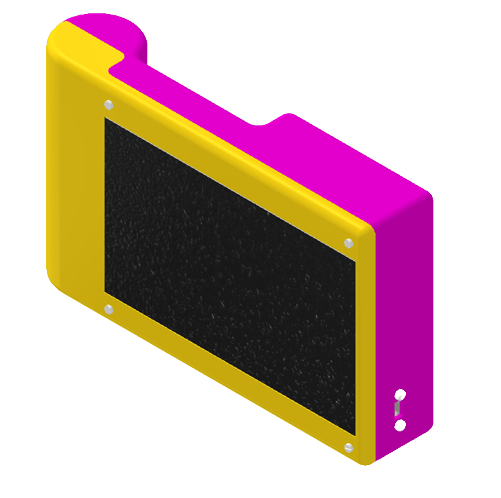
\includegraphics[height=5 cm]{texs/Part1/chapter4/image/v71.png}
    \caption{Preliminary Design Variant 7}
    \label{fig:preliminary_design_variant_7}
\end{figure}

\begin{figure}[h!]
    \centering
    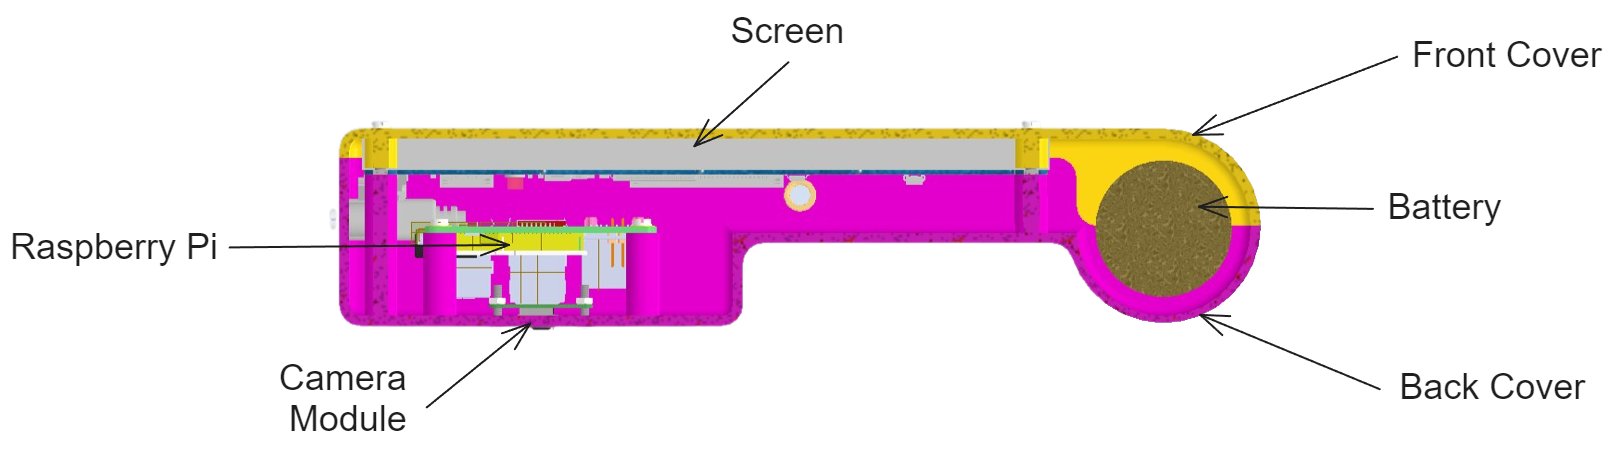
\includegraphics[height=3 cm]{texs/Part1/chapter4/image/v72.png}
    \caption{Placement of inner components for Variant 7}
    \label{fig:variant7_inner_components}
\end{figure}

The device features a strategically placed bump on the side, which improves ergonomics and serves as a secure enclosure for the battery (Figure \ref{fig:variant7_inner_components}). The control methods in this variant were similar to those in variant 2, utilizing only touch interfaces.

\begin{figure}[h!]
    \centering
    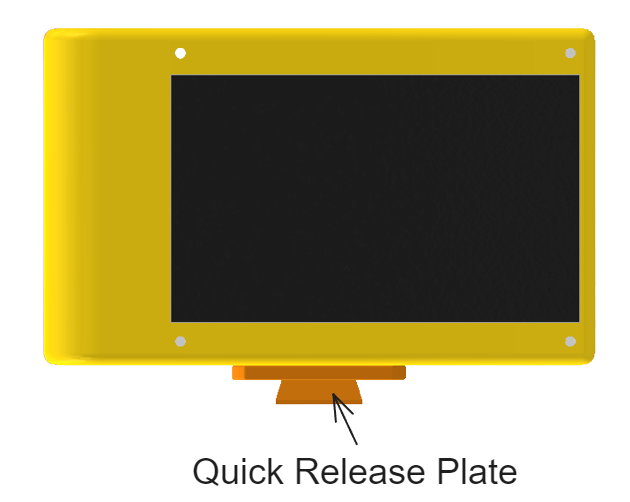
\includegraphics[height=5 cm]{texs/Part1/chapter4/image/v73.png}
    \caption{Placement of quick release plate}
    \label{fig:variant7_quick_release_plate}
\end{figure}

Similar to variants 2 and 6, this variant also utilized the quick release plate to enable integration with a tripod stand. The placement of the plate can be seen in Figure \ref{fig:variant7_quick_release_plate}.



\subsubsection{Cost Calculation}

\section{Evaluation of Preliminary Design Variants}
VDI 2225

\subsection{Evaluation Criteria}

The technical evaluation criteria are primarily derived from the list of requirements but can also be established from general conditions. The property dimensions can be captured through specific metrics as well as qualitative statements. When establishing the evaluation criteria, it must be noted that the individual goals to be evaluated are largely independent from each other. The identified criteria must be formulated positively, as this enables better alignment with the corresponding value concepts.37 The following evaluation criteria are used for the technical assessment of the various variants:

\textbf{Ergonomics:} The ergonomics of the variants are evaluated based on the following criteria: \textit{handling, weight, and dimensions}. The handling is assessed based on the ease of use and the intuitive operation of the variants. The weight is evaluated based on the weight of the variants and the weight distribution. The dimensions are assessed based on the size of the variants and the size of the individual components.

\textbf{Weight Distribution:} The weight distribution is evaluated based on the weight distribution of the variants and the weight distribution of the individual components. The value for weight distribution is retrieved from Computer-Aided Design (CAD) models through detailed analysis of the device's structural layout and component placement.

\textbf{Device Weight:} Device weight evaluates the overall heaviness of the equipment. A lighter device is generally easier to handle and transport, reducing user fatigue and enabling greater mobility while maintaining performance and durability. The value for device weight is calculated from Computer-Aided Design (CAD) models by summing the individual weights of all components, materials, and structural elements that constitute the device.

\textbf{Device Size:} The size criterion considers the physical dimensions of the device, assessing its compactness and portability. An optimal device size allows for convenient storage, transportation, and operation in various environments without compromising functionality. The evaluation of device size involves measuring key dimensions such as length, width, height, and any protrusions or extensions.

\textbf{Ease of Assembly:} This criterion focuses on the simplicity and efficiency of assembling and disassembling the device. A design that enables quick and hassle-free assembly and disassembly not only saves time but also enhances user convenience and reduces the risk of errors. Evaluation is conducted by assessing the number of components involved in the assembly and disassembly processes. A lower count of components often indicates a simpler and more user-friendly design. Additionally, the type and quantity of fasteners, such as screws or connectors, required for assembly are taken into account. A reduced reliance on intricate fastening mechanisms contributes to smoother handling and maintenance. By quantifying these factors, designers can gauge the ease of assembly and disassembly, enabling them to refine the design to optimize user-friendliness and operational efficiency.

\textbf{Swappable Parts:} Swappable parts assess the ease with which components or parts of the device can be interchanged or replaced. A design that facilitates swappable parts enhances flexibility, maintenance, and adaptability to different tasks or conditions. Swappable parts promote component modularity, enabling efficient repairs and upgrades. The evaluation of swappable parts is based on the number of interchangeable components and their compatibility across the device. A higher number of swappable parts indicates a design that encourages versatility and minimizes downtime during maintenance or repairs. This modularity simplifies troubleshooting and allows users to adapt the device to evolving needs or specialized requirements. By quantifying the availability of swappable parts, designers can ensure a design that empowers users to swiftly and effectively manage the device's functionality, enhancing its overall usability and lifespan.

\textbf{Durability to External Factors:} Durability to external factors evaluates how well the device can withstand exposure to various environmental conditions, such as humidity, temperature fluctuations, dust, and impacts. A high level of durability ensures a longer lifespan and consistent performance under diverse circumstances. The assessment of durability is measured by estimating the number of openings in the device. More openings can lead to greater exposure of inner components, potentially making them susceptible to external elements. Therefore, a design with fewer openings is considered more resilient, as it reduces the likelihood of environmental factors affecting critical components. By quantifying the number of openings and assessing their placement, designers can enhance the device's ability to endure harsh conditions and maintain reliable functionality over time, ultimately extending its operational life and user satisfaction.




\chapter{Printing and Assembly}
\label{ch:printingandassembly}

\section{Printing}
\label{sec:printing}

In this section, we will describe the printing process for the prototype. This process was carried out at the Workshop of the University of Applied Sciences Brandenburg using the printer described in Section \ref{subsec:prusa_slicer_mk3s}. The following parameters are utilized for the process.

\begin{itemize}
    \item Layer Height: 0.2 mm
    \item Infill Density: 15 \%
    \item Print Speed: 60 mm/s
    \item Supports: Everywhere
    \item Filament: PLA
\end{itemize}

Table \ref{tab:finalprintingtimeandfilament} provides information on the printing time and the weight of filament used. Additionally, Figure \ref{fig:printedparts} showcases the final printed parts after removing the support materials.


\begin{table}[!ht]
    \centering
    \begin{tabular}{|l|c|c|}
        \hline
        \textbf{Part Name} & \textbf{Weight of PLA used (g)} & \textbf{Printing Time (h)} \\ \hline
        Top Cover          & 57.71                           & 2.00                       \\ \hline
        Main Body          & 245.14                          & 9.25                       \\ \hline
        Battery Cover      & 22.21                           & 0.67                       \\ \hline
        Switch Cover       & 1.31                            & 0.05                       \\ \hline
        Handle Pistol      & 64.63                           & 1.98                       \\ \hline
    \end{tabular}
    \caption{Printing Time and Filament Used}
    \label{tab:finalprintingtimeandfilament}
\end{table}

\begin{figure}[!ht]
    \centering
    \begin{subfigure}[c]{0.45\textwidth}
        \begin{minipage}{\textwidth}
            \centering
            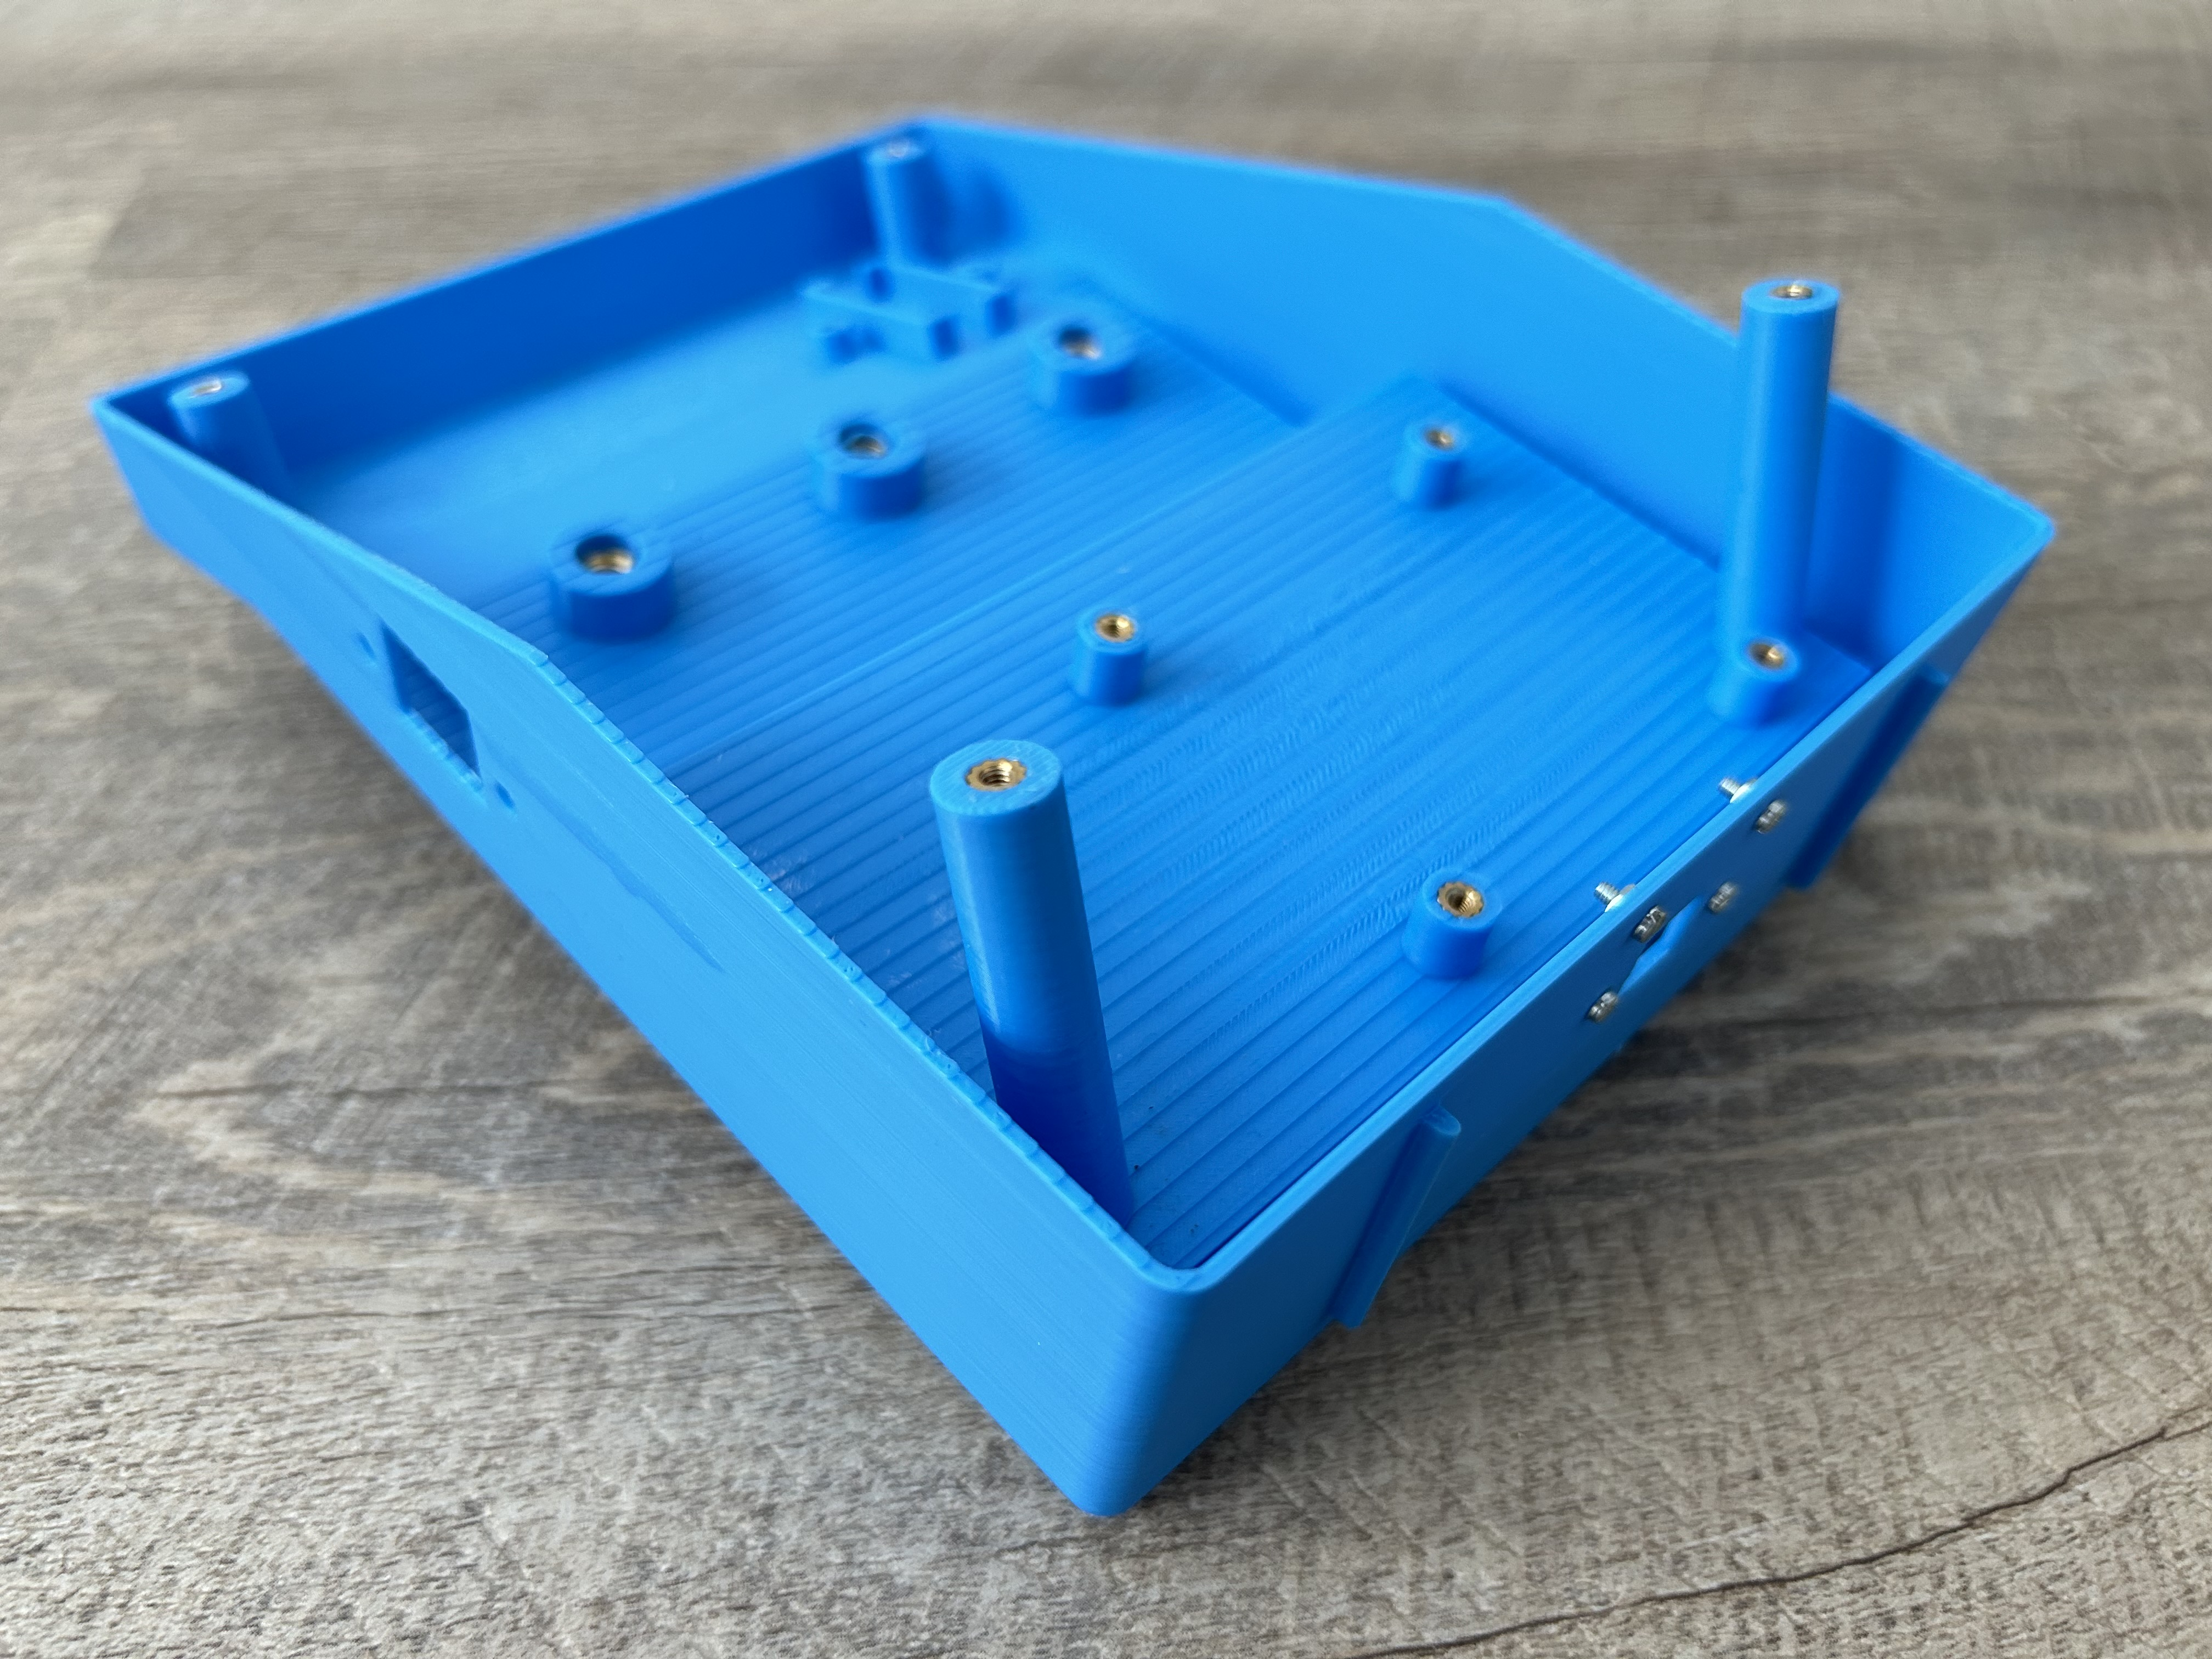
\includegraphics[height=4 cm]{texs/Part1/chapter5/image/res_main.jpg}
        \end{minipage}
        \caption{Main Body}
        \label{fig:printed_main_body}
    \end{subfigure}
    \begin{subfigure}[c]{0.45\textwidth}
        \begin{minipage}{\textwidth}
            \centering
            \includegraphics[height=4 cm]{texs/Part1/chapter5/image/res_top.jpg}
        \end{minipage}
        \caption{Top Cover}
        \label{fig:printed_top_cover}
    \end{subfigure}
    \begin{subfigure}[c]{0.45\textwidth}
        \begin{minipage}{\textwidth}
            \centering
            \includegraphics[height=4 cm]{texs/Part1/chapter5/image/res_batt.jpg}
        \end{minipage}
        \caption{Battery Cover}
        \label{fig:printed_battery_cover}
    \end{subfigure}
    \begin{subfigure}[c]{0.45\textwidth}
        \begin{minipage}{\textwidth}
            \centering
            \includegraphics[height=4 cm]{texs/Part1/chapter5/image/res_switch.jpg}
        \end{minipage}
        \caption{Switch Cover}
        \label{fig:printed_switch_cover}
    \end{subfigure}
    \begin{subfigure}[c]{0.45\textwidth}
        \begin{minipage}{\textwidth}
            \centering
            \includegraphics[height=4 cm]{texs/Part1/chapter5/image/res_grip.jpg}
        \end{minipage}
        \caption{Handle Pistol}
        \label{fig:printed_handle_pistol}
    \end{subfigure}
    \caption{Printed Parts}
    \label{fig:printedparts}
\end{figure}

\section{Assembly}
\label{sec:assembly}

The assembly process is done by following the steps below:

\subsubsection{Step 1: Installation of Threaded Inserts}
In order to securely install the brass threaded inserts into the main body, it is recommended to use a soldering iron \cite{Hermann23}. Begin by placing the chosen threaded insert onto the targeted position, aligning it with the desired hole. Heat the soldering iron to a suitable temperature, ranging from 225 $^{\circ}C$ to 245 $^{\circ}C$ for PLA material.

Once the soldering iron has reached the appropriate temperature, apply it gently to the top of the threaded insert. This process will transmit controlled heat into the material, causing the wall to soften and allow the threaded insert to be inserted. For a visual representation of how a threaded insert should look once correctly installed into the main body, please refer to Figure \ref{fig:threadedinsert}.

\begin{figure}[!ht]
    \centering
    \includegraphics[height=5cm]{texs/Part1/chapter5/image/threadinstall.jpg}
    \caption{The installed threaded insert}
    \label{fig:threadedinsert}
\end{figure}

\subsubsection{Step 2: Installation of Switch}
Installing a switch to the main body is a straightforward process that requires a few basic materials: the switch itself, a switch cover, two M2.5 nuts, and M2.5 screws. Position the switch inside the designated switch holder (see Figure \ref{fig:switchholder}), ensuring that the button faces outward for easy access.

Next, the switch cover is placed on top, aligning it with the switch and the corresponding holes in the main body. Once aligned, the M2.5 screws and nuts secure the switch and the cover to the main body. Figure \ref{fig:switchinstall} shows the completed installation of the switch.

\begin{figure}[!ht]
    \centering
    \includegraphics[height=5cm]{texs/Part1/chapter5/image/switchhole.png}
    \caption{The Switch Holder}
    \label{fig:switchholder}
\end{figure}

\begin{figure}[!ht]
    \centering
    \includegraphics[height=5cm]{texs/Part1/chapter5/image/switchinstall.jpg}
    \caption{The installed switch}
    \label{fig:switchinstall}
\end{figure}

\subsubsection{Step 3: Installation of LAN Port}

This step begins by locating the slot of the LAN port on the main body, which is located on the right side of the main body (see Figure \ref{fig:lanslot}). The LAN port is inserted into the slot and secured using the M3 screws. Figure \ref{fig:laninstall} shows the completed installation of the LAN port.

\begin{figure}[!ht]
    \centering
    \includegraphics[height=5cm]{texs/Part1/chapter5/image/lanslot.png}
    \caption{The LAN Port Slot}
    \label{fig:lanslot}
\end{figure}

\begin{figure}[!ht]
    \centering
    \includegraphics[height=5cm]{texs/Part1/chapter5/image/laninstall.jpg}
    \caption{The installed LAN port}
    \label{fig:laninstall}
\end{figure}

\subsubsection{Step 4: Installation of Camera Module}

The camera module is installed to the main body using M2 screws. The camera module is placed in the designated slot on the main body (see Figure \ref{fig:cameraslot}). The M2 screws are then used to secure the camera module to the main body. Figure \ref{fig:camerainstall} shows the completed installation of the camera module.

\begin{figure}[!ht]
    \centering
    \includegraphics[height=5cm]{texs/Part1/chapter5/image/camslot.png}
    \caption{The Camera Module Slot}
    \label{fig:cameraslot}
\end{figure}

\begin{figure}[!ht]
    \centering
    \includegraphics[height=5cm]{texs/Part1/chapter5/image/caminstall.jpg}
    \caption{The installed camera module}
    \label{fig:camerainstall}
\end{figure}

\subsubsection{Step 5: Installation of Battery}
To start the installation process, insert the battery into the holder as shown in Figure \ref{fig:batteryholder}. Then, connect the battery to the switch with a 90-degree USB-A to USB-C connector.

To fasten the battery to the main body, place the battery cover over the battery and main body. Use the M2.5 screws to secure the battery cover to the main body. The finished battery installation can be seen in Figure \ref{fig:batteryinstall}.

\begin{figure}[!ht]
    \centering
    \includegraphics[height=5cm]{texs/Part1/chapter5/image/battslot.png}
    \caption{The Battery Holder}
    \label{fig:batteryholder}
\end{figure}

\begin{figure}[ht!]
    \centering
    \begin{subfigure}[c]{0.45\textwidth}
        \begin{minipage}{\textwidth}
            \centering
            \includegraphics[height=5 cm]{texs/Part1/chapter5/image/battinstall1.jpg}
        \end{minipage}
        \caption{Without Battery Cover}
        \label{fig:battery_install_1}
    \end{subfigure}
    \begin{subfigure}[c]{0.45\textwidth}
        \begin{minipage}{\textwidth}
            \centering
            \includegraphics[height=5 cm]{texs/Part1/chapter5/image/battinstall2.jpg}
        \end{minipage}
        \caption{With Battery Cover}
        \label{fig:battery_install_2}
    \end{subfigure}
    \caption{The installed battery}
    \label{fig:batteryinstall}
\end{figure}

\subsubsection{Step 6: Installation of Raspberry Pi}

The Raspberry Pi is installed on the main body by using the M2.5 screws. The Raspberry Pi is placed in the designated slot on the main body (see Figure \ref{fig:raspislot}). The M2.5 screws are then used to secure the Raspberry Pi to the main body.

Next, the following connections are made to the Raspberry Pi:

\begin{itemize}
    \item The LAN port is connected to the Raspberry Pi via a LAN cable.
    \item The camera module is connected to the Raspberry Pi via a ribbon cable.
    \item The switch is connected to the Raspberry Pi via a USB-C cable.
\end{itemize}

\begin{figure}[!ht]
    \centering
    \includegraphics[height=5cm]{texs/Part1/chapter5/image/raspislot.png}
    \caption{The Raspberry Pi Slot}
    \label{fig:raspislot}
\end{figure}

\subsubsection{Step 7: Installation of Screen and Top Cover}

The final step is to install the screen and the top cover. Begin by placing the screen into the designated slot on the main body (see Figure \ref{fig:screenslot}) and align the hole on the screen with the hole on the main body. Next, the top cover is placed on top of the main body. The M2.5 screws are then used to secure the top cover to the main body. Figure \ref{fig:screeninstall} shows the completed installation of the screen and the top cover.

\begin{figure}[!ht]
    \centering
    \includegraphics[height=5cm]{texs/Part1/chapter5/image/screenslot.png}
    \caption{The Screen Slot}
    \label{fig:screenslot}
\end{figure}

\begin{figure}[!ht]
    \centering
    \includegraphics[height=5cm]{texs/Part1/chapter5/image/screeninstall.jpg}
    \caption{The installed screen and top cover}
    \label{fig:screeninstall}
\end{figure}

\section{Final Product}
\label{sec:finalproduct}

Figure \ref{fig:finalproduct} shows the final product. The total cost of building the product including the cost of printing and all of the materials is shown in Table \ref{tab:totalprintingcost} and Table \ref{tab:totalmaterialcost} respectively.

\begin{figure}[ht!]
    \centering
    \begin{subfigure}[c]{0.45\textwidth}
        \begin{minipage}{\textwidth}
            \centering
            \includegraphics[height=6 cm]{texs/Part1/chapter5/image/final1.jpg}
        \end{minipage}
    \end{subfigure}
    \begin{subfigure}[c]{0.45\textwidth}
        \begin{minipage}{\textwidth}
            \centering
            \includegraphics[height=6 cm]{texs/Part1/chapter5/image/final2.jpg}
        \end{minipage}
    \end{subfigure}
    \par\bigskip
    \begin{subfigure}[c]{0.45\textwidth}
        \begin{minipage}{\textwidth}
            \centering
            \includegraphics[height=6 cm]{texs/Part1/chapter5/image/final3.jpg}
        \end{minipage}
    \end{subfigure}
    \caption{The Final Product}
    \label{fig:finalproduct}
\end{figure}

\begin{table}[!ht]
    \centering
    \begin{tabular}{|l|c|c|c|}
        \hline
        \textbf{Part Name} & \textbf{Material Cost} & \textbf{Energy Cost} & \textbf{Total Cost} \\ \hline
        Top Cover          & 1.73 €                 & 0.04 €               & 1.77 €              \\ \hline
        Main Body          & 7.35 €                 & 0.17 €               & 7.53 €              \\ \hline
        Battery Cover      & 0.67 €                 & 0.01 €               & 0.68 €              \\ \hline
        Switch Cover       & 0.04 €                 & 0.00 €               & 0.04 €              \\ \hline
        Handle Pistol      & 1.94 €                 & 0.04 €               & 1.98 €              \\ \hline
        \textbf{Total}     & \textbf{11.73 €}       & \textbf{0.26 €}      & \textbf{11.99 €}    \\ \hline
    \end{tabular}
    \caption{Total Printing Cost}
    \label{tab:totalprintingcost}
\end{table}

\begin{table}[!ht]
    \centering
    \begin{tabular}{|l|c|c|c|c|}
        \hline
        \textbf{Parts Name}          & \textbf{Amount} & \textbf{Price} & \textbf{Remarks} & \textbf{Total Price} \\ \hline
        Printing Cost                & 1               & 11.99 €        & Calculated       & 11.99 €              \\ \hline
        RaspberyPi 4B 2GB            & 1               & 35.00 €        & RaspberryPi      & 35.00 €              \\ \hline
        Camera Module v2             & 1               & 25.00 €        & RaspberryPi      & 25.00 €              \\ \hline
        Waveshare 7inch screen       & 1               & 53.99 €        & Waveshare        & 53.99 €              \\ \hline
        Veektomx Battery             & 1               & 25.99 €        & Amazon           & 25.99 €              \\ \hline
        Screw M2x10mm (DIN 84)       & 4               & 0.05 €         & Wuerth           & 0.20 €               \\ \hline
        Screw M2.5x10mm (DIN 84)     & 7               & 0.05 €         & Wuerth           & 0.35 €               \\ \hline
        Screw M2.5x18mm (DIN 84)     & 4               & 0.11 €         & Wuerth           & 0.44 €               \\ \hline
        Screw M3x10mm (DIN 84)       & 2               & 0.05 €         & Wuerth           & 0.10 €               \\ \hline
        Nut M2 (DIN 934)             & 4               & 0.04 €         & Wuerth           & 0.15 €               \\ \hline
        Nut M2.5 (DIN 934)           & 2               & 0.04 €         & Wuerth           & 0.07 €               \\ \hline
        Threaded Inserts M2.5        & 9               & 0.13 €         & Ruthex           & 1.16 €               \\ \hline
        Threaded Inserts 1/4"        & 3               & 0.50 €         & Ruthex           & 1.50 €               \\ \hline
        1/4" Camera Screw            & 2               & 1.40 €         & Amazon           & 2.80 €               \\ \hline
        LAN Port                     & 1               & 5.67 €         & Aliexpress       & 5.67 €               \\ \hline
        Switch Pi                    & 1               & 3.90 €         & Amazon           & 3.90 €               \\ \hline
        90-Degree USB-A to USB-C     & 1               & 2.75 €         & Amazon           & 2.75 €               \\ \hline
        90-Degree USB-A to micro USB & 1               & 5.99 €         & Amazon           & 5.99 €               \\ \hline
        90-Degree HDMI               & 1               & 2.12 €         & Aliexpress       & 2.12 €               \\ \hline
        \textbf{Total}               & ~               & ~              & ~                & \textbf{168.29 €}    \\ \hline
    \end{tabular}
    \caption{Total Material Cost}
    \label{tab:totalmaterialcost}
\end{table}


\chapter{Conclusion}
In summary, this research has developed and demonstrated a highly promising handheld device engineered to measure vehicle speed precisely. This prototype is a cost-effective alternative to the existing speed measurement tools, particularly the conventional speed pistol. By integrating cheap computational components, high-quality cameras, and the power of 3D printing, we propose an affordable, highly accurate, and reliable device.

The design process of the prototype was carried out based on VDI guideline 2221 and divided into four parts: task clarification, conceptual design, embodiment design, and detail design. The task clarification phase was conducted by identifying the problem, defining the requirements, and setting the specifications.

The conceptual design phase was carried out by defining function and function structure. The function structure was then used to generate working principles with the help of brainstorming and analysis of existing technical systems. The result of idea generation is presented inside Zwicky's morphological box. The working principles are then combined to form eight different working structures. After careful evaluation, only four were selected for further development.

In the embodiment design phase, the four working structures were developed further by defining their 3D model with Autodesk Inventor. With the help of the 3D model, the working structures were evaluated based on their physical properties, manufacturability, and ergonomics. The estimated cost of manufacturing each variant is also calculated and compared. The evaluation results show that variant 6 is the most suitable to be chosen as the final design.

The detailed design phase was carried out by developing the final design of the prototype based on the chosen variant. In this phase, the 3D model of the prototype was developed further by adding more details and components. The 3D model was then used to generate the technical drawing of the prototype.

The final design was then manufactured using 3D printing technology. The prototype was assembled and tested to ensure it worked as intended. The test result shows that the prototype can securely hold the inner components properly and protect them. In terms of ergonomics, the handling of the device seems stable and lightweight.

The prototype of the speed pistol has been developed at a remarkably low cost, totaling only 168.29 €. This cost is significantly lower, approximately 90\%, compared to the conventional speed pistol discussed in Chapter \ref{chap:stateoftheart}. However, it is essential to note that this prototype cost does not serve as a direct indicator for setting the product's final selling price. Further development work is required to enhance the prototype's durability and reliability.

In other words, while the current prototype shows promise in terms of cost-efficiency, additional investment and refinement are necessary to ensure that the final product meets the necessary quality and performance standards, which may involve additional testing, material improvements, and refining the production process to create a market-ready product.

A proper Graphical User Interface (GUI) will be developed in the next step to allow the user to interact with the device.

% % \chapter{Methodology}

\section{Design Methodology}
Explaination of the design methodology from VDI 2221 \cite{Klaus13}

\begin{itemize}
    \item What is VDI 2221 and what are its key principles?
    \item What are the main objectives and goals of VDI 2221?
    \item What are the key stages or phases outlined in VDI 2221?
\end{itemize}


\chapter{Task Clarification and Specification}
\section{Requirement of the Prototype}
\label{sec:requirement}
List of requirements for the prototype

Must have:
\begin{itemize}
    \item Ergonomic - Comfortable to hold, Easy to use, Weight distributed evenly
    \item Portable - Lightweight, Small
    \item Size (MAX)
          \begin{itemize}
              \item Length: 25 cm
              \item Width: 25 cm
              \item Height: 25 cm
          \end{itemize}
    \item Weight (MAX): 3 kg
    \item Compliance and Regulation - Comply with the regulations of the country of use
    \item Cost - Affordable, < 300 Euro (including Pi, Camera and Screen)
    \item Appointments - Completed within 3 months
    \item Design - Components are packed in a chasis
    \item Camera - Camera must be presented in the prototype
    \item Power - Battery powered, Rechargeable battery, Duration min. 1 hour
    \item Control - Control via touch screen
\end{itemize}

Optional Requirements:
\begin{itemize}
    \item Durability - Water resistance, Dust resistance
    \item Modular - Easy to assemble and disassemble, Swappable parts
    \item Features - Mountable on a tripod
    \item Fertigung - 3D printed parts
\end{itemize}

\section{Requirement List}
List of requirements will be generated from the must have and optional requirements (Section \ref{sec:requirement})
\chapter{Concept Generation}
\section{Abstraction}
\begin{itemize}
    \item What is Abstraction?
    \item How does it defined and utilized in the design process?
    \item What are the benefits of using abstraction?
\end{itemize}
\section{Function Structure}
\begin{itemize}
    \item What is a function structure?
    \item What is Black Box Method?
    \item Define the function structure of the prototype using the Black Box Method according to the requirements specified.
\end{itemize}

\section{Idea Generation}
This section will discuss the methods used for idea generation.


Methods used:
\begin{itemize}
    \item Market Research
    \item Competitive Analysis
    \item Brainstorming
\end{itemize}

Method is suitable, due to the face that handheld devices are common in the market
\section{Combination of Ideas with Morphological Chart}
List of ideas from brainstorming will be combined with the function structure to generate a morphological chart

Atleast 3 Design Concepts will be generated from the morphological chart

\chapter{Design}
\section{Concept Selection and Evaluation}
\begin{itemize}
    \item Explaination of the design and discussion of advantages and disadvantages
    \item What are the performance characteristics and limitations of each design option, and how do they align with the desired outcomes?
    \item What are the cost implications associated with each design option?
    \item What are the potential risks and uncertainties associated with each design option, and how can they be mitigated or managed effectively?
\end{itemize}
\subsection{Design 1}
\subsection{Design 2}
\subsection{Design 3}

\section{Final Design}
\begin{itemize}
    \item How is the final design selected?
    \item What methods are used to evaluate the final design?
    \item Which evaluation criteria are being used?
    \item How well does each design option fulfill the functional requirements specified in VDI 2221?
\end{itemize}
\subsection{CAD Drawing}
Final CAD Design will be presented here.
Including with the features
\subsection{Bill of Materials}
List of parts used in the final design

\chapter{Conclusion}
Conclusion of the project

\part{GUI Development}
\setcounter{chapter}{0}
\chapter{Methodology}

\section{MVC Pattern}
\begin{itemize}
	\item What is MVC?
	\item What are the distinct responsibilities and roles of the Model, View, and Controller components in the MVC pattern?
	\item What are the benefits of using MVC?
\end{itemize}


The Model-View-Controller (MVC) pattern is a software architectural pattern that separates an application into three interconnected components: the model, the view, and the controller. The model represents the data and logic of the application, the view displays the data to the user, and the controller handles user input and updates the model and view accordingly. This pattern promotes separation of concerns, modularity, and code reusability in software development. \cite{Verstehen19}

\section{Design Patterns - Thread Pool}
\begin{itemize}
	\item What is a thread pool?
	\item What are the benefits of using a thread pool?
	\item What are the drawbacks of using a thread pool?
\end{itemize}


A thread pool is a software design pattern that manages a pool of worker threads to efficiently execute tasks. Instead of creating a new thread for each task, a thread pool reuses existing threads, minimizing the overhead of thread creation. It improves performance and resource utilization by limiting the number of concurrent threads and providing a queue to handle incoming tasks.\cite{Brownlee22}

\chapter{Requirements and Design}
\section{Requirements}

Must have:
\begin{itemize}
	\item Usability - Easy to use
	\item Performance - Fast processing by utilising multiple threads
	\item Responsiveness - Responsive GUI, avoid methods that block the GUI thread
	\item Error Handling - Handle errors gracefully, avoid crashing the application
	\item Scalability - For future development
	\item Documentation - user guides, Tooltips, comments
	\item Design - Clean and simple design
\end{itemize}

\section{Wireframe}
Program flow and GUI design will be presented in a wireframe.

* Flow of the program is not finalized, will be updated in the future

\begin{itemize}
	\item All panels involved in the program will be presented here
	\item Flow of the program will be presented here.
	\item The arrangement of panels, both preceding and following another panel, will be showcased here.
	\item What happens when the user clicks on a button will be presented here
\end{itemize}

\section{GUI Design}
Design of the GUI will be presented here. Panels, Buttons, Textfields, etc.

\begin{itemize}
	\item Layout of the GUI will be defined here
	\item What panels will be used will be defined here
\end{itemize}

\chapter{Solutions and Implementations}
In this chapter, the solutions and implementations of the project will be presented.
\section{Model}
Implementation of the Model

\begin{itemize}
	\item What is the Model?
	\item What are the key responsibilities of the Model?
	\item What is the primary purpose and responsibility of the Model component in the application's architecture?
\end{itemize}
\section{View}
Implementation of the View

\begin{itemize}
	\item What is the View?
	\item What are the key responsibilities of the View?
	\item How does the View handle the presentation and visualization of data to the user?
	\item How does the View respond to user input and events, and how are these interactions managed?
	\item What are the mechanisms for updating the View based on changes in the Model or instructions from the Controller?
\end{itemize}

\section{Controller}
Implementation of the Controller

\begin{itemize}
	\item What is the Controller?
	\item What are the key responsibilities of the Controller?
	\item How does the Controller handle user input and events?
	\item How does the Controller update the Model and View?
\end{itemize}

\chapter{Testing}
\section{Unit Testing}
Unit testing is a software testing approach that involves testing individual components or units of code in isolation to ensure they function correctly. It verifies the behavior of small, independent units of code, such as functions or methods, to validate their expected functionality and catch any defects early in the development process. \cite{Hamilton23}

\chapter{Conclusion}
Conclusion of the project

\part{Indexes and Appendix}
\addcontentsline{toc}{chapter}{\listfigurename}
\listoffigures

\addcontentsline{toc}{chapter}{\listtablename}
\listoftables

\Urlmuskip=0mu plus 2mu\relax
\addcontentsline{toc}{chapter}{Bibliography}
% \bibliographystyle{unsrt}
\bibliographystyle{geralpha}
\bibliography{bibs/literatur}

\appendix
\chapter{Appendix}
\label{ch:appendix}

\section{Sketches of Working Principles}
\label{appendix:sketches-of-working-principles}


\subsection{Screen Orientation}
\begin{table}[H]
    \centering
    \includegraphics[width=\linewidth]{texs/Part1/chapter3/image/s2.png}
    \caption{Screen Orientation}
    \label{tab:screen-orientation}
\end{table}

\subsection{Battery Type}
\begin{table}[H]
    \centering
    \includegraphics[width=\linewidth]{texs/Part1/chapter3/image/s3.png}
    \caption{Battery Type}
    \label{tab:battery-type}
\end{table}

\subsection{Components Placement}
\begin{table}[H]
    \centering
    \includegraphics[width=\linewidth]{texs/Part1/chapter3/image/s1.png}
    \caption{Components Placement}
    \label{tab:components-placement}
\end{table}


\subsection{Body Type}
\begin{table}[H]
    \centering
    \includegraphics[width=\linewidth]{texs/Part1/chapter3/image/s4.png}
    \caption{Body Type}
    \label{tab:body-type}
\end{table}

\subsection{Handling}
\begin{table}[H]
    \centering
    \includegraphics[width=\linewidth]{texs/Part1/chapter3/image/s5.png}
    \caption{Handling}
    \label{tab:handling}
\end{table}

\subsection{External Mounting}
\begin{table}[H]
    \centering
    \includegraphics[width=\linewidth]{texs/Part1/chapter3/image/s6.png}
    \caption{External Mounting}
    \label{tab:external-mounting}
\end{table}

\subsection{Control Mechanism}
\begin{table}[H]
    \centering
    \includegraphics[width=\linewidth]{texs/Part1/chapter3/image/s7.png}
    \caption{Control Mechanism}
    \label{tab:control-mechanism}
\end{table}

\section{CAD Drawings}
\label{appendix:cad-drawings}

\begin{figure}[H]
    \centering
    \includegraphics[width=1.2\linewidth, angle = 90]{texs/appendix/data/technicaldrawing/assembly.jpg}
    \caption{Assembly Drawing}
    \label{fig:cad-drawing-assembly}
\end{figure}

\begin{figure}[H]
    \centering
    \includegraphics[width=0.9\linewidth]{texs/appendix/data/technicaldrawing/bom.jpg}
    \caption{Bill of Materials}
    \label{fig:cad-drawing-bom}
\end{figure}

\begin{figure}[H]
    \centering
    \includegraphics[width=1.3\linewidth, angle = 90]{texs/appendix/data/technicaldrawing/mainbody.jpg}
    \caption{Main Body Drawing}
    \label{fig:cad-drawing-mainbody}
\end{figure}

\begin{figure}[H]
    \centering
    \includegraphics[width=1.3\linewidth, angle = 90]{texs/appendix/data/technicaldrawing/topcover.jpg}
    \caption{Top Cover Drawing}
    \label{fig:cad-drawing-topcover}
\end{figure}

\begin{figure}[H]
    \centering
    \includegraphics[width=1.3\linewidth, angle = 90]{texs/appendix/data/technicaldrawing/batterycover.jpg}
    \caption{Battery Cover Drawing}
    \label{fig:cad-drawing-batterycover}
\end{figure}

\begin{figure}[H]
    \centering
    \includegraphics[width=1.3\linewidth, angle = 90]{texs/appendix/data/technicaldrawing/pistolgrip.jpg}
    \caption{Pistol Grip Drawing}
    \label{fig:cad-drawing-pistolgrip}
\end{figure}

\begin{figure}[H]
    \centering
    \includegraphics[width=1.3\linewidth, angle = 90]{texs/appendix/data/technicaldrawing/switchcover.jpg}
    \caption{Switch Cover Drawing}
    \label{fig:cad-drawing-switchcover}
\end{figure}

\section{Technical Specifications}
\subsection{Original Prusa i3 MK3S+ 3D printer}
\label{appendix:original-prusa-i3-mk3s-3d-printer}

\begin{figure}[H]
    \centering
    \includegraphics[width=\linewidth]{texs/appendix/data/techspecs/prusa.png}
    \caption{Original Prusa i3 MK3S+ 3D printer}
    \label{fig:3d-printer-1}
\end{figure}

\subsection{Raspberry Pi 4 Model B}
\label{appendix:raspberry-pi-4-model-b}

\begin{figure}[H]
    \centering
    \includegraphics[width=0.7\linewidth]{texs/appendix/data/techspecs/pi-specs.png}
    \caption{Raspberry Pi 4 Model B Technical Specifications}
    \label{fig:rpi-1}
\end{figure}

\begin{figure}[H]
    \centering
    \includegraphics[width=\linewidth, angle=90]{texs/appendix/data/techspecs/pimechdraw.jpg}
    \caption{Raspberry Pi 4 Model B Mechanical Drawing}
    \label{fig:rpi-2}
\end{figure}

\subsection{Raspberry Pi Camera Module V2}

\begin{figure}[H]
    \centering
    \includegraphics[width=0.85\linewidth]{texs/appendix/data/techspecs/cameraspecs.png}
    \caption{Raspberry Pi Camera Module V2 Technical Specifications}
    \label{fig:picam-1}
\end{figure}

\begin{figure}[H]
    \centering
    \includegraphics[width=\linewidth, angle=90]{texs/appendix/data/techspecs/cameramechdraw.jpg}
    \caption{Raspberry Pi Camera Module V2 Mechanical Drawing}
    \label{fig:picam-2}
\end{figure}

\subsection{Waveshare 7inch HDMI LCD (H)}

\begin{figure}[H]
    \centering
    \includegraphics[width=0.85\linewidth]{texs/appendix/data/techspecs/screen1.png}
    \caption{Waveshare 7inch HDMI LCD (H) Technical Specifications -1 }
    \label{fig:lcd-1}
\end{figure}

\begin{figure}[H]
    \centering
    \includegraphics[width=0.85\linewidth]{texs/appendix/data/techspecs/screen2.png}
    \caption{Waveshare 7inch HDMI LCD (H) Technical Specifications -2 }
    \label{fig:lcd-2}
\end{figure}

\begin{figure}[H]
    \centering
    \includegraphics[width=0.85\linewidth]{texs/appendix/data/techspecs/screen3.png}
    \caption{Waveshare 7inch HDMI LCD (H) Technical Specifications -3 }
    \label{fig:lcd-3}
\end{figure}

\subsection{Veektomx VT103}

\begin{figure}[H]
    \centering
    \includegraphics[width=0.85\linewidth]{texs/appendix/data/techspecs/battspecs.png}
    \caption{Veektomx VT103 Technical Specifications }
    \label{fig:battery-1}
\end{figure}

\begin{figure}[H]
    \centering
    \includegraphics[width=0.85\linewidth]{texs/appendix/data/techspecs/battmechdraw.jpg}
    \caption{Veektomx VT103 Mechanical Drawing }
    \label{fig:battery-2}
\end{figure}

\subsection{Ruthex Brass Inserts}

\begin{figure}[H]
    \centering
    \includegraphics[width=0.85\linewidth]{texs/appendix/data/techspecs/ruthex.png}
    \caption{Ruthex Brass Inserts}
    \label{fig:insert-1}
\end{figure}

\section{Cost Calculation}
\label{appendix:cost-calculation}

\begin{figure}[H]
    \centering
    \includegraphics[width=\linewidth]{texs/appendix/data/costcalculation/cost1-01.jpg}
    \caption{Cost Calculation 1}
    \label{fig:cost-calculation-1}
\end{figure}

\begin{figure}[H]
    \centering
    \includegraphics[width=\linewidth]{texs/appendix/data/costcalculation/cost1-02.jpg}
    \caption{Cost Calculation 2}
    \label{fig:cost-calculation-2}
\end{figure}

\begin{figure}[H]
    \centering
    \includegraphics[width=\linewidth]{texs/appendix/data/costcalculation/cost1-03.jpg}
    \caption{Cost Calculation 3}
    \label{fig:cost-calculation-3}
\end{figure}

\begin{figure}[H]
    \centering
    \includegraphics[width=\linewidth]{texs/appendix/data/costcalculation/cost1-04.jpg}
    \caption{Cost Calculation 4}
    \label{fig:cost-calculation-4}
\end{figure}

\begin{figure}[H]
    \centering
    \includegraphics[width=\linewidth]{texs/appendix/data/costcalculation/cost1-05.jpg}
    \caption{Cost Calculation 5}
    \label{fig:cost-calculation-5}
\end{figure}

\begin{figure}[H]
    \centering
    \includegraphics[width=\linewidth]{texs/appendix/data/costcalculation/cost1-06.jpg}
    \caption{Cost Calculation 6}
    \label{fig:cost-calculation-6}
\end{figure}

\begin{figure}[H]
    \centering
    \includegraphics[width=\linewidth]{texs/appendix/data/costcalculation/cost1-07.jpg}
    \caption{Cost Calculation 7}
    \label{fig:cost-calculation-7}
\end{figure}

\begin{figure}[H]
    \centering
    \includegraphics[width=\linewidth]{texs/appendix/data/costcalculation/cost1-08.jpg}
    \caption{Cost Calculation 8}
    \label{fig:cost-calculation-8}
\end{figure}

\begin{figure}[H]
    \centering
    \includegraphics[width=\linewidth]{texs/appendix/data/costcalculation/cost1-09.jpg}
    \caption{Cost Calculation 9}
    \label{fig:cost-calculation-9}
\end{figure}

\begin{figure}[H]
    \centering
    \includegraphics[width=\linewidth]{texs/appendix/data/costcalculation/cost1-10.jpg}
    \caption{Cost Calculation 10}
    \label{fig:cost-calculation-10}
\end{figure}

\begin{figure}[H]
    \centering
    \includegraphics[width=\linewidth]{texs/appendix/data/costcalculation/cost1-11.jpg}
    \caption{Cost Calculation 11}
    \label{fig:cost-calculation-11}
\end{figure}

\begin{figure}[H]
    \centering
    \includegraphics[width=\linewidth]{texs/appendix/data/costcalculation/cost1-12.jpg}
    \caption{Cost Calculation 12}
    \label{fig:cost-calculation-12}
\end{figure}

\begin{figure}[H]
    \centering
    \includegraphics[width=\linewidth]{texs/appendix/data/costcalculation/cost1-13.jpg}
    \caption{Cost Calculation 13}
    \label{fig:cost-calculation-13}
\end{figure}

\begin{figure}[H]
    \centering
    \includegraphics[width=\linewidth]{texs/appendix/data/costcalculation/cost1-14.jpg}
    \caption{Cost Calculation 14}
    \label{fig:cost-calculation-14}
\end{figure}

\begin{figure}[H]
    \centering
    \includegraphics[width=\linewidth]{texs/appendix/data/costcalculation/cost1-15.jpg}
    \caption{Cost Calculation 15}
    \label{fig:cost-calculation-15}
\end{figure}

\begin{figure}[H]
    \centering
    \includegraphics[width=\linewidth]{texs/appendix/data/costcalculation/cost1-16.jpg}
    \caption{Cost Calculation 16}
    \label{fig:cost-calculation-16}
\end{figure}

\begin{figure}[H]
    \centering
    \includegraphics[width=\linewidth]{texs/appendix/data/costcalculation/cost1-17.jpg}
    \caption{Cost Calculation 17}
    \label{fig:cost-calculation-17}
\end{figure}

\begin{figure}[H]
    \centering
    \includegraphics[width=\linewidth]{texs/appendix/data/costcalculation/cost1-18.jpg}
    \caption{Cost Calculation 18}
    \label{fig:cost-calculation-18}
\end{figure}

\begin{figure}[H]
    \centering
    \includegraphics[width=\linewidth]{texs/appendix/data/costcalculation/cost1-19.jpg}
    \caption{Cost Calculation 19}
    \label{fig:cost-calculation-19}
\end{figure}

\section{Evaluation Data}
\label{appendix:evaluation-data}

\begin{figure}[H]
    \centering
    \includegraphics[width=\linewidth]{texs/appendix/data/evaluation/eval_page-0001.jpg}
    \caption{Evaluation 1}
    \label{fig:evaluation-1}
\end{figure}

\begin{figure}[H]
    \centering
    \includegraphics[width=\linewidth]{texs/appendix/data/evaluation/eval_page-0002.jpg}
    \caption{Evaluation 2}
    \label{fig:evaluation-2}
\end{figure}

\begin{figure}[H]
    \centering
    \includegraphics[width=\linewidth]{texs/appendix/data/evaluation/eval_page-0003.jpg}
    \caption{Evaluation 3}
    \label{fig:evaluation-3}
\end{figure}

\begin{figure}[H]
    \centering
    \includegraphics[width=\linewidth]{texs/appendix/data/evaluation/eval_page-0004.jpg}
    \caption{Evaluation 4}
    \label{fig:evaluation-4}
\end{figure}

\begin{figure}[H]
    \centering
    \includegraphics[width=\linewidth]{texs/appendix/data/evaluation/eval_page-0005.jpg}
    \caption{Evaluation 5}
    \label{fig:evaluation-5}
\end{figure}

\begin{figure}[H]
    \centering
    \includegraphics[width=\linewidth]{texs/appendix/data/evaluation/eval_page-0006.jpg}
    \caption{Evaluation 6}
    \label{fig:evaluation-6}
\end{figure}

\begin{figure}[H]
    \centering
    \includegraphics[width=\linewidth]{texs/appendix/data/evaluation/eval_page-0007.jpg}
    \caption{Evaluation 7}
    \label{fig:evaluation-7}
\end{figure}

\begin{figure}[H]
    \centering
    \includegraphics[width=\linewidth]{texs/appendix/data/evaluation/eval_page-0008.jpg}
    \caption{Evaluation 8}
    \label{fig:evaluation-8}
\end{figure}

\section{Documentation}

\begin{itemize}
    \item \href{https://haziqsabtu.github.io/SpeedCameraPi/}{Docs}
    \item \href{https://github.com/HaziqSabtu/SpeedCameraPi}{Repository}
\end{itemize}

\section{Code snippets}



%table of figures
%\clearpage
%\listoffigures
%\clearpage

%empty page 
% \thispagestyle{empty}
% \cleardoublepage
% \end{sloppypar}

\end{document}
